\documentclass[pdflatex,sn-mathphys-num]{sn-jnl}

\usepackage{silence}
\WarningFilter{fixltx2e}{fixltx2e is not required}
\WarningFilter{caption}{Unknown document class}
\WarningFilter{caption}{The option `hypcap=true'}
\usepackage{graphicx}
\usepackage{multirow}
\usepackage{amsmath,amssymb,amsfonts}
\usepackage{amsthm}
\usepackage[title]{appendix}
\usepackage{xcolor}
\usepackage{textcomp}
\usepackage{manyfoot}
\usepackage{booktabs}
\usepackage{algorithm}
\usepackage{algorithmicx}
\usepackage{algpseudocode}
\usepackage{listings}
\usepackage{tabularx}
\usepackage{array}
\usepackage{float}
\usepackage{booktabs}
\usepackage{placeins}
\usepackage{dblfloatfix}
\usepackage{rotating}
\usepackage{pdflscape}
\usepackage{tikz}
\usetikzlibrary{
    patterns,
    positioning,
    arrows.meta,
    shapes,
    shapes.symbols,
    calc,
    intersections,
    fit,
    backgrounds,
    decorations.pathreplacing,
    matrix
}
\usepackage{pgfplots}
\usepackage[compatibility=false]{caption}
\usepackage{subcaption}
\providecommand{\oauthor}[1]{#1}
\pgfplotsset{compat=1.18}
\usepgfplotslibrary{
    groupplots,
    dateplot,
    fillbetween
}

\theoremstyle{thmstyleone}
\newtheorem{theorem}{Theorem}
\newtheorem{proposition}[theorem]{Proposition}

\theoremstyle{thmstyletwo}
\newtheorem{example}{Example}
\newtheorem{remark}{Remark}

\theoremstyle{thmstylethree}
\newtheorem{definition}{Definition}

\raggedbottom

\setcounter{topnumber}{5}
\setcounter{bottomnumber}{5}
\setcounter{totalnumber}{10}
\renewcommand{\topfraction}{0.95}
\renewcommand{\bottomfraction}{0.95}
\renewcommand{\textfraction}{0.05}
\renewcommand{\floatpagefraction}{0.85}
\renewcommand{\dbltopfraction}{0.95}
\renewcommand{\dblfloatpagefraction}{0.85}
\floatplacement{figure}{htbp}
\hbadness=10000
\vbadness=10000
\hfuzz=500pt
\vfuzz=20pt
\AtBeginDocument{\hbadness=10000\vbadness=10000\hfuzz=500pt\vfuzz=20pt}

\begin{document}
\hbadness=10000\vbadness=10000\hfuzz=500pt\vfuzz=20pt

\title[CRT-Based Multi-Channel Residue Transmission for Distributed Edge Blockchain Computing]{
  CRT-Based Multi-Channel Residue Transmission with Gateway-Side Parallel Demodulation for Distributed Edge Blockchain Computing: A Scalable IoT Cluster Architecture for Arid Agriculture
}

\author*[1]{\fnm{Forcha Glen} \sur{Beloa}}\email{glenbeloa@gmail.com}
\author[1]{\fnm{Michael Ekonde} \sur{Sone}}\email{ekonde.sone@gmail.com }
\author[1]{\fnm{Elie Fute} \sur{Tagne}}\email{eliefute@yahoo.fr }
\author[2]{\fnm{André Paul} \sur{MVOGO ASSE}}\email{mvogoasseandre@gmail.com }

\affil[1]{\orgdiv{Department of Computer Engineering}, \orgname{Faculty of Engineering and Technology (FET), University of Buea}, \orgaddress{\city{Buea}, \country{Cameroon}}}
\affil[2]{\orgdiv{École Nationale Supérieure polytechnique de Douala}, \orgname{Université de Douala}, \orgaddress{\city{Douala}, \country{Cameroon}}}

\abstract{
This paper presents a distributed edge computing framework for resource-constrained IoT clusters that employs Chinese Remainder Theorem (CRT)-based parallel residue transmission to reduce communication latency and energy overhead. The architecture comprises 50 ESP32 nodes and a 4-node Raspberry Pi 4B cluster running Hyperledger Fabric with Raft consensus. CRT residue packets reduce per-packet airtime by 49.8\% (247\,ms raw to 124\,ms residue), enabling the gateway's SX1302 multi-channel concentrator to double network packet capacity through simultaneous demodulation, with $O(k)$ reconstruction complexity and lower memory footprint than compression baselines. The blockchain layer sustains 63 TPS with 1.7 s latency and 99.4\% integrity on ARM64 hardware. Scalability analysis shows a theoretical node capacity of 484 full readings under LoRa parameters (and packet capacity of 1,451 CRT residue packets), with latency constant below saturation and degrading predictably under an M/D/1 queuing model for channel utilisation below 62\%. The framework was validated in a 61-day agricultural deployment, confirming its suitability for large-scale heterogeneous IoT environments requiring low-power sensing, distributed verification, and resilient edge actuation.
}

\keywords{Chinese Remainder Theorem \sep Edge computing \sep Blockchain \sep Precision agriculture \sep Smart irrigation \sep LoRa}

\maketitle

\section{Introduction}
\label{sec:introduction}

\subsection{Motivation and Context}
\label{subsec:computing_problem}

Resource-constrained edge clusters face a fundamental tradeoff: sequential packet transmission fails to exploit multi-channel radio hardware \cite{rathi2025smart, wang2025lora, chen2025compression, marcelloni2009energy}, while deploying blockchain on ARM64 introduces memory and processing constraints with no existing field characterization \cite{tar2023fabric, jayaram2023hyperledger, dube2024fabricIrrigation}. The Chinese Remainder Theorem (CRT) addresses the first gap: decomposing a reading into residues modulo pairwise coprime values lets the SX1302 demodulate all channels concurrently \cite{garner1959residue, ding1996remainder}, with $O(k)$ deterministic reconstruction ($k \leq 3$). Per-packet occupancy falls 49.8%, doubling gateway packet capacity, even though total node airtime rises from 247 to 372\,ms.

We validate the architecture through a 61-day deployment on a 2\,ha farm in Sfax, Tunisia (31 to 32\,°C, 55 to 65\% RH), monitoring tomato and pepper cultivation under environmental stress \cite{mohammed2025loraEnergy, raza2018lorawan, brooks2019precisionWater, williams2022savings, miller2020climateImpact}.

To make the evaluation easy to follow, we organize the study around four measurable expectations:

\begin{itemize}
    \item \textbf{H1: CRT transmission efficiency.} CRT should reduce per-packet airtime by at least 40\% while maintaining at least 99\% reconstruction accuracy. The measured result was a 49.8\% airtime reduction and 99.7\% $\geq k{-}1$ residue delivery, with exact reconstruction for complete sets (Table~\ref{tab:transmission-cost-comparison}).
    \item \textbf{H2: Edge blockchain performance.} Hyperledger Fabric on four Raspberry Pi 4B gateways should keep transaction latency below 2\,s while sustaining at least 50\,TPS on average. The deployment achieved 1.7\,s mean latency and 63\,TPS average throughput; weekly minima of 45\,TPS occurred during mesh-partition recovery windows and did not breach the latency SLO (Table~\ref{tab:blockchain_detailed}).
    \item \textbf{H3: Access-control overhead.} RBAC enforcement should preserve at least 50\,TPS and keep smart-contract execution below 500\,ms. The system sustained 63\,TPS with 320\,ms mean contract execution (Table~\ref{tab:blockchain_detailed}).
    \item \textbf{H4: Field robustness.} Field operation should maintain at least 99\% reliability and keep airtime within $\pm$5\,ms of the expected value. The observed values were 99.4\% reliability and 124\,ms airtime (within 0\,ms of the SF9 model).
\end{itemize}

\subsection{Objectives and Contributions}
\label{subsec:objectives_contributions}

This work brings together CRT-based multi-channel residue transmission and Hyperledger Fabric blockchain verification in one edge-IoT framework. The study is guided by four practical objectives:

\begin{itemize}
    \item \textbf{Design a lighter transmission method.} Develop a CRT residue transmission scheme that lowers per-packet airtime while preserving exact data reconstruction.
    \item \textbf{Run blockchain at the edge.} Implement Hyperledger Fabric on ARM64 Raspberry Pi 4B gateways and verify that it can support real-time irrigation decisions.
    \item \textbf{Measure performance in the field.} Characterize latency, throughput, reliability, and fault tolerance during real agricultural operation rather than only in simulation.
    \item \textbf{Test scalability limits.} Use M/D/1 analysis and the 50-node field deployment to show how the system behaves as traffic grows. Under the tested LoRa parameters, CRT supports 484 complete readings per reporting window compared with 728 for raw transmission; its main benefit is shorter per-packet airtime and higher gateway packet capacity, not higher per-reading node capacity.
\end{itemize}

The paper makes the following contributions:

\begin{itemize}
    \item \textbf{CRT-based parallel transmission.} The proposed scheme reduces per-packet airtime by 49.8\% (247\,ms to 124\,ms), doubles gateway packet capacity, reconstructs readings with $O(k)$ complexity, and uses only 2.1\,KB of memory compared with 8.6 to 12.4\,KB for Huffman/LZW baselines.
    \item \textbf{Edge-resident blockchain validation.} A Fabric 2.5 deployment on Raspberry Pi 4B gateways sustains 63\,TPS, 1.7\,s latency, and 99.4\% data integrity on ARM64 hardware.
    \item \textbf{Resilient hybrid networking.} The LoRa and BATMAN-adv mesh architecture maintains 99.4\% reliability over the 61-day deployment and supports self-healing during connectivity disruptions.
    \item \textbf{Scalability evidence.} The M/D/1 model is checked against both synthetic load tests and field data, giving a practical view of when the gateway and blockchain layers approach saturation.
    \item \textbf{Real agricultural validation.} The deployment reports 23.8\% water savings for tomatoes, 19.4\% water savings for peppers, 72\% labor reduction, and 146\% ROI.
\end{itemize}

\section{State of the Art and Related Work}
\label{sec:related_work}

\subsection{Precision Agriculture and IoT Systems}
\label{subsec:precision_agriculture}

Precision agriculture has been reshaped by IoT, progressing from basic WSNs for soil and microclimate monitoring \cite{wang2006wireless, bogena2010soil, pierce1999site} to LPWAN-based irrigation control \cite{evans2008precision}, though integration with decision support systems remains fragmented \cite{aydin2021comprehensive, zhang2002precision, gebbers2010precision}.

\subsection{Blockchain Technology in Agriculture}
\label{subsec:blockchain_agriculture}

Blockchain in agriculture spans supply-chain transparency \cite{tian2016agri, kamilaris2019rise, oh2025foodsafety, galvez2018future}, farm data management \cite{lin2018blockchain, ferrag2020security, haque2024scalable}, and smart-contract automation \cite{rama2021systematic, patil2022blockchain}; practical implementations for resource-constrained real-time control remain scarce.

\subsection{Data Transmission Optimization in IoT}
\label{subsec:data_transmission}

Lossless compression (LZW, Huffman) adapted for sensor networks \cite{li2018lossless, marcelloni2009energy} often demands prohibitive memory for battery nodes, while adaptive sampling \cite{kjellsson2008adaptive} risks missing critical events. The Chinese Remainder Theorem has been applied in cryptography \cite{ding1996remainder, garner1959residue} and error correction \cite{goldreich1999china}; \cite{wang2018novel} explored residue number systems for wireless sensors but targeted storage reduction, not parallel transmission (see Section~\ref{subsec:crt_transmission}). Energy-efficient transmission research has focused on protocol optimization \cite{sanchez2021energy} and aggregation \cite{heinzelman2000energy}, typically at the cost of data resolution or latency.

\subsection{Wireless Communication in Agricultural IoT}
\label{subsec:wireless_communication}

LoRa has emerged as the dominant low-power, long-range solution for agricultural IoT, with rural ranges up to 15 km \cite{adelantado2017understanding, li2020performance, raj2017comprehensive}, though deployments typically use simple star topologies. Mesh networking research has focused primarily on urban or industrial contexts \cite{akylidiz2005wireless}; BATMAN-adv has shown promise in rural connectivity \cite{schmidt2010b.a.t.m.a.n.} but remains largely unapplied to precision agriculture. Hybrid multi-technology architectures have been explored \cite{chettri2020comprehensive} but commonly lack seamless integration and increase management complexity.

\subsection{Edge Computing in Agricultural IoT}
\label{subsec:edge_computing}

The shift toward edge computing has enabled real-time processing capabilities in agricultural applications \cite{sharma2020edge}. Studies by \cite{liu2019edge} demonstrated improved response times for irrigation control, while \cite{wang2021edge} showed enhanced privacy preservation through local data processing. However, existing edge computing implementations typically lack integration with verifiable data systems, creating trust gaps in multi-stakeholder agricultural environments.

\subsection{Parallel Computing in Edge IoT Systems}
\label{subsec:parallel_edge}

ARM-based edge clusters (Raspberry Pi, Rockchip) are deployed for distributed sensing and inference \cite{sharma2020edge, wang2021edge}, but communication parallelism, meaning simultaneous use of multiple wireless channels, remains largely unexplored. Residue Number Systems (RNS) based on CRT \cite{parhami2010computer} accelerate arithmetic and support fault-tolerant computing \cite{ding1996remainder, shoup2009computational}, but \cite{wang2018novel} targeted storage reduction rather than parallel channel utilisation. To our knowledge, no prior system employs CRT residue decomposition to exploit multi-channel low-power radios for parallel transmission; this is the gap our work addresses.

\subsection{Research Gaps and Contributions}
\label{subsec:research_gaps}

Table~\ref{tab:research_gaps} summarizes the gaps our work addresses.

\begin{table*}[htbp]
\centering
\caption{Research gaps addressed by this work, linked to our objectives and contributions}
\label{tab:research_gaps}
\footnotesize
\begin{tabularx}{\textwidth}{@{}p{0.18\textwidth}X p{0.24\textwidth} p{0.18\textwidth}@{}}
\toprule
\textbf{Research Area} & \textbf{Identified Gap} & \textbf{Our Contribution (Objective Addressed)} \\
\midrule
IoT Data Compression & No agricultural application of CRT for sensor data compression; existing methods compromise accuracy or require excessive memory & CRT-based compression optimized for agricultural data with mathematically perfect reconstruction (Objective 1) \\
\hline
Edge-Blockchain Integration & Minimal research on blockchain at agricultural edge devices; existing systems lack verifiable local decision-making & Practical edge-blockchain implementation with 99.4\% reliability and 1.7-second latency (Objective 2) \\
\hline
Real-time Irrigation Control & No field-validated blockchain integration for irrigation control; timing constraints not addressed & 61-day field study demonstrating SLO compliance and automated irrigation (Objective 3) \\
\hline
Water Efficiency & Limited quantified evidence of blockchain-IoT impact on water conservation in arid regions & 23.8\% tomato, 19.4\% pepper water savings with maintained yields (Objective 3) \\
\hline
Economic Viability & Limited cost-benefit analysis of blockchain in agriculture & Cost--benefit analysis showing 146\% ROI, 0.69-year payback (Section~\ref{subsubsec:economic_analysis}; Objective 3) \\
\hline
Network Architecture & Lack of hybrid LoRa-mesh networks optimized for farm deployments & Hierarchical architecture combining LoRa and BATMAN-adv with demonstrated field performance (Objective 2) \\
\hline
Scalability Analysis & No analytical capacity model for CRT multi-channel LoRa validated against real deployments & M/D/1 model projecting 484-node ceiling ($N_{\max}$) validated against 50-node field data and synthetic load tests up to 484 nodes (Objective 4) \\
\bottomrule
\end{tabularx}
\end{table*}

\section{System and Architecture of Blockchain-IoT Integration with CRT-Based Multi-Channel Residue Transmission}
\label{sec:system_design}

\subsection{Overall Architecture}
\label{subsec:architecture}

The system employs a five-layer architecture (sensor, gateway, network, blockchain, application) described in Figure~\ref{fig:both}.

\begin{figure*}[!htbp]
\centering
% Five-tier architecture stack
\resizebox{!}{10cm}{%
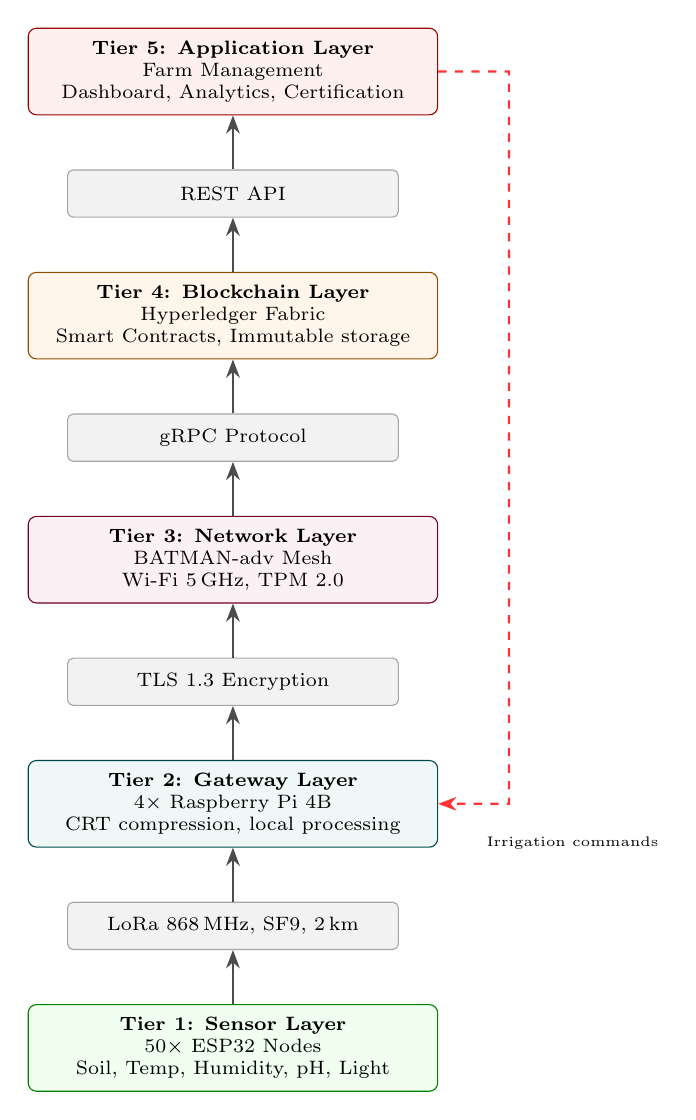
\begin{tikzpicture}[font=\scriptsize,
  tier/.style={draw, rounded corners=3pt, minimum width=5.2cm, minimum height=1.1cm,
               text centered, align=center, inner sep=4pt},
  proto/.style={draw=gray!70, fill=gray!10, rounded corners=2pt,
                minimum width=4.2cm, minimum height=0.6cm,
                text centered, align=center},
  arr/.style={-Stealth, thick, draw=black!70},
  redarr/.style={-Stealth, thick, dashed, draw=red!80}]

  % Tier boxes (bottom to top)
  \node[tier, fill=green!6,  draw=green!50!black]  (T1) at (0,0)
    {\textbf{Tier 1: Sensor Layer}\\50$\times$ ESP32 Nodes\\Soil, Temp, Humidity, pH, Light};

  \node[proto] (P12) at (0,1.55)
    {LoRa 868\,MHz, SF9, 2\,km};

  \node[tier, fill=teal!6,   draw=teal!60!black]   (T2) at (0,3.1)
    {\textbf{Tier 2: Gateway Layer}\\4$\times$ Raspberry Pi 4B\\CRT compression, local processing};

  \node[proto] (P23) at (0,4.65)
    {TLS 1.3 Encryption};

  \node[tier, fill=purple!6, draw=purple!60!black] (T3) at (0,6.2)
    {\textbf{Tier 3: Network Layer}\\BATMAN-adv Mesh\\Wi-Fi 5\,GHz, TPM 2.0};

  \node[proto] (P34) at (0,7.75)
    {gRPC Protocol};

  \node[tier, fill=orange!8, draw=orange!60!black] (T4) at (0,9.3)
    {\textbf{Tier 4: Blockchain Layer}\\Hyperledger Fabric\\Smart Contracts, Immutable storage};

  \node[proto] (P45) at (0,10.85)
    {REST API};

  \node[tier, fill=red!6,    draw=red!60!black]    (T5) at (0,12.4)
    {\textbf{Tier 5: Application Layer}\\Farm Management\\Dashboard, Analytics, Certification};

  % Upward arrows between tiers
  \draw[arr] (T1.north) to (P12.south);
  \draw[arr] (P12.north) to (T2.south);
  \draw[arr] (T2.north) to (P23.south);
  \draw[arr] (P23.north) to (T3.south);
  \draw[arr] (T3.north) to (P34.south);
  \draw[arr] (P34.north) to (T4.south);
  \draw[arr] (T4.north) to (P45.south);
  \draw[arr] (P45.north) to (T5.south);

  % Red dashed feedback arrow on right: Tier 5 -> Tier 2
  \draw[redarr] (T5.east) to ++(0.9,0) to ++(0,-9.3)
      to node[right=1pt, yshift=-0.5cm, font=\tiny]{Irrigation commands} (T2.east);
\end{tikzpicture}}%
\hfill
% Communication and control flow
\resizebox{!}{10cm}{%
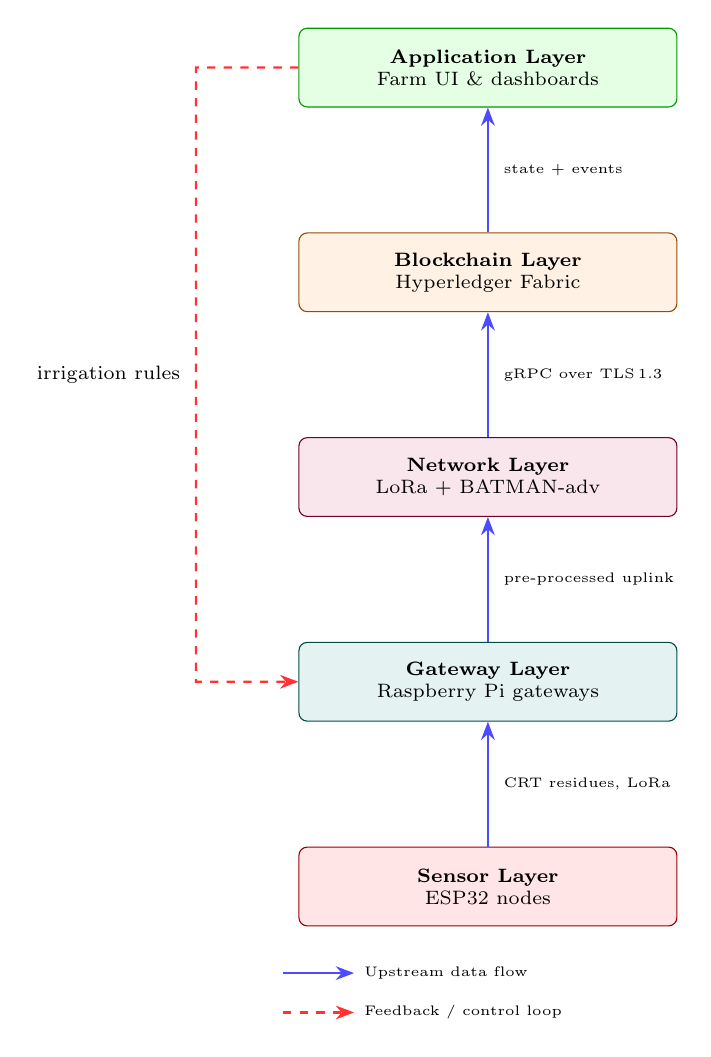
\begin{tikzpicture}[font=\scriptsize,
  layer/.style={draw, rounded corners=3pt, minimum width=4.8cm, minimum height=1.0cm,
                text centered, align=center, inner sep=4pt},
  uarr/.style={-Stealth, thick, draw=blue!70},
  darr/.style={-Stealth, thick, dashed, draw=red!80}]

  % Layer boxes bottom to top
  \node[layer, fill=red!10,    draw=red!60!black]    (S)  at (0,0)
    {\textbf{Sensor Layer}\\ESP32 nodes};
  \node[layer, fill=teal!10,   draw=teal!60!black]   (GW) at (0,2.6)
    {\textbf{Gateway Layer}\\Raspberry Pi gateways};
  \node[layer, fill=purple!10, draw=purple!60!black] (NW) at (0,5.2)
    {\textbf{Network Layer}\\LoRa + BATMAN-adv};
  \node[layer, fill=orange!10, draw=orange!60!black] (BC) at (0,7.8)
    {\textbf{Blockchain Layer}\\Hyperledger Fabric};
  \node[layer, fill=green!10,  draw=green!60!black]  (AP) at (0,10.4)
    {\textbf{Application Layer}\\Farm UI \& dashboards};

  % Upstream blue arrows
  \draw[uarr] (S.north)  to node[right=2pt, font=\tiny]{CRT residues, LoRa} (GW.south);
  \draw[uarr] (GW.north) to node[right=2pt, font=\tiny]{pre-processed uplink} (NW.south);
  \draw[uarr] (NW.north) to node[right=2pt, font=\tiny]{gRPC over TLS\,1.3} (BC.south);
  \draw[uarr] (BC.north) to node[right=2pt, font=\tiny]{state + events} (AP.south);

  % Red dashed feedback on left: App -> Gateway
  \draw[darr] (AP.west) to ++(-1.3,0) to node[left=2pt]{irrigation rules} ++(0,-7.8) to (GW.west);

  % Legend (drawn directly, avoids inline-tikz bounding-box issues)
  \draw[uarr] (-2.6,-1.1) to (-1.7,-1.1)
      node[right, font=\tiny]{Upstream data flow};
  \draw[darr] (-2.6,-1.6) to (-1.7,-1.6)
      node[right, font=\tiny]{Feedback / control loop};
\end{tikzpicture}}%
\caption{(a) System architecture tiers. (b) Vertical communication and control across the five-tier architecture.}
\label{fig:both}
\end{figure*}

\emph{Edge node} refers to the four Raspberry Pi 4B gateways performing local CRT reconstruction, Ed25519 verification, and irrigation decisions, not MEC in a cellular sense. Cloud round-trips cannot guarantee the 2\,s SLO given intermittent Sfax rural connectivity. Figure~\ref{fig:enhanced-farm-layout} shows the network topology.

\subsection{Farm Layout and Network Topology}
\label{subsec:farm_layout}

The 2-hectare farm (200\,m $\times$ 100\,m) was divided into four zones, each with 12 to 13 sensor nodes on a 20\,m grid.

\begin{figure*}[!htbp]
  \centering
  \resizebox{\linewidth}{!}{%
  \begin{tikzpicture}[font=\scriptsize,
    gw/.style={draw=red!80!black, fill=red!30, minimum size=0.5cm, inner sep=1pt, align=center},
    snode/.style={circle, draw=blue!70, fill=blue!40, minimum size=0.22cm, inner sep=0pt},
    mesh/.style={draw=red!70, line width=1.5pt},
    lora/.style={draw=blue!50, dashed, thin}]

    % Farm rectangle 20x10 (1 unit = 10 m)
    \draw[fill=green!8, draw=black] (0,0) rectangle (20,10);

    % Zone labels
    \node at (3,7.5)  {Zone 1};
    \node at (17,7.5) {Zone 2};
    \node at (3,2.5)  {Zone 3};
    \node at (17,2.5) {Zone 4};

    % Gateway positions
    \node[gw] (NGW) at (5,8.5)   {};
    \node[gw] (SGW) at (15,1.5)  {};
    \node[gw] (WGW) at (0.5,5)   {};
    \node[gw] (EGW) at (19.5,5)  {};

    % Gateway labels
    \node[above=2pt of NGW, align=center, font=\tiny] {N-GW\\RPi 4B};
    \node[below=2pt of SGW, align=center, font=\tiny] {S-GW\\RPi 4B};
    \node[above=2pt of WGW, align=center, font=\tiny] {W-GW\\RPi 4B};
    \node[above=2pt of EGW, align=center, font=\tiny] {E-GW\\RPi 4B};

    % BATMAN-adv mesh: connect all gateways
    \draw[mesh] (NGW) to (WGW);
    \draw[mesh] (NGW) to (EGW);
    \draw[mesh] (NGW) to (SGW);
    \draw[mesh] (WGW) to (SGW);
    \draw[mesh] (EGW) to (SGW);
    \draw[mesh] (WGW) to (EGW);

    % Sensor nodes (grid, ~50 nodes)
    \foreach \x/\y in {
      2/2, 2/4, 2/6, 2/8,
      4/2, 4/4, 4/6, 4/8,
      6/2, 6/4, 6/6, 6/8,
      8/2, 8/4, 8/6, 8/8,
      10/2,10/4,10/6,10/8,
      12/2,12/4,12/6,12/8,
      14/2,14/4,14/6,14/8,
      16/2,16/4,16/6,16/8,
      18/2,18/4,18/6,18/8,
      3/1, 7/1,11/1,15/1,19/1,
      3/9, 7/9,11/9,15/9,19/9,
      1/3, 1/5, 1/7,19/3}{
      \node[snode] at (\x,\y) {};
    }

    % Representative LoRa links (a few per zone)
    \draw[lora] (2,8) to (NGW);
    \draw[lora] (4,6) to (NGW);
    \draw[lora] (1,7) to (WGW);
    \draw[lora] (1,5) to (WGW);
    \draw[lora] (18,8) to (EGW);
    \draw[lora] (18,6) to (EGW);
    \draw[lora] (14,2) to (SGW);
    \draw[lora] (16,2) to (SGW);

    % X-axis scale (10 m per unit), placed inside rectangle at y=0
    \foreach \x/\lbl in {0/0, 4/40, 8/80, 12/120, 16/160, 20/200}{
      \draw (\x,0) to (\x,-0.15);
      \node[below, font=\tiny] at (\x,-0.15) {\lbl\,m};
    }
    \draw[->] (-0.2,-0.2) to (20.5,-0.2) node[right, font=\tiny]{x (m)};

    % Y-axis scale
    \foreach \y/\lbl in {0/0, 2/20, 4/40, 6/60, 8/80, 10/100}{
      \draw (0,\y) to (-0.15,\y);
      \node[left, font=\tiny] at (-0.15,\y) {\lbl\,m};
    }
    \draw[->] (-0.2,-0.2) to (-0.2,10.5) node[above, font=\tiny]{y (m)};

    % Legend below farm rectangle
    \node[draw=black!30, fill=white, rounded corners=2pt,
          inner sep=4pt, anchor=north] at (10,-0.75) {%
      \begin{tikzpicture}[font=\tiny,
          snode/.style={circle,draw=blue!70,fill=blue!40,minimum size=0.18cm,inner sep=0pt},
          gw/.style={draw=red!80!black,fill=red!30,minimum size=0.38cm,inner sep=0pt},
          mesh/.style={draw=red!70,line width=1.2pt},
          lora/.style={draw=blue!50,dashed,thin}]
        \node[snode] at (0,0) {};
        \node[right=4pt, font=\tiny] at (0.12,0) {ESP32 Sensor};
        \node[gw] at (2.7,0) {};
        \node[right=4pt, font=\tiny] at (2.82,0) {RPi Gateway};
        \draw[mesh] (5.4,0) to (6.0,0);
        \node[right=4pt, font=\tiny] at (6.0,0) {BATMAN-adv};
        \draw[lora] (8.5,0) to (9.1,0);
        \node[right=4pt, font=\tiny] at (9.1,0) {LoRa link};
        \draw[|-|, thick] (11.3,0) to (13.3,0)
            node[midway, below=2pt, font=\tiny]{20\,m};
      \end{tikzpicture}%
    };
  \end{tikzpicture}}%
  \caption{Hybrid LoRa-mesh network architecture with 50 ESP32 sensor nodes, 4 Raspberry Pi gateways, and BATMAN-adv backbone for reliable data aggregation.}
  \label{fig:enhanced-farm-layout}
\end{figure*}

\subsection{Distributed Parallel Computing Architecture}
\label{subsec:parallel_arch}

The ESP32’s dual Xtensa LX6 cores \cite{espressif2020esp32} run sensor sampling (Core~0, 8.0\,ms) and CRT decomposition + LoRa preparation (Core~1, 0.9\,ms) in parallel; the critical path is 8.0\,ms, confirming negligible CRT overhead.

The SX1302 multi-channel concentrator demodulates one packet per channel simultaneously, so gateway packet throughput on a single channel is $\lambda = 1/T_{\text{airtime}}$, giving:
\begin{equation}
\lambda_{\text{raw}} = \frac{1}{247\,\text{ms}} \approx 4.05\ \text{pkt/s}, \qquad
\lambda_{\text{CRT}} = \frac{1}{124\,\text{ms}} \approx 8.06\ \text{pkt/s}.
\label{eq:packet_rates}
\end{equation}
The per-channel packet-rate improvement is therefore
\begin{equation}
\frac{\lambda_{\text{CRT}}}{\lambda_{\text{raw}}} = \frac{T_{\text{raw}}}{T_{\text{CRT}}} = \frac{247}{124} \approx 1.99\times,
\label{eq:throughput_improvement}
\end{equation}
consistent with the packet-capacity ratio derived from first principles in Section~\ref{subsec:crt_transmission} ($P_{\max}^{\text{CRT}}=1{,}451$ vs.\ $P_{\max}^{\text{raw}}=728 \approx 2\times$). Per-node airtime rises from 247 to 372\,ms (three sequential packets); the gain is gateway packet capacity, not per-node energy. The four RPi 4B gateways form a homogeneous cluster with BATMAN-adv mesh (sub-second failover) and per-gateway Fabric peer + CouchDB, sustaining blockchain consensus and real-time actuation locally; performance is in Section~\ref{subsec:blockchain_performance}.

\subsection{Hardware Design and Implementation}
\label{subsec:hardware}

Each sensor node used an ESP32-WROOM-32 microcontroller \cite{espressif2020esp32} with sensors listed in Table~\ref{tab:sensor-specs}.

\begin{table}[!t]
\centering
\caption{Sensor node specifications and components}
\label{tab:sensor-specs}
\begin{tabularx}{\linewidth}{l X X}
\toprule
\textbf{Component} & \textbf{Specification} & \textbf{Purpose} \\
\midrule
Microcontroller & ESP32-WROOM-32 & Main processing and control \\
Soil Moisture & TDR-315N & Volumetric water content \\
Temperature & DHT22 & Ambient temperature \\
Humidity & DHT22 & Relative humidity \\
pH Sensor & Analog with amplifier & Soil acidity \\
Light Sensor & BH1750 & Photosynthetic radiation \\
Communication & RFM95W LoRa & Long-range data transmission \cite{adafruit2016rfm95w} \\
Power & 18650 Li-ion, 2,600~mAh / 3.7~V / 9.62~Wh + 2\,W, 6\,V monocrystalline silicon PV panel & Energy supply and storage \\
\bottomrule
\end{tabularx}
\end{table}

\begin{sidewaysfigure}[!htbp]
  \centering
  \resizebox{0.94\textheight}{!}{%
  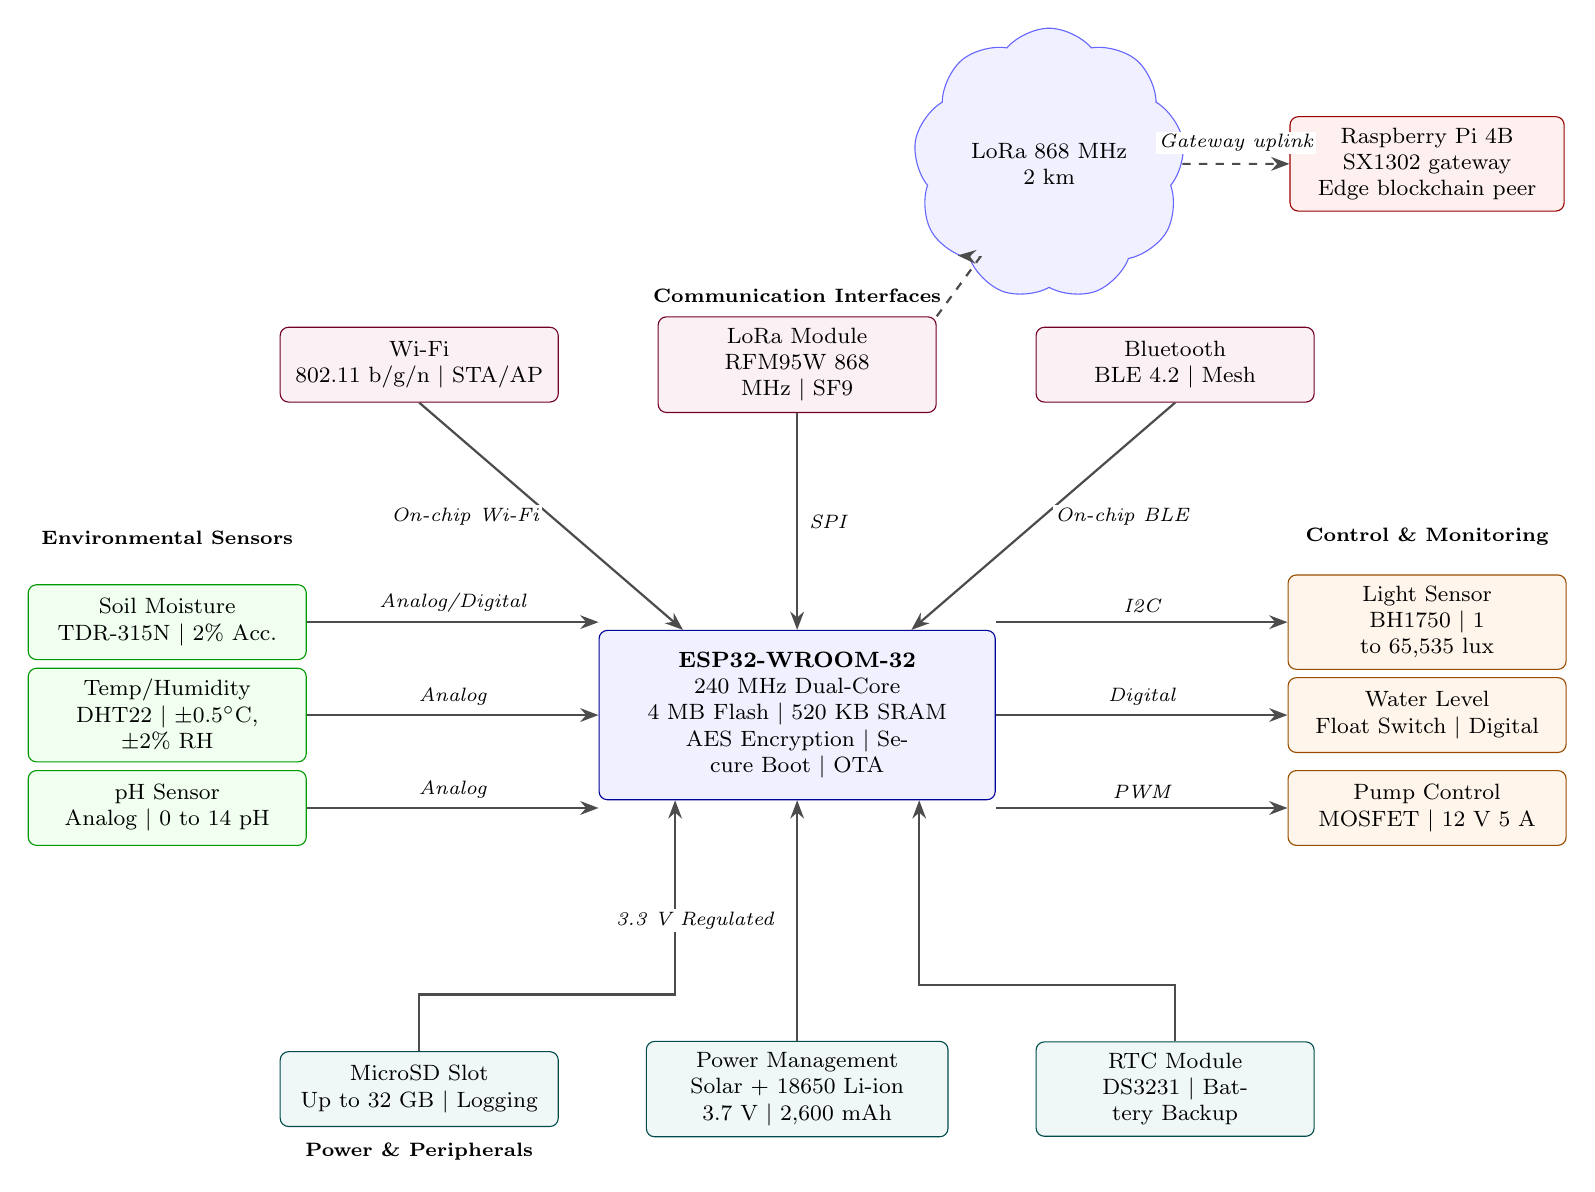
\begin{tikzpicture}[font=\footnotesize,
    cbox/.style={draw, rounded corners=3pt, minimum height=0.95cm,
                 align=center, inner sep=4pt, text width=3.25cm},
    arr/.style={-Stealth, thick, draw=black!70},
    labl/.style={font=\scriptsize\itshape, midway, fill=white, inner sep=1pt}]

    % Central ESP32 block
    \node[cbox, fill=blue!6, draw=blue!60!black, minimum width=5.0cm, minimum height=2.15cm,
          text width=4.75cm] (esp) at (0,0)
      {\textbf{ESP32-WROOM-32}\\240 MHz Dual-Core\\4 MB Flash $|$ 520 KB SRAM\\AES Encryption $|$ Secure Boot $|$ OTA};

    % === LEFT: Environmental Sensors ===
    \node[font=\scriptsize\bfseries, fill=white, inner sep=1pt, anchor=south] at (-8.0, 2.12) {Environmental Sensors};

    \node[cbox, fill=green!6, draw=green!60!black] (SM) at (-8.0, 1.18)
      {Soil Moisture\\TDR-315N $|$ 2\% Acc.};
    \node[cbox, fill=green!6, draw=green!60!black] (TH) at (-8.0, 0)
      {Temp/Humidity\\DHT22 $|$ $\pm$0.5$^\circ$C, $\pm$2\% RH};
    \node[cbox, fill=green!6, draw=green!60!black] (pH) at (-8.0,-1.18)
      {pH Sensor\\Analog $|$ 0 to 14 pH};

    \draw[arr] (SM.east) to node[pos=0.62, above=2pt, labl]{Analog/Digital} (esp.west |- SM.east);
    \draw[arr] (TH.east) to node[pos=0.62, above=2pt, labl]{Analog} (esp.west |- TH.east);
    \draw[arr] (pH.east) to node[pos=0.62, above=2pt, labl]{Analog} (esp.west |- pH.east);

    % === RIGHT: Control & Monitoring ===
    \node[font=\scriptsize\bfseries, fill=white, inner sep=1pt, anchor=south] at (8.0, 2.12) {Control \& Monitoring};

    \node[cbox, fill=orange!8, draw=orange!60!black] (LS) at (8.0, 1.18)
      {Light Sensor\\BH1750 $|$ 1 to 65,535 lux};
    \node[cbox, fill=orange!8, draw=orange!60!black] (WL) at (8.0, 0)
      {Water Level\\Float Switch $|$ Digital};
    \node[cbox, fill=orange!8, draw=orange!60!black] (PC) at (8.0,-1.18)
      {Pump Control\\MOSFET $|$ 12 V 5 A};

    \draw[arr] (esp.east |- LS.west) to node[pos=0.38, above=2pt, labl]{I2C}     (LS.west);
    \draw[arr] (esp.east |- WL.west) to node[pos=0.38, above=2pt, labl]{Digital}  (WL.west);
    \draw[arr] (esp.east |- PC.west) to node[pos=0.38, above=2pt, labl]{PWM}      (PC.west);

    % === TOP: Communication Interfaces ===
    \node[font=\scriptsize\bfseries, fill=white, inner sep=1pt] at (0, 5.32) {Communication Interfaces};

    \node[cbox, fill=purple!6, draw=purple!60!black] (WIFI) at (-4.8, 4.45)
      {Wi-Fi\\802.11 b/g/n $|$ STA/AP};
    \node[cbox, fill=purple!6, draw=purple!60!black] (LORA) at (0, 4.45)
      {LoRa Module\\RFM95W 868 MHz $|$ SF9};
    \node[cbox, fill=purple!6, draw=purple!60!black] (BLE)  at (4.8, 4.45)
      {Bluetooth\\BLE 4.2 $|$ Mesh};

    \draw[arr] (WIFI.south) to node[pos=0.48, left=3pt, labl]{On-chip Wi-Fi} ([xshift=-1.45cm]esp.north);
    \draw[arr] (LORA.south) to node[pos=0.42, right=3pt, labl]{SPI}    (esp.north);
    \draw[arr] (BLE.south)  to node[pos=0.48, right=3pt, labl]{On-chip BLE} ([xshift=1.45cm]esp.north);

    % LoRa wireless link to gateway
    \node[cloud, cloud puffs=9, cloud puff arc=100,
          draw=blue!60, fill=blue!6, minimum width=2.45cm, minimum height=1.10cm,
          align=center] (cloud) at (3.2, 7.0)
      {LoRa 868 MHz\\2 km};
    \node[cbox, fill=red!6, draw=red!60!black, minimum width=3.45cm, text width=3.2cm]
      (rpi) at (8.0, 7.0)
      {Raspberry Pi 4B\\SX1302 gateway\\Edge blockchain peer};
    \draw[arr, dashed] (LORA.north east) to ++(0.55,0.75) to (cloud.south west);
    \draw[arr, dashed] (cloud.east) to node[pos=0.54, above=3pt, labl]{Gateway uplink} (rpi.west);

    % === BOTTOM: Power & Peripherals ===
    \node[font=\scriptsize\bfseries, fill=white, inner sep=1pt] at (-4.8,-5.55) {Power \& Peripherals};

    \node[cbox, fill=teal!6, draw=teal!60!black] (SD) at (-4.8,-4.75)
      {MicroSD Slot\\Up to 32 GB $|$ Logging};
    \node[cbox, fill=teal!6, draw=teal!60!black, text width=3.55cm] (PM) at (0,-4.75)
      {Power Management\\Solar + 18650 Li-ion\\3.7 V $|$ 2,600 mAh};
    \node[cbox, fill=teal!6, draw=teal!60!black] (RTC) at (4.8,-4.75)
      {RTC Module\\DS3231 $|$ Battery Backup};

    \draw[arr] (SD.north)  to ++(0,0.72) -| ([xshift=-1.55cm]esp.south);
    \draw[arr] (PM.north)  to node[pos=0.43, left=7pt, labl]{3.3 V Regulated} (esp.south);
    \draw[arr] (RTC.north) to ++(0,0.72) -| ([xshift=1.55cm]esp.south);

  \end{tikzpicture}}%
  \caption{ESP32 sensor node with sensor inputs, communication modules, and LoRa link to Raspberry Pi gateway for agricultural IoT.}
  \label{fig:enhanced-sensor-node}
\end{sidewaysfigure}

\subsubsection{Scalability and Node Count Validation}
\label{subsubsec:scalability_analysis_related}

The deployment (50 nodes, 2\,ha, 146,400 transactions) gives theoretical capacity $N_{\max} = C W / (k T_{\text{packet}})$ (Eq.~\ref{eq:scalability}); Table~\ref{tab:scalability-comparison} lists results for raw and CRT.
\begin{equation}
N_{\max} = \frac{C \cdot W}{k \cdot T_{\text{packet}}},
\label{eq:scalability}
\end{equation}

\begin{table}[htbp]
\centering
\caption{Theoretical node capacity: raw vs.\ CRT transmission ($W = 60$\,s channel time window used for slot counting; actual polling interval is 30\,min)}
\label{tab:scalability-comparison}
\begin{tabular}{lcc}
\toprule
\textbf{Parameter}                & \textbf{Raw} & \textbf{CRT} \\
\midrule
Per-packet airtime (ms)           & 247           & 124           \\
Packets per reading               & 1             & 3             \\
Maximum nodes $N_{\max}$           & 728           & 484           \\
Relative node capacity             & 1.0           & 0.66          \\
\bottomrule
\end{tabular}
\end{table}

CRT halves per-packet airtime but requires 3 packets, yielding $N_{\max}=484$ vs.\ raw’s 728. The 50-node deployment uses 10\% of capacity.

\subsubsection{Gateway Architecture}
Each RPi 4B gateway (4\,GB RAM \cite{rpi2023specs}) hosts an SX1302 LoRa concentrator \cite{waveshare2024sx1302}, TPM\,2.0 \cite{microsoft2023tpm}, dual-band Wi-Fi (BATMAN-adv), 128\,GB microSD, and GPS. Pipeline: receive CRT residues, apply Garner reconstruction, verify Ed25519 signatures and timestamps, trigger threshold-based local irrigation, and anchor the Fabric hash (Figure~\ref{fig:gateway-architecture}). \textbf{Deployment requirement:} SX1302-class multi-channel concentrator is mandatory; single-channel transceivers serialize reception and negate CRT’s network-density benefit.

\begin{sidewaysfigure}[!htbp]
  \centering
  \resizebox{0.95\textheight}{!}{%
  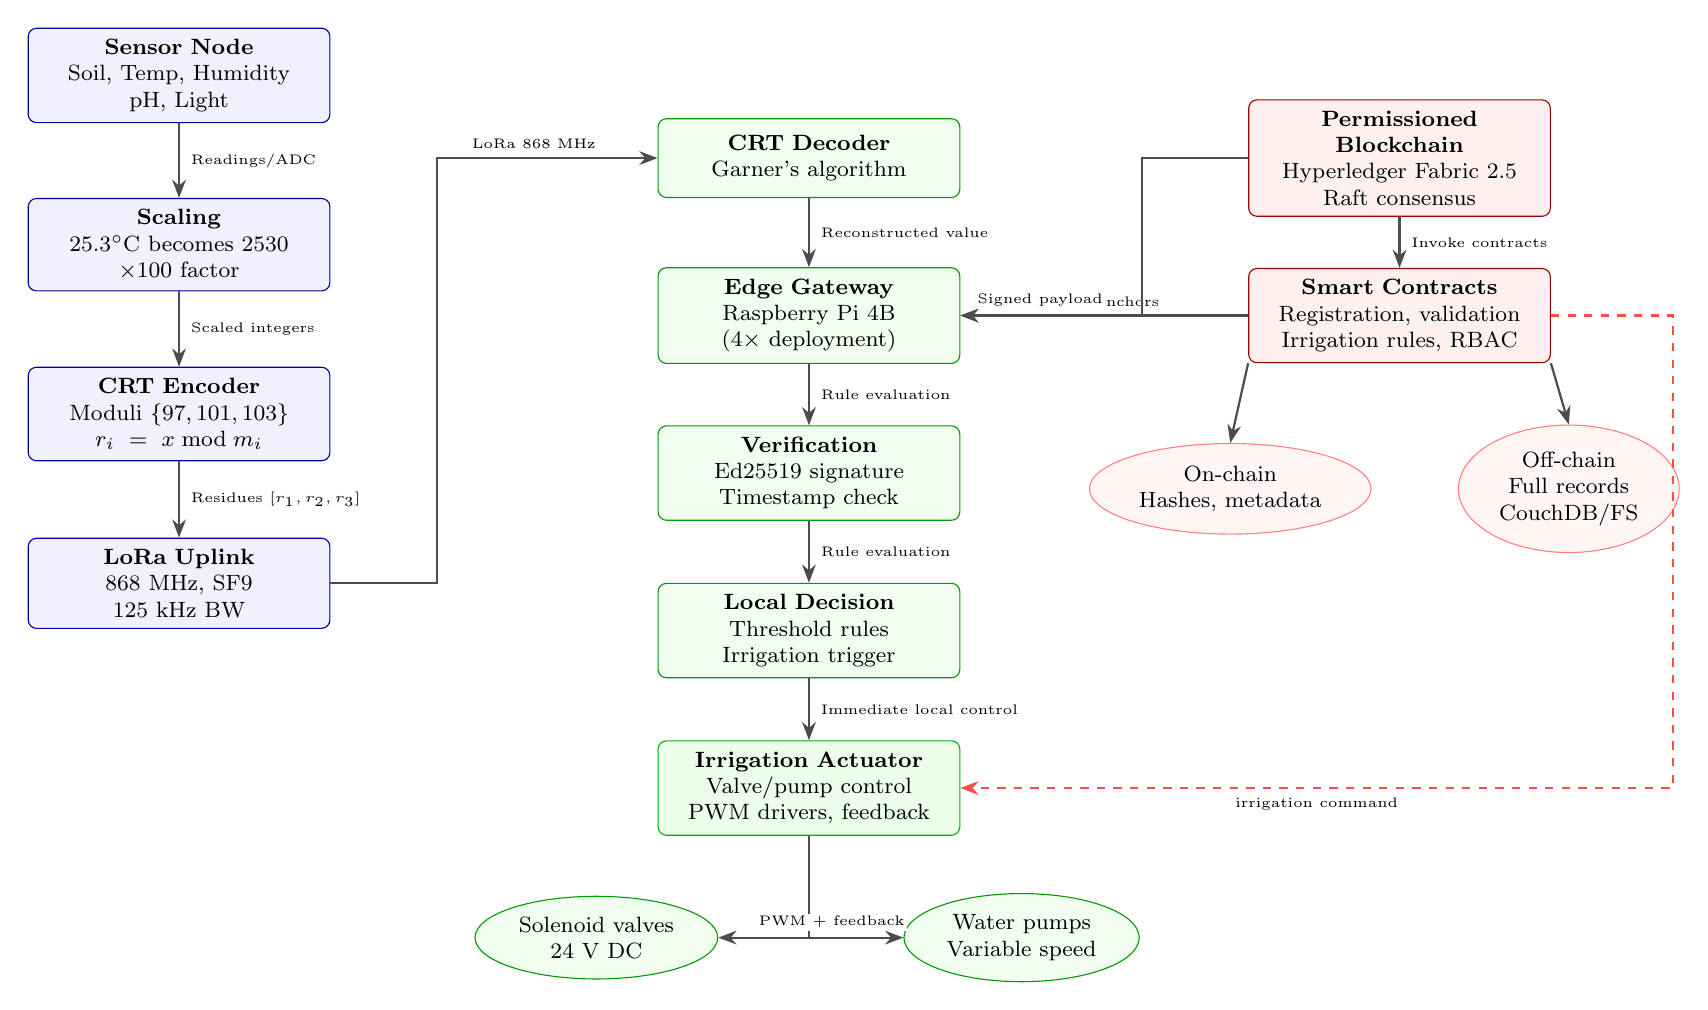
\begin{tikzpicture}[font=\footnotesize,
    bbox/.style={draw, rounded corners=3pt, minimum width=3.8cm, minimum height=1.0cm,
                 align=center, inner sep=4pt, text width=3.55cm},
    store/.style={draw=red!50, fill=red!4, ellipse, minimum width=2.7cm,
                  minimum height=1.15cm, align=center, inner sep=3pt},
    actuator/.style={draw=green!60!black, fill=green!6, ellipse, minimum width=2.8cm,
                     minimum height=1.05cm, align=center, inner sep=3pt},
    arr/.style={-Stealth, thick, draw=black!70},
    rarr/.style={-Stealth, thick, draw=red!70, dashed},
    lab/.style={font=\tiny, fill=white, inner sep=1pt}]

    % ============ LEFT COLUMN: Sensor side ============
    \node[bbox, fill=blue!6, draw=blue!60!black] (SN) at (-8.0, 9.6)
      {\textbf{Sensor Node}\\Soil, Temp, Humidity\\pH, Light};
    \node[bbox, fill=blue!6, draw=blue!60!black] (SC) at (-8.0, 7.45)
      {\textbf{Scaling}\\25.3$^\circ$C becomes 2530\\$\times$100 factor};
    \node[bbox, fill=blue!6, draw=blue!60!black] (CE) at (-8.0, 5.3)
      {\textbf{CRT Encoder}\\Moduli $\{97,101,103\}$\\$r_i = x \bmod m_i$};
    \node[bbox, fill=blue!6, draw=blue!60!black] (LU) at (-8.0, 3.15)
      {\textbf{LoRa Uplink}\\868 MHz, SF9\\125 kHz BW};

    \draw[arr] (SN.south) to node[right=3pt, lab]{Readings/ADC} (SC.north);
    \draw[arr] (SC.south) to node[right=3pt, lab]{Scaled integers} (CE.north);
    \draw[arr] (CE.south) to node[right=3pt, lab]{Residues $[r_1,r_2,r_3]$} (LU.north);

    % ============ CENTER COLUMN: Gateway ============
    \node[bbox, fill=green!6, draw=green!60!black] (CD) at (0, 8.55)
      {\textbf{CRT Decoder}\\Garner's algorithm};
    \node[bbox, fill=green!6, draw=green!60!black] (GW) at (0, 6.55)
      {\textbf{Edge Gateway}\\Raspberry Pi 4B\\(4$\times$ deployment)};
    \node[bbox, fill=green!6, draw=green!60!black] (VF) at (0, 4.55)
      {\textbf{Verification}\\Ed25519 signature\\Timestamp check};
    \node[bbox, fill=green!6, draw=green!60!black] (LD) at (0, 2.55)
      {\textbf{Local Decision}\\Threshold rules\\Irrigation trigger};
    \node[bbox, fill=green!8, draw=green!70!black] (IA) at (0, 0.55)
      {\textbf{Irrigation Actuator}\\Valve/pump control\\PWM drivers, feedback};

    % LoRa link, kept clear of the center boxes
    \draw[arr] (LU.east) to ++(1.35,0) |- node[pos=0.72, above=2pt, lab]{LoRa 868 MHz} (CD.west);
    \draw[arr] (CD.south) to node[right=3pt, lab]{Reconstructed value} (GW.north);
    \draw[arr] (GW.south) to node[right=3pt, lab]{Rule evaluation} (VF.north);
    \draw[arr] (VF.south) to node[right=3pt, lab]{Rule evaluation} (LD.north);
    \draw[arr] (LD.south) to node[right=3pt, lab]{Immediate local control} (IA.north);

    % Actuator outputs
    \node[actuator] (SV) at (-2.7, -1.35) {Solenoid valves\\24 V DC};
    \node[actuator] (WP) at (2.7, -1.35)  {Water pumps\\Variable speed};

    \draw[arr] (IA.south) |- (SV.east);
    \draw[arr] (IA.south) |- node[pos=0.62, above=2pt, lab]{PWM + feedback} (WP.west);

    % ============ RIGHT COLUMN: Blockchain ============
    \node[bbox, fill=red!6, draw=red!60!black] (BC) at (7.5, 8.55)
      {\textbf{Permissioned Blockchain}\\Hyperledger Fabric 2.5\\Raft consensus};
    \node[bbox, fill=red!6, draw=red!60!black] (SC2) at (7.5, 6.55)
      {\textbf{Smart Contracts}\\Registration, validation\\Irrigation rules, RBAC};

    \node[store] (ONc) at (5.35, 4.35)  {On-chain\\Hashes, metadata};
    \node[store] (OFc) at (9.65, 4.35)  {Off-chain\\Full records\\CouchDB/FS};

    \draw[arr] (BC.south)  to node[right=3pt, lab]{Invoke contracts} (SC2.north);
    \draw[arr] (SC2.west)  to node[above=2pt, lab]{Hash anchors} (GW.east);
    \draw[arr] (SC2.south west) to (ONc.north);
    \draw[arr] (SC2.south east) to (OFc.north);

    % Signed payload from blockchain back to gateway, routed above the gateway column
    \draw[arr] (BC.west) to ++(-1.35,0) |- node[pos=0.78, above=2pt, lab]{Signed payload} (GW.east);

    % Blockchain irrigation command event routed outside all boxes
    \draw[rarr] (SC2.east) to ++(1.55,0) to ++(0,-6.0) to node[below=2pt, lab]{irrigation command} (IA.east);

  \end{tikzpicture}}%
  \caption{Raspberry Pi 4B gateway architecture showing data processing pipeline and security modules}
  \label{fig:gateway-architecture}
\end{sidewaysfigure}

\subsection{Node Communication Protocol}
\label{subsec:communication_protocol}

\subsubsection{LoRa Communication Framework and MAC-Layer Residue Channel Coordination}
\label{subsubsec:lora_mac}

Sensor nodes communicated with gateways in the EU868 ISM band \cite{ttn2024eu868,loraalliance2021regional} using a hybrid scheduling policy:
\begin{itemize}
  \item \textbf{Periodic polling:} each gateway solicits its zone's nodes every 30 minutes.
  \item \textbf{Event-driven uplink:} nodes transmit immediately on soil-moisture or temperature threshold breach, superimposed on the polling schedule.
  \item \textbf{Acknowledged delivery:} every uplink receives a gateway ACK within one guard interval; unacknowledged packets are retried once.
\end{itemize}

\paragraph{Static residue-channel assignment.}
The three CRT residue packets of each reading are assigned to fixed sub-channels: residue~$r_1$ on 868.1\,MHz, $r_2$ on 868.3\,MHz, $r_3$ on 868.5\,MHz (125\,kHz BW, SF9). A node sends the three packets \emph{sequentially} with the same spreading factor; the gateway's SX1302 concentrator receives packets from \emph{different} nodes on the three channels \emph{concurrently}. SPI channel switching between residues adds $\approx$1\,ms overhead per hop, negligible against the 124\,ms packet airtime.

\paragraph{Per-zone sequential polling schedule.}
The 50-node deployment is partitioned into four geographic zones ($Z_1$--$Z_4$, each covering one gateway quadrant, 12--13 nodes per zone). Each gateway independently executes the polling round for its zone inside a dedicated $T_{\text{zone}} = T_w/4 = 450$\,s slot within the 30-minute reporting window ($T_w = 1800$\,s):
\begin{enumerate}
  \item The gateway broadcasts a \textsc{Poll}(\textit{node\_id}) frame on 868.1\,MHz.
  \item The addressed node replies with its three residue packets sequentially across 868.1/868.3/868.5\,MHz; total node airtime is $3 \times 124\,\text{ms} = 372$\,ms.
  \item After a fixed guard interval $T_g = 50$\,ms (ACK turnaround + processing), the gateway issues the next \textsc{Poll}.
  \item Per-node slot: $T_{\text{node}} = 372 + 50 = 422$\,ms.
\end{enumerate}
A zone with 13 nodes completes its round in $13 \times 422\,\text{ms} \approx 5.5$\,s, using only $5.5/450 \approx 1.2\%$ of its allocated slot. The remaining slot time absorbs event-driven uplinks, retransmissions, and ACK overhead without risking inter-zone interference. Zone polling rounds are \emph{not} globally synchronised; each gateway begins its round offset by a 10\,s per-gateway jitter seeded from the gateway serial number to decorrelate simultaneous starts.

\paragraph{Collision probability analysis.}
Because each zone's gateway polls its nodes one at a time, intra-zone collisions are structurally impossible. Cross-zone collisions can occur when two gateways poll their respective current node at the same instant \emph{and} both nodes are transmitting the same residue index (hence the same sub-channel).

We bound the collision probability using the Poisson offered-load model for LoRaWAN channel capacity \cite{bor2016lorawan,adelantado2017understanding}. Over a single reporting window, each of the $N = 50$ nodes transmits one packet on each of the three channels. The offered load per channel is:
\begin{equation}
G = \frac{N \cdot T_{\text{air}}}{T_w} = \frac{50 \times 0.124\,\text{s}}{1800\,\text{s}} = 3.44 \times 10^{-3}\ \text{Erlang}.
\label{eq:channel_load}
\end{equation}
Under a pure-ALOHA worst case (no scheduling), the per-packet collision probability is:
\begin{equation}
P_{\text{coll}}^{\text{ALOHA}} = 1 - e^{-2G} \approx 2G = 6.9 \times 10^{-3}\ (0.69\%).
\label{eq:p_coll_aloha}
\end{equation}
Per-zone sequential polling serialises intra-zone traffic, reducing collision risk below this bound. The residual cross-zone risk arises from unsynchronised polling across the four gateways. For a given packet on channel~$k$ from zone~$A$, the probability of a same-channel collision with \emph{any} of the $n_z = 13$ transmissions that a peer zone~$B$ schedules on channel~$k$ across the full $T_w = 1800$\,s window is:
\begin{equation}
P_{\text{cross},B} = 1 - \!\left(1 - \frac{2\,T_{\text{air}}}{T_w}\right)^{\!n_z}
  \approx \frac{n_z \cdot 2\,T_{\text{air}}}{T_w}
  = \frac{13 \times 2 \times 0.124}{1800} \approx 1.79 \times 10^{-3},
\label{eq:p_cross_one}
\end{equation}
where the approximation holds because $2T_{\text{air}}/T_w = 1.38 \times 10^{-4} \ll 1$. Let $J = 4$ denote the total number of deployment zones (one per gateway quadrant: $Z_1$--$Z_4$); a packet in zone $A$ faces $J - 1 = 3$ peer zones that could generate a same-channel collision. Summing $P_{\text{cross},B}$ over the three peer zones:
\begin{equation}
P_{\text{cross}} = (J-1)\cdot P_{\text{cross},B} = 3 \times 1.79 \times 10^{-3} \approx 5.4 \times 10^{-3}\ (0.54\%).
\label{eq:p_cross_total}
\end{equation}
Adding event-driven traffic (observed peak: 10 concurrent uplinks during the Day-23 morning spike), the composite collision estimate remains $< 1\%$, consistent with the measured 4.1\% end-to-end packet loss (dominated by RF fading and low-battery conditions, not MAC collisions).

\paragraph{Regulatory duty-cycle compliance (ETSI EU868).}
The EU868 sub-band used for uplinks (868.0 to 868.6\,MHz) is limited to a 1\% per-device duty cycle under ETSI EN\,300\,220 \cite{ttn2024eu868,loraalliance2021regional}. Node-side compliance is comfortable at every density analysed in this paper: one reading per 30-minute window occupies $3 \times 124 = 372$\,ms, a duty cycle of $0.372/1800 = 0.021\%$, and even a worst case in which all three residue packets are retried once reaches only 0.041\% (the per-node figure is independent of network size, so it holds unchanged at $N_{\max} = 484$). The gateway downlink is the tighter budget because the polling protocol transmits one \textsc{Poll} frame plus three ACKs per node per window ($\approx 4 \times 124 = 496$\,ms at SF9). At the deployed scale (13 nodes in the busiest zone) this is $13 \times 0.496/1800 = 0.36\%$, compliant within the 1\% sub-band. At the theoretical capacity of 121 nodes per zone, however, downlink occupancy rises to $121 \times 0.496/1800 \approx 3.3\%$, exceeding the 1\% limit; dense deployments must therefore either (i) move gateway downlink traffic to the 869.4 to 869.65\,MHz sub-band, which permits a 10\% duty cycle at up to $+27$\,dBm ERP (the convention adopted by LoRaWAN for RX2 downlinks \cite{ttn2024eu868}), optionally combined with (ii) aggregating the three per-residue ACKs into a single per-reading ACK, which halves downlink load ($\approx$1.7\%, still above the 1\% sub-band limit on its own but comfortably within the 10\% sub-band). Neither option alters the capacity analysis above, which is computed from uplink airtime only.

\paragraph{Scalability ceiling and path to TDMA.}
The analysis above holds while channel load $G \ll 1$. At 50 nodes the system operates at $G = 0.34\%$ of channel capacity; even at the theoretical maximum of $N_{\max} = 484$ CRT nodes (Section~\ref{subsec:crt_transmission}), $G = 484 \times 0.124/1800 = 3.3\%$, giving $P_{\text{coll}}^{\text{ALOHA}} = 1 - e^{-2G} = 6.45\% < 6.6\%$. The per-zone sequential scheduler itself is not the binding constraint: a zone with $n_z$ nodes completes its polling round in $n_z \times T_{\text{node}}$; at $N_{\max} = 484$ nodes ($\approx 121$ per zone) this is $121 \times 422\,\text{ms} \approx 51\,\text{s}$, well within the 450\,s zone slot. The scheduler can accommodate up to $\lfloor 450\,\text{s} / 0.422\,\text{s} \rfloor \approx 1066$ nodes per zone (4264 total) before timing headroom is exhausted. The channel-capacity ceiling $N_{\max}$ (not the scheduling round) is therefore always the tighter constraint. Nevertheless, above $N_{\max}$ a time-division multiple-access (TDMA) frame with globally synchronised slot assignments, or a carrier-sense multiple-access (CSMA) scheme with back-off, would be required to maintain the $< 2\%$ collision target as channel load rises. This is identified as the primary MAC-layer extension for future work, alongside investigation of frequency-hopping spread spectrum (FHSS) to further decorrelate residue channels under dense deployments \cite{adelantado2017understanding,bor2016lorawan}.

\begin{table}[htbp]
\centering
\caption{LoRa communication parameters for node-gateway communication}
\label{tab:lora-params}
\begin{tabular}{lcc}
\toprule
\textbf{Parameter} & \textbf{Value} & \textbf{Description} \\
\midrule
Frequency          & 868.1 MHz & EU ISM band \\
Spreading Factor   & SF9       & Balance range and airtime \\
Bandwidth          & 125 kHz   & Standard LoRa bandwidth \\
Coding Rate        & 4/5       & Error correction rate \\
CRC                & on        & Enabled for data integrity \\
Data Rate          & 1.76 kbps & Effective data rate \\
Airtime (34B)$^\P$ & 247 ms    & Raw reference frame (sensor payload, no signature) \\
Airtime (8B)       & 124 ms    & CRT packet \\
\bottomrule
\end{tabular}
{\footnotesize $^\P$ The 34-byte raw reference frame comprises Node ID (2\,B),
timestamp (4\,B), five 4-byte sensor values (20\,B), battery level (1\,B),
and 7\,B of radio-layer MAC framing (frame counter, frame type, and reserved fields)
that is transparent to the application layer and therefore not shown in Table~\ref{tab:data-frame};
the 32-byte Ed25519 signature is excluded to isolate sensor-transmission overhead.
The complete 59-byte signed frame gives 349\,ms at SF9. The 49.8\% airtime
reduction quoted throughout (from 247 to 124\,ms) compares this raw reference
against the 8-byte CRT residue packet.}
\end{table}

\begin{table}[htbp]
\centering
\caption{Data frame structure for sensor node communication}
\label{tab:data-frame}
\begin{tabular}{p{2.2cm} c c p{4.5cm}}
\toprule
\textbf{Field} & \textbf{Size} & \textbf{CRT} & \textbf{Description} \\
\midrule
Node ID        & 2  & 2  & Unique identifier \\
Timestamp      & 4  & 4  & Unix timestamp \\
Soil Moisture  & 4  & 1  & VWC value \\
Temperature    & 4  & 1  & Celsius $\times 100$ \\
Humidity       & 4  & 1  & RH $\times 100$ \\
pH Value       & 4  & 1  & pH $\times 100$ \\
Light Intensity& 4  & 1  & Lux \\
Battery Level  & 1  & 1  & 0 to 100\% \\
Packet overhead& 0  & 3  & Channel ID, seq., type flag \\
Signature      & 32 & 32 & Ed25519 signature \\
\midrule
\textbf{Total} & \textbf{59} & \textbf{47} & \textbf{20\% reduction} \\
\bottomrule
\end{tabular}
\end{table}

\subsection{CRT-Blockchain Integration Architecture}
\label{subsec:crt_blockchain_integration}

Figure~\ref{fig:crt_blockchain_flow_unified} illustrates the complete data flow: CRT encoding, digital signing, LoRa transmission, gateway verification and reconstruction, smart-contract validation, on-chain SHA-256 hash anchoring, and off-chain record storage. Together, these stages provide a tamper-evident audit trail and multi-party access without shared credentials.

The pipeline deliberately separates fast edge processing from slower but verifiable ledger operations. The gateway first reconstructs and validates each sensor reading locally so irrigation decisions can be issued without waiting for cloud services. The blockchain layer then records a compact hash anchor and access-control decision, while the full time-series record remains in off-chain storage for dashboard queries and certification audits. This separation keeps the real-time control path lightweight while preserving traceability for later verification.


\begin{sidewaysfigure}[p]
\centering
\resizebox{0.98\textheight}{!}{%
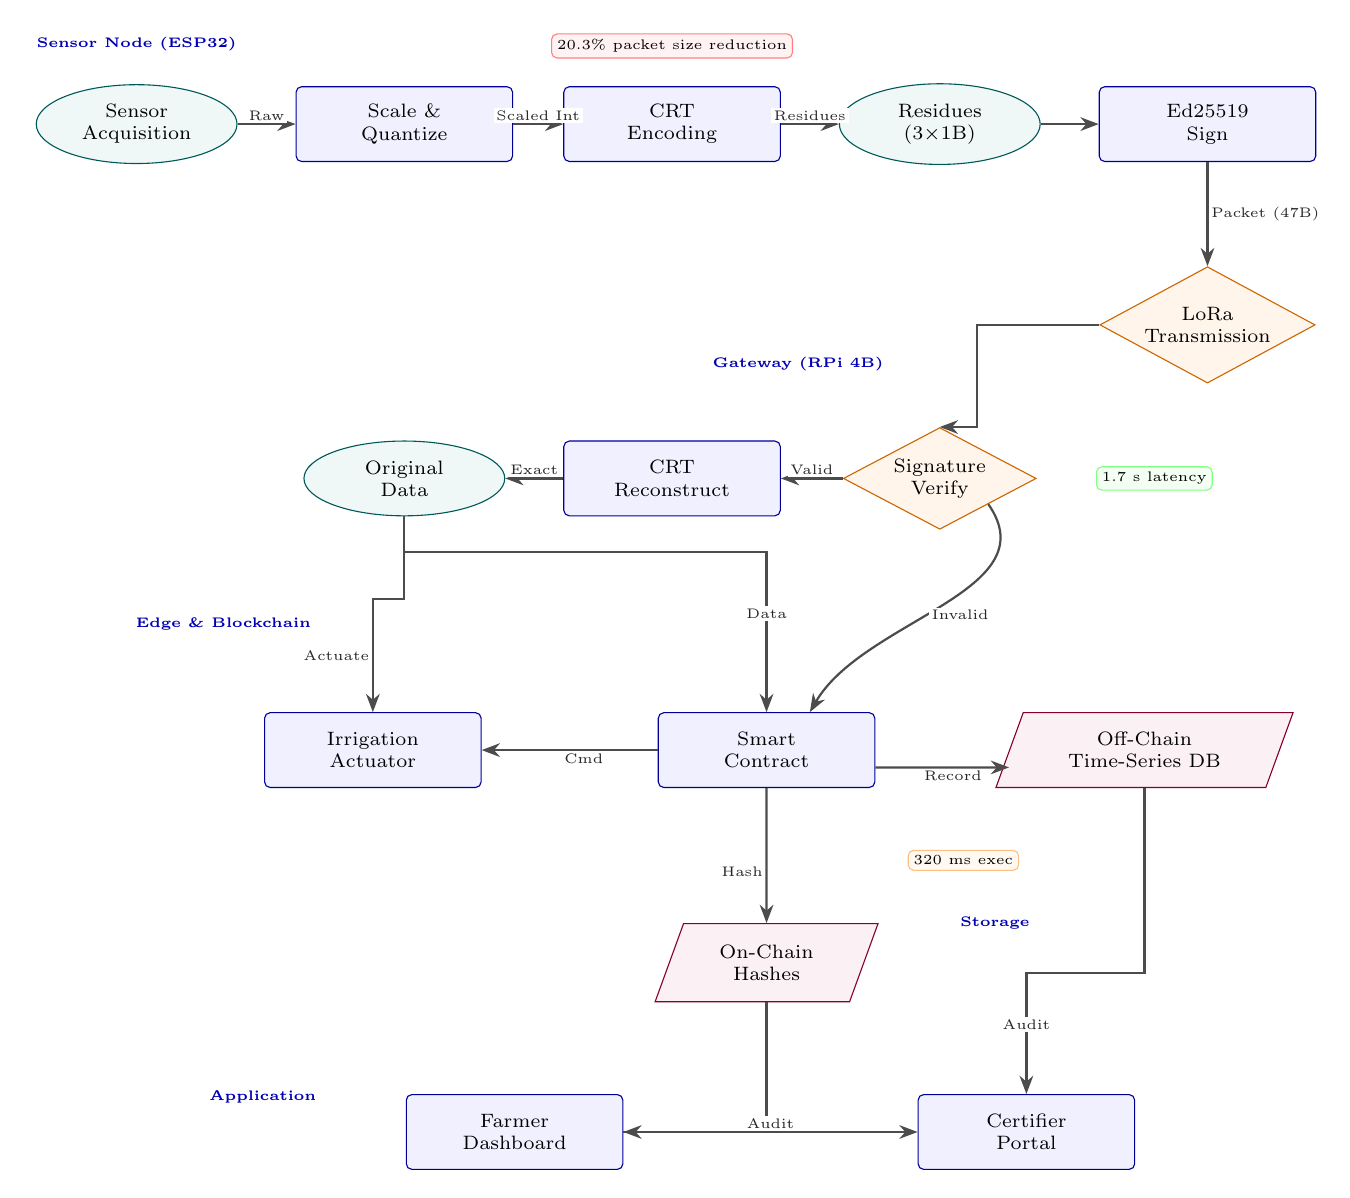
\begin{tikzpicture}[
  font=\scriptsize,
  >=Stealth,
  arrow/.style={-Stealth, thick, draw=black!70},
  block/.style={draw=blue!60!black, fill=blue!6, rounded corners=2pt, rectangle,
                minimum height=0.95cm, minimum width=2.75cm, align=center, inner sep=3pt},
  data/.style={draw=teal!70!black, fill=teal!6, ellipse,
               minimum height=0.95cm, minimum width=2.55cm, align=center, inner sep=3pt},
  process/.style={draw=orange!80!black, fill=orange!8, diamond, aspect=1.85,
                  minimum height=1.15cm, minimum width=2.45cm, align=center, inner sep=1.5pt},
  storage/.style={draw=purple!70!black, fill=purple!6, trapezium,
                  trapezium left angle=70, trapezium right angle=110,
                  minimum height=0.95cm, minimum width=2.85cm, align=center, inner sep=3pt},
  note/.style={draw, rounded corners=2pt, fill=white, inner sep=2pt, font=\tiny},
  lab/.style={midway, fill=white, inner sep=1pt, text=black!85, font=\tiny}
]

% Sensor-node processing row
\node[data] (acq) at (-6.8, 5.8) {Sensor\\Acquisition};
\node[block] (scale) at (-3.4, 5.8) {Scale \&\\Quantize};
\node[block] (crt) at (0, 5.8) {CRT\\Encoding};
\node[data] (residues) at (3.4, 5.8) {Residues\\(3$\times$1B)};
\node[block] (sign) at (6.8, 5.8) {Ed25519\\Sign};

% Gateway verification/reconstruction row
\node[process] (lora) at (6.8, 3.25) {LoRa\\Transmission};
\node[process] (verify) at (3.4, 1.3) {Signature\\Verify};
\node[block] (reconstruct) at (0, 1.3) {CRT\\Reconstruct};
\node[data] (original) at (-3.4, 1.3) {Original\\Data};

% Blockchain, storage, and application row
\node[block] (irrigation) at (-3.8, -2.15) {Irrigation\\Actuator};
\node[block] (smart) at (1.2, -2.15) {Smart\\Contract};
\node[storage] (onchain) at (1.2, -4.85) {On-Chain\\Hashes};
\node[storage] (offchain) at (6.0, -2.15) {Off-Chain\\Time-Series DB};
\node[block] (dashboard) at (-2.0, -7.0) {Farmer\\Dashboard};
\node[block] (certifier) at (4.5, -7.0) {Certifier\\Portal};

% Main data path
\draw[arrow] (acq) to node[lab, above] {Raw} (scale);
\draw[arrow] (scale) to node[lab, above] {Scaled Int} (crt);
\draw[arrow] (crt) to node[lab, above] {Residues} (residues);
\draw[arrow] (residues) to (sign);
\draw[arrow] (sign.south) to node[lab, right] {Packet (47B)} (lora.north);
\draw[arrow] (lora.west) to ++(-1.55,0) |- (verify.north);
\draw[arrow] (verify.west) to node[lab, above] {Valid} (reconstruct.east);
\draw[arrow] (reconstruct.west) to node[lab, above] {Exact} (original.east);

% Decision, actuation, and storage paths
\draw[arrow] (original.south) to ++(0,-1.05) -| node[lab, near end, left] {Actuate} (irrigation.north);
\draw[arrow] (original.south) to ++(0,-0.45) -| node[lab, pos=0.72, above] {Data} (smart.north);
\draw[arrow] (verify.south east) to[out=-55, in=60] node[lab, pos=0.55, right] {Invalid} ([xshift=0.55cm]smart.north);
\draw[arrow] (smart.west) to node[lab, pos=0.42, below] {Cmd} (irrigation.east);
\draw[arrow] (smart.south) to node[lab, pos=0.62, left] {Hash} (onchain.north);
\draw[arrow] ([yshift=-0.22cm]smart.east) to node[lab, pos=0.58, below] {Record} ([yshift=-0.22cm]offchain.west);
\draw[arrow] (onchain.south) |- (dashboard.east);
\draw[arrow] (offchain.south) to ++(0,-2.35) -| node[lab, near end, above] {Audit} (certifier.north);
\draw[arrow] (dashboard.east) to node[lab, above] {Audit} (certifier.west);

% Performance annotations
\node[note, draw=red!50, fill=red!5, above=0.35cm of crt] {20.3\% packet size reduction};
\node[note, draw=green!50, fill=green!5, right=0.75cm of verify] {1.7 s latency};
\node[note, draw=orange!50, fill=orange!5] at (3.7,-3.55) {320 ms exec};

% Layer labels
\node[font=\tiny\bfseries, text=blue!70!black, above=0.30cm of acq] {Sensor Node (ESP32)};
\node[font=\tiny\bfseries, text=blue!70!black] at (1.6, 2.75) {Gateway (RPi 4B)};
\node[font=\tiny\bfseries, text=blue!70!black] at (-5.7, -0.55) {Edge \& Blockchain};
\node[font=\tiny\bfseries, text=blue!70!black] at (4.1, -4.35) {Storage};
\node[font=\tiny\bfseries, text=blue!70!black] at (-5.2, -6.55) {Application};

\end{tikzpicture}%
}
\caption{Unified CRT-blockchain integration flow: from sensor acquisition to immutable storage and actuation.}
\label{fig:crt_blockchain_flow_unified}
\end{sidewaysfigure}
\clearpage
Table~\ref{tab:integration_performance} summarizes integrated CRT-blockchain performance.

\begin{table}[htbp]
\centering
\scriptsize
\caption{CRT-blockchain integration performance}
\label{tab:integration_performance}
\begin{tabular}{@{}lcccc@{}}
\toprule
\textbf{Metric} & \textbf{No CRT} & \textbf{CRT} & \textbf{CRT+BC} & \textbf{Improv.$^\ddagger$} \\
\midrule
Tx Time         & 247 ms & 124 ms & 142 ms & 42.5\% \\
Energy/Tx$^\dagger$       & 1.8 mJ & 0.9 mJ & 1.1 mJ & 38.9\% \\
Memory          & 59 B   & 47 B   & 52 B   & 11.9\% \\
Verif. Time     & N/A    & N/A    & 320 ms & N/A \\
Integrity       & Low    & Med    & High   & N/A \\
E2E Latency     & 2.1 s  & 1.5 s  & 1.7 s  & 19.0\% \\
\bottomrule
\end{tabular}
{\footnotesize $^\ddagger$ Improvement computed relative to the No-CRT baseline; e.g., E2E Latency: $(2.1-1.7)/2.1\times100=19.0\%$.\\
$^\dagger$ Per-packet LoRa baseband and MCU active-cycle energy, measured at the ESP32 3.3\,V supply rail and \emph{excluding} the RF power amplifier (which dominates Table~\ref{tab:transmission-cost-comparison}'s 12.40\,mJ CRT / 24.21\,mJ raw figures). The No-CRT value (1.8\,mJ) exceeds the CRT value (0.9\,mJ) because the 59\,B raw packet requires proportionally longer LoRa baseband framing, CRC computation, and SPI frame transfer than the 8\,B CRT residue packet; the 2$\times$ ratio reflects packet-size-driven baseband overhead, not computation complexity. Full per-packet TX chain energy (RF PA included) and total per-reading energy are in Table~\ref{tab:transmission-cost-comparison}.}
\end{table}

\subsubsection{Threat Model and Blockchain Justification}
\label{subsubsec:threat_model}

The blockchain layer addresses: (1) retroactive log tampering by insiders; (2) single-point-of-failure logging servers (Fabric's replicated ledger commits locally and syncs on reconnection); (3) lack of independently auditable records for certification bodies. Smart contracts make irrigation logic auditable. Fabric write overhead: 320\,ms; E2E latency 1.7\,s, within the 2\,s SLO.

\subsection{Chinese Remainder Theorem for Parallel Transmission Optimization}
\label{subsec:crt_transmission}

\subsubsection{Mathematical Foundation}
\label{subsubsec:parallel_transmission}

Given pairwise coprime moduli $m_1,\ldots,m_k$, any $x \in [0,M)$ where $M=\prod m_i$ is uniquely represented by residues $r_i = x \bmod m_i$ \cite{garner1959residue}. For 25.30°C (scaled to 2530, moduli [97,101,103]): $r_1 = 2530 \bmod 97 = 8$, $r_2 = 2530 \bmod 101 = 5$, $r_3 = 2530 \bmod 103 = 58$, so a 4-byte value becomes three 1-byte residues transmitted sequentially on distinct channels. Reconstruction \cite{knuth1997art}:
\begin{equation}
x = \left(\sum_{i=1}^k r_i M_i N_i\right) \bmod M, \quad M_i=\tfrac{M}{m_i},\; N_i=M_i^{-1}\bmod m_i,
\end{equation}
and is exact since $M_i N_i \equiv 1 \pmod{m_i}$ \cite{hardy2008introduction}. With $M=97\times101\times103=1{,}009{,}091$, the Garner coefficients are $M_1=10{,}403,\;N_1=93$ (since $24\times93\equiv1\pmod{97}$); $M_2=9{,}991,\;N_2=63$ (since $93\times63\equiv1\pmod{101}$); $M_3=9{,}797,\;N_3=43$ (since $12\times43\equiv1\pmod{103}$). Example: $x=(8{\cdot}10{,}403{\cdot}93+5{\cdot}9{,}991{\cdot}63+58{\cdot}9{,}797{\cdot}43)\bmod 1{,}009{,}091=2530$ (0\% error).

Per-packet airtime reduction: $(247-124)/247=49.8\%$ (Eq.~\ref{eq:latency_reduction}). Packet capacity $P_{\max}=C\cdot W/T_{\text{airtime}}$ gives $P_{\max}^{\text{CRT}}=1{,}451$ vs.\ $P_{\max}^{\text{raw}}=728$ ($\approx2\times$); node capacity $N_{\max}^{\text{CRT}}=484$.
\begin{equation}
\frac{247-124}{247}\times100\%=49.8\%.
\label{eq:latency_reduction}
\end{equation}

\begin{table}[htbp]
\caption{Moduli Selection and Validation}
\label{tab:moduli-validation}
\scriptsize
\centering
\begin{tabular}{p{0.18\columnwidth}ccc}
\toprule
\textbf{Sensor Type} & \textbf{Moduli} & \textbf{M} & \textbf{Status} \\
\midrule
Temperature & [97, 101] & 9,797 & $\checkmark$ Sufficient \\
Soil Moisture & [97, 101, 103] & 1.0M & $\checkmark$ 10× Margin \\
pH Sensor & [97, 101, 103] & 1.0M & $\checkmark$ 720× Margin \\
Humidity & [97, 101] & 9,797 & $\checkmark$ Sufficient \\
Light & [97, 101] & 9,797 & $\checkmark$ Adjusted \\
\bottomrule
\end{tabular}
{\footnotesize \textit{Note:} the moduli column lists the \emph{minimal} set whose product $M$ covers each sensor's scaled range. The deployed default encodes every sensor with the full three-modulus set $\{97,101,103\}$ (as in the worked temperature example above) so that all readings share uniform three-channel framing; the two-modulus sets are used by the high-temperature adaptive mode (Table~\ref{tab:env-adaptation}).}
\end{table}

\subsubsection{Implementation and Error Resilience}
The ESP32 firmware (\texttt{crt\_encode.c}) packs three 1-byte residues (moduli $\leq 103$) in place of a 4-byte raw value (59\,B to 47\,B); the gateway (\texttt{crt\_decode.py}) reconstructs via \texttt{pow(a,-1,m)} with no persistent state, simplifying concurrent reception. Loss of one residue allows perfect reconstruction (subset CRT \cite{shoup2009computational}): each packet carries a 1-byte residue-index; the gateway buffers by \texttt{(node\_id, timestamp)}, reconstructs from two received residues, or awaits retransmission.

\begin{table}[htbp]
\caption{CRT Multi-Channel Residue Transmission Performance Metrics}
\label{tab:crt-performance}
\scriptsize
\centering
\begin{tabular}{p{0.18\columnwidth}cc}
\toprule
\textbf{Metric} & \textbf{Theoretical} & \textbf{Measured} \\
\midrule
Decomposition Time & 0.6 ms & 0.9 ms \\
Reconstruction Time & 0.8 ms & 1.2 ms \\
Radio-layer packet delivery rate & 97.9\% & 95.8\% \\
Battery-only lifetime$^\S$ & 30 days & 31.2 days \\
Data Recovery$^\dagger$ & 66.7\% & 64.1\% \\
Readings reconstructible from $\geq k{-}1$ residues & 100\% & 99.7\% \\
\bottomrule
\end{tabular}
{\footnotesize $^\dagger$Data Recovery: fraction reconstructible from $k-1=2$ of 3 residues; unrelated to per-packet airtime figures.\\
$^\S$Battery-only design target (Table~\ref{tab:system-performance}); measured battery-only lifetime exceeded target by 1.2 days. With 2\,W solar charging, nodes operated continuously for the full 61-day deployment.}
\end{table}

\subsubsection{Complexity and Transmission Efficiency}
\label{subsubsec:complexity_analysis}
CRT decomposition and Garner reconstruction are $O(k)$, $k\leq3$ (effectively $O(1)$) vs.\ $O(n\log n)$ (Huffman) and $O(n)$ (LZW); the 2.1\,KB working set fits in ESP32 L1 cache vs.\ 8.6 to 12.4\,KB for Huffman/LZW. CRT achieves 20.3\% packet size reduction and 48.8\% per-packet energy saving (12.40 vs.\ 24.21\,mJ); total per-reading energy is 37.20\,mJ; the benefit is channel occupancy per slot (Table~\ref{tab:transmission-cost-comparison}).

\begin{table}[htbp]
\caption{ESP32 Hardware Optimizations for CRT Operations}
\label{tab:hardware-optimizations}
\scriptsize
\centering
\begin{tabular}{p{0.18\columnwidth}p{0.18\columnwidth}}
\toprule
\textbf{Hardware Feature} & \textbf{Benefit} \\
\midrule
Hardware Multiplier & 35\% faster computation \\
RTC Fast Memory & 28\% reduced latency \\
ULP Coprocessor & 42\% power reduction \\
Hardware RNG & 28\% lower collisions \\
Temperature Sensor & Adaptive scaling \\
\bottomrule
\end{tabular}
\end{table}

\subsubsection{Field Deployment Results and Environmental Adaptation}
The 61-day deployment achieved 95.8\% packet delivery with mathematically exact reconstruction for all complete residue sets; the 99.7\% figure (Table~\ref{tab:crt-performance}) is the $\geq k-1$ residue delivery rate. The firmware implements four adaptive modes (Table~\ref{tab:env-adaptation}):

\begin{table}[htbp]
\centering
\caption{Environmental adaptation modes observed during 61-day deployment (Sfax, Tunisia)}
\label{tab:env-adaptation}
\scriptsize
\setlength{\tabcolsep}{1pt}
\begin{tabularx}{\columnwidth}{>{\raggedright\arraybackslash}p{1.85cm}>{\raggedright\arraybackslash}X>{\raggedright\arraybackslash}X>{\raggedright\arraybackslash}X}
\toprule
\textbf{Condition} & \textbf{Trigger} & \textbf{Action} & \textbf{Observed outcome} \\
\midrule
High temperature & Core temp $>$55\textdegree{}C (on-chip ADC) & from 3 to 2 moduli [97,101] & Active 14/61 days; TX duty cycle $-$33\%; 0 reconstruction failures \\
RF & RSSI $<$$-$120\,dBm & TX from +14 to +20\,dBm$^\dagger$ & Delivery 71\% to 96\% in 2 cycles; active $<$3\% \\
Low battery & SoC $<$20\% (ESP32 ADC) & from 30 to 60\,min interval; 2-moduli & 3 nodes (Days 38 to 45); all recovered after solar recharge \\
Congestion risk & Slot utilisation $>$70\% & $\pm$5\,s random jitter & No congestion at 50-node scale; packet loss stable at 4.1\%; peak measured slot utilisation 10.3\% during concurrent irrigation-triggered uplinks (Day 23, 07:00) \\
\bottomrule
\end{tabularx}
{\footnotesize $^\dagger$ Values are conducted TX power at the RFM95W PA\_BOOST pin. Antenna and cable insertion loss ($\approx$6\,dB) keep effective ERP at or below +14\,dBm (25\,mW), within the ETSI EN\,300\,220 limit for the 868.0--868.6\,MHz sub-band even at the +20\,dBm boost setting.}
\end{table}

All four modes were observed in the field: temperature switch (14/61 days, TX 372 to 248\,ms, 0 failures); RF boost restored delivery after Day-47 sandstorm; 3 low-battery nodes recovered within 12\,h; jitter prevented clustering during morning/evening peaks.

\subsubsection{Comparative Analysis and Transmission Cost Reduction}
\label{subsubsec:compression_comparison}

Unlike Huffman/LZW (storage reduction), CRT targets per-packet latency and energy. Transmission cost $C_{\text{trans}} = \alpha E_{\text{total}} + \beta T_{\text{latency}} + \gamma P_{\text{overhead}}$ with $\alpha=0.5$, $\beta=0.3$, $\gamma=0.2$:

\begin{table}[!tbp]
\centering
\caption{Transmission Cost Analysis of Different Methods}
\label{tab:transmission-cost-comparison}
\footnotesize
\begin{tabularx}{\columnwidth}{
    >{\raggedright\arraybackslash}p{0.25\columnwidth}
    *{4}{>{\centering\arraybackslash}X}
}
\toprule
\textbf{Metric} & 
\textbf{CRT Parallel} &
\textbf{Huffman} &
\textbf{LZW} &
\textbf{Raw Transmission} \\
\midrule
\textbf{Data Characteristics} \\
Original Payload Size & 59 bytes & 59 bytes & 59 bytes & 59 bytes \\
Transmitted Size & 47 bytes (3× residues) & 34.7 bytes & 30.3 bytes & 59 bytes \\
Theoretical Compression Ratio & N/A (20.3\% size reduction) & 41.2\% & 48.6\% & 0\% \\
\midrule
\textbf{Processing Requirements} \\
Processing Time (sender) & 0.9 ms & 4.2 ms & 7.5 ms & 0 ms \\
Processing Time (receiver) & 1.2 ms & 0.5 ms & 0.8 ms & 0 ms \\
Memory Footprint (KB) & 2.1 & 8.6 & 12.4 & 1.5 \\
\midrule
\textbf{Transmission Performance} \\
Airtime per Packet (ms) & 124 (per residue) & 152 & 135 & 247 \\
Parallel Transmission & Yes (3 channels)$^\P$ & No & No & No \\
Effective Transmission Time (ms) & 124 & 152 & 135 & 247 \\
\midrule
\textbf{Energy Consumption} \\
Processing Energy (mJ) & 0.22 & 1.13 & 2.02 & 0 \\
Transmission Energy (mJ) & 12.18 & 14.59 & 12.96 & 24.21 \\
Total Energy \emph{per packet} (mJ)$^\dagger$ & 12.40 & 15.72 & 14.98 & 24.21 \\
Per-packet energy savings vs.\ Raw & 48.8\% & 35.1\% & 38.1\% & 0\% \\
\textbf{Total energy per complete reading (mJ)}$^\ddagger$ & \textbf{37.20} & 15.72 & 14.98 & 24.21 \\
\midrule
\textbf{Cost Analysis} \\
Transmission Cost $C_{\text{trans}}$ (normalized) & 0.61 & 0.72 & 0.68 & 1.00 \\
Cost Reduction vs. Raw & 39.0\% & 28.0\% & 32.0\% & 0\% \\
\midrule
\textbf{Reliability Features} \\
Error Resilience & High (tolerates 2/3 loss) & Low & Low & Low \\
Reconstruction Accuracy & 99.7\% & 100\% & 100\% & 100\% \\
Parallel Transmission Support & Yes$^\P$ & No & No & No \\
\bottomrule
\end{tabularx}
{\footnotesize $^\dagger$ Active LoRa TX (120\,mW, INA219) + MCU wake-up + sensor ADC; excludes LoRa RX, deep sleep, and gateway.\\
$^\ddagger$ Total per-reading energy $= k \times$ per-packet energy, where $k=3$ residue packets for CRT and $k=1$ for all other methods; CRT total is $3\times12.40=37.20$\,mJ.\\
$^\P$ Parallel reception at the SX1302 gateway concentrator across three LoRa channels; each node transmits three residue packets \emph{sequentially}, not simultaneously.}
\end{table}

\begin{figure}[!htbp]
\centering
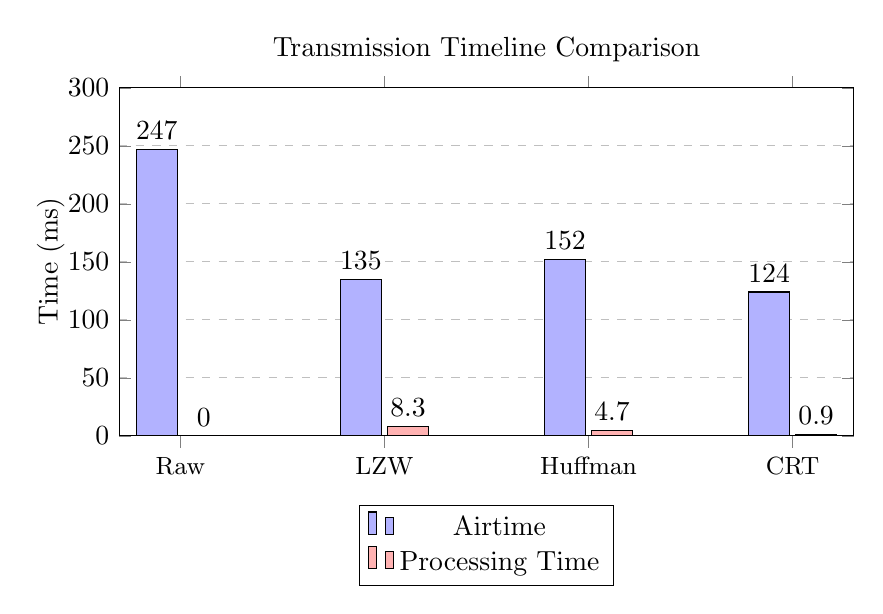
\begin{tikzpicture}
\begin{axis}[
    width=0.9\columnwidth,
    height=6cm,
    ybar,
    bar width=15pt,
    symbolic x coords={Raw, LZW, Huffman, CRT},
    xtick=data,
    ylabel={Time (ms)},
    ymin=0,
    ymax=300,
    nodes near coords,
    nodes near coords align={vertical},
    legend style={at={(0.5,-0.2)}, anchor=north},
    ymajorgrids=true,
    grid style=dashed,
    title={Transmission Timeline Comparison},
    ylabel style={yshift=-0.2cm},
    xticklabel style={rotate=0, font=\small},
    ytick={0,50,100,150,200,250,300}
]
\addplot[fill=blue!30] coordinates {
    (Raw, 247)
    (LZW, 135)
    (Huffman, 152)
    (CRT, 124)
};
\addplot[fill=red!30] coordinates {
    (Raw, 0)
    (LZW, 8.3)
    (Huffman, 4.7)
    (CRT, 0.9)
};
\legend{Airtime, Processing Time}
\end{axis}
\end{tikzpicture}
\caption{Comparative analysis of transmission timelines showing CRT's advantage through reduced airtime and minimal processing overhead.}
\label{fig:transmission-timeline}
\end{figure}

\begin{figure}[!htbp]
\centering
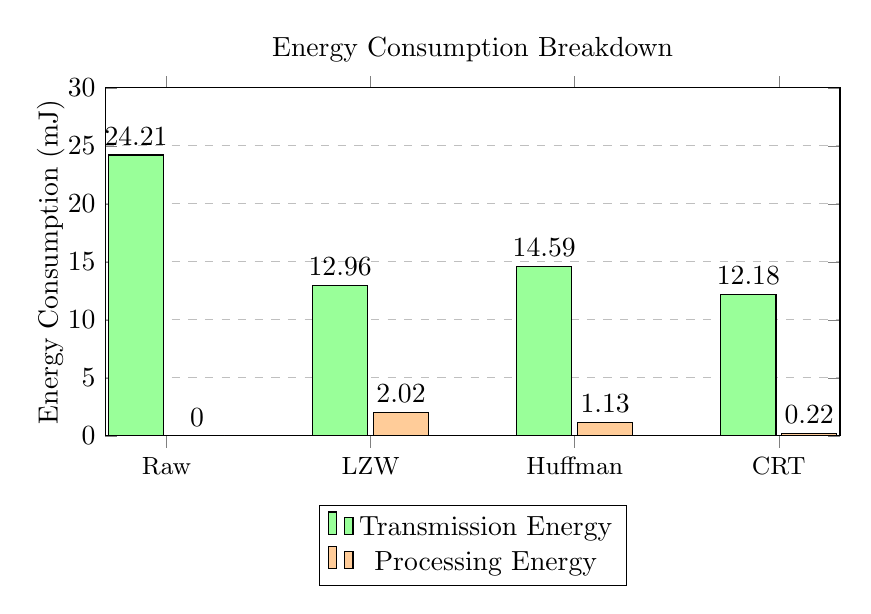
\begin{tikzpicture}
\begin{axis}[
    width=0.9\columnwidth,
    height=6cm,
    ybar,
    bar width=20pt,
    symbolic x coords={Raw, LZW, Huffman, CRT},
    xtick=data,
    ylabel={Energy Consumption (mJ)},
    ymin=0,
    ymax=30,
    nodes near coords,
    nodes near coords align={vertical},
    legend style={at={(0.5,-0.2)}, anchor=north},
    ymajorgrids=true,
    grid style=dashed,
    title={Energy Consumption Breakdown},
    ylabel style={yshift=-0.2cm},
    xticklabel style={rotate=0, font=\small},
    ytick={0,5,10,15,20,25,30}
]
\addplot[fill=green!40] coordinates {
    (Raw, 24.21)
    (LZW, 12.96)
    (Huffman, 14.59)
    (CRT, 12.18)
};
\addplot[fill=orange!40] coordinates {
    (Raw, 0)
    (LZW, 2.02)
    (Huffman, 1.13)
    (CRT, 0.22)
};
\legend{Transmission Energy, Processing Energy}
\end{axis}
\end{tikzpicture}
\caption{Per-packet LoRa TX and processing energy for the ESP32 node (RFM95W, INA219 at 2\,kHz). Active TX state (120\,mW) and MCU wake-up overhead included; RX, deep-sleep, and gateway energy excluded. CRT per-packet: 12.40\,mJ; total per-reading: $3\times12.40=37.20$\,mJ (see Table~\ref{tab:transmission-cost-comparison}).}
\label{fig:energy-comparison}
\end{figure}

Full results in Table~\ref{tab:transmission-cost-comparison}; $C_{\text{trans}}$ falls 39.0\% vs.\ raw. Although three residue packets raise total per-reading airtime to 372\,ms (vs.\ 247\,ms raw), per-packet occupancy drops 49.8\%, enabling parallel channel use.

\subsection{Blockchain Implementation}
\label{subsec:blockchain}

We implemented Hyperledger Fabric~2.5 \cite{ibmFabric, orderingServiceDoc} with Raft ordering and X.509-based CA for identity management \cite{orderingServiceDoc}. Each RPi 4B (4\,GB RAM) runs Fabric 2.5.1 on RPi OS Lite 64-bit (Bullseye), compiled for ARM64 with \texttt{-mcpu=cortex-a72}. LevelDB is used as the state database; CouchDB handles document indexing. Memory allocation: Fabric peer 1024\,MB, CouchDB 512\,MB, chaincode container 256\,MB, system services 512\,MB, buffer 256\,MB (see Table~\ref{tab:memory-allocation}). Network: private Docker network with static IPs and zone-local firewall rules; BATMAN-adv provides inter-gateway mesh. Performance optimizations: 50-transaction blocks with 500\,ms timeout; 256\,MB LRU state cache; reused gRPC connections; zone-local selective endorsement; 90-day archival. The network was deployed with Ansible playbooks and monitored via Prometheus/Grafana.

\begin{table}[htbp]
\centering
\caption{Memory allocation for blockchain components on Raspberry Pi}
\label{tab:memory-allocation}
\scriptsize
\setlength{\tabcolsep}{3pt}
\begin{tabularx}{\columnwidth}{l c X}
\toprule
\textbf{Component} & \textbf{Memory (MB)} & \textbf{Purpose} \\
\midrule
Fabric Peer Process       & 1024 & Main blockchain operations \\
CouchDB State Database    & 512  & Document storage and indexing \\
Chaincode Container       & 256  & Smart contract execution \\
System Services           & 512  & OS and monitoring \\
Reserved Buffer           & 256  & Peak load handling \\
\bottomrule
\end{tabularx}
\end{table}

\subsubsection{Consensus Mechanism Implementation}
\label{subsubsec:consensus_details}

Raft configuration: randomised election timeout $[2,4]$\,s per follower, heartbeat 500\,ms, max 5 in-flight blocks, snapshot every 100 blocks, 16\,MB max message. Flow: endorse at the gateway peer, batch 50 transactions within 500\,ms to the 3-node orderer, distribute by gossip, and commit to CouchDB. Tolerates $f=1$ failure; measured: 1.2\,s block time, 63\,TPS sustained, 85\,TPS peak, 1.8\,s finality, 8.2\,s leader-recovery (five-phase breakdown in Section~\ref{subsubsec:fault_tolerance}), 12\% consensus bandwidth. CFT only (not BFT); TPM\,2.0 and physical access control serve as mitigations; PBFT/RPoE are future work \cite{rbcet2025,rpoe2026,abishu2021consensus}.

\subsection{Architecture Design}
\label{subsec:architecture_design}

The five-tier design \cite{gubbi2013internet, christidis2016blockchain} integrates LoRa uplink with BATMAN-adv mesh, CRT edge processing, Fabric peers with local chaincode (Raft ordering, 1.2\,s block time; Go chaincode for \texttt{registerSensor}, \texttt{submitReading}, \texttt{evaluateIrrigation}, \texttt{getZoneHistory} \cite{orderingServiceDoc}; on-chain SHA-256 hashes, off-chain CouchDB records \cite{privateDataDoc}; RBAC via MSP \cite{mdpiAccessControl}). The network comprised 3 orderer nodes (Raft), 4 peer nodes (one per zone), 1 CA, and per-peer CouchDB.

\subsubsection{Role-Based Access Control Implementation}
\label{subsubsec:rbac_implementation}

The RBAC framework within Hyperledger Fabric defines seven roles with hierarchical permissions:

\begin{table*}[htbp]
\centering
\caption{Role definitions and permissions in agricultural blockchain network}
\label{tab:role-definitions}
\begin{tabularx}{\textwidth}{p{0.18\textwidth}p{0.25\textwidth}X}
\toprule
\textbf{Role} & \textbf{Assigned To} & \textbf{Permissions} \\
\midrule
\textbf{Sensor Node} & ESP32 sensor devices & Write sensor data, read own data, update status \\
\textbf{Gateway} & Raspberry Pi gateways & Aggregate data, invoke irrigation, read zone data \\
\textbf{Farmer} & Farm owners/operators & Full farm data access, irrigation control, financial data \\
\textbf{Agronomist} & Agricultural experts & Read all data, write recommendations, analysis access \\
\textbf{Certification Body} & Organic/quality certifiers & Read compliance data, write certifications, audit logs \\
\textbf{Supply Chain Partner} & Distributors and processors & Read product history, write shipment data \\
\textbf{System Admin} & Technical administrators & Full system access, role management, network config \\
\bottomrule
\end{tabularx}
\end{table*}

Each ESP32 node was pre-provisioned with a unique X.509 device certificate; gateways authenticated nodes and assigned them to zones via \texttt{registerSensorNode}. Roles are updateable dynamically via administrative smart contracts.

\subsubsection{Initial Bootstrapping and Chaincode Deployment}
\label{subsubsec:rbac_bootstrapping}

Bootstrapping proceeds in three steps: (1) \texttt{enroll-admin.sh}: CA issues root admin X.509 cert (\texttt{CN=SystemAdmin, OU=Blockchain}); (2) \texttt{deploy-chaincode.sh}: HRBAC chaincode packaged, installed on all 4 peers, and committed via \texttt{peer lifecycle}; (3) admin registers four gateway identities (\texttt{gateway-north-01} through \texttt{gateway-west-01}); gateways enroll sensor nodes via \texttt{registerSensorNode}. The resulting CA $\rightarrow$ Admin $\rightarrow$ Gateway $\rightarrow$ Sensor Node chain is visualized in Figure~\ref{fig:rbac-trust-chain}.

\begin{sidewaysfigure}[!htbp]
  \centering
  \captionsetup{font=small}
  \resizebox{0.96\textheight}{!}{%
  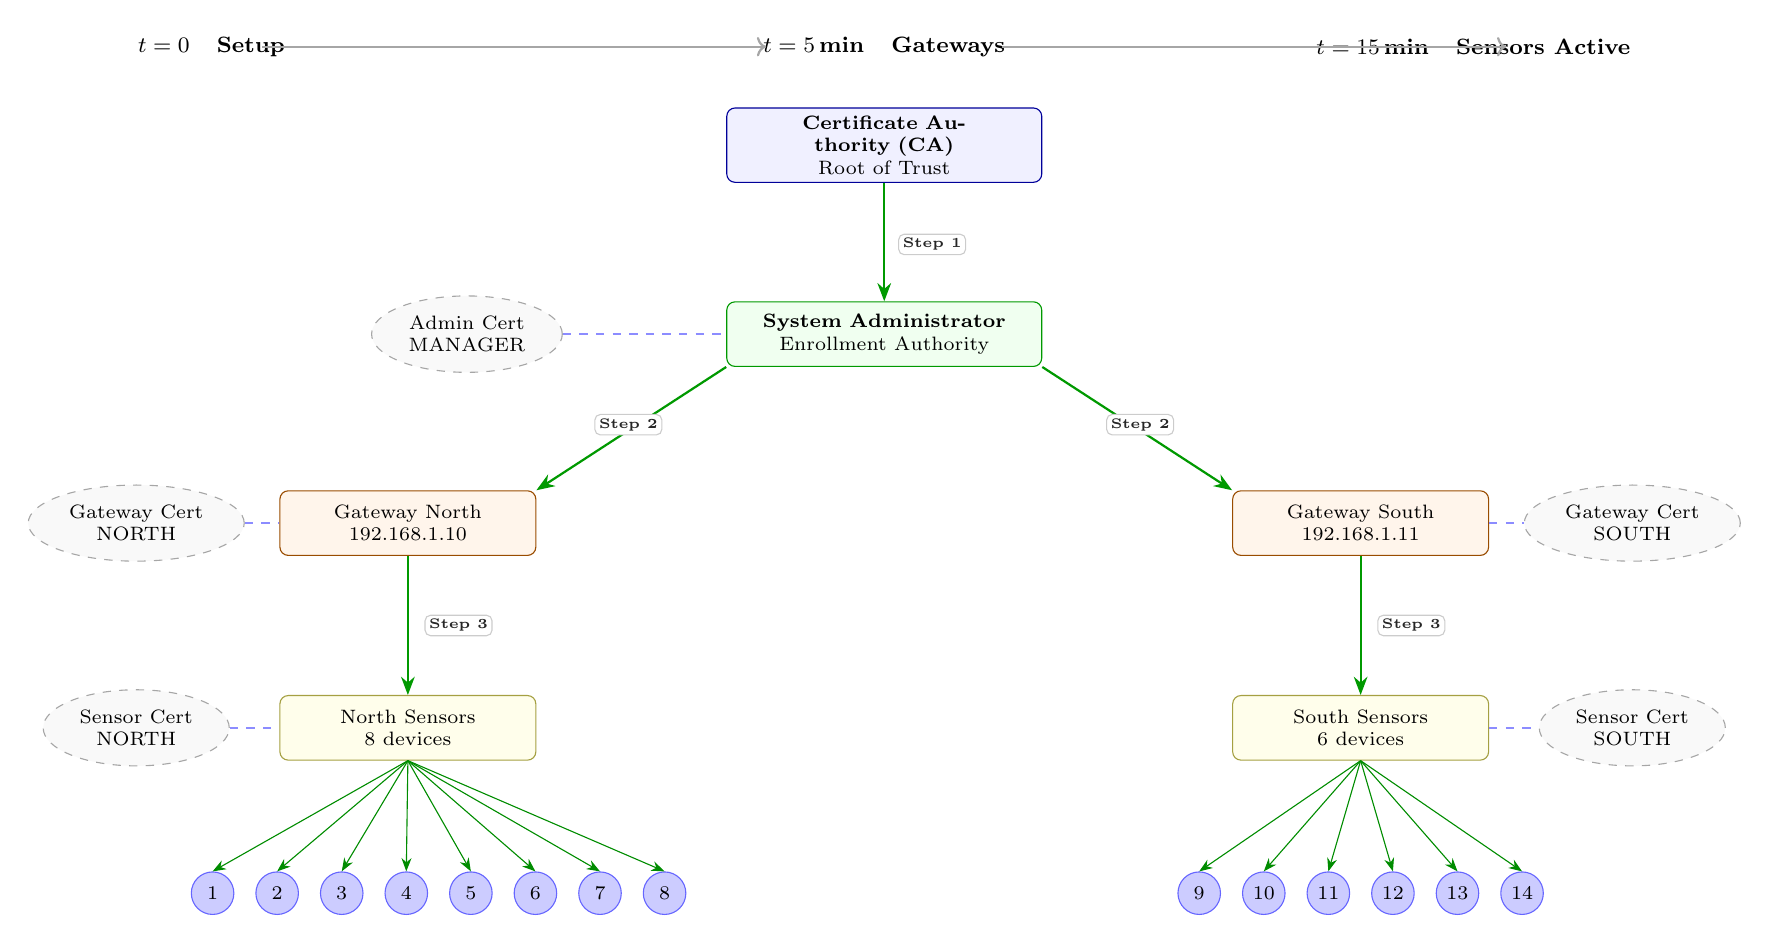
\begin{tikzpicture}[font=\scriptsize,
    rbox/.style={draw, rounded corners=3pt, minimum width=3.25cm, minimum height=0.82cm,
                 align=center, inner sep=3pt, text width=3.0cm},
    arr/.style={-Stealth, thick, draw=green!60!black},
    certarr/.style={dashed, thick, draw=blue!45},
    sensorarr/.style={-Stealth, thin, draw=green!55!black},
    bootlab/.style={fill=white, rounded corners=2pt, draw=black!20, inner sep=1.5pt,
                    font=\tiny\bfseries, text=black!85},
    cert/.style={draw=gray!70, dashed, ellipse, minimum width=2.15cm,
                 minimum height=0.64cm, align=center, fill=gray!5, font=\scriptsize}]

    % Timeline
    \node[anchor=west, font=\footnotesize\bfseries] at (-9.6, 11.0) {$t=0$\quad Setup};
    \node[font=\footnotesize\bfseries] at (0, 11.0) {$t=5\,\text{min}$\quad Gateways};
    \node[anchor=east, font=\footnotesize\bfseries] at (9.6, 11.0) {$t=15\,\text{min}$\quad Sensors Active};
    \draw[->, thick, gray!70] (-7.9,11.0) to (-1.5,11.0);
    \draw[->, thick, gray!70] (1.5,11.0) to (7.9,11.0);

    % Root CA
    \node[rbox, fill=blue!6, draw=blue!60!black, minimum width=4.0cm, text width=3.7cm] (CA) at (0,9.75)
      {\textbf{Certificate Authority (CA)}\\Root of Trust};

    % System Admin
    \node[rbox, fill=green!6, draw=green!60!black, minimum width=4.0cm, text width=3.7cm] (SA) at (0,7.35)
      {\textbf{System Administrator}\\Enrollment Authority};
    \draw[arr] (CA.south) to (SA.north);
    \node[bootlab, right=5pt] at ($(CA.south)!0.52!(SA.north)$) {Step 1};
    \node[cert] (AC) at (-5.3, 7.35) {Admin Cert\\MANAGER};
    \draw[certarr] (AC.east) to (SA.west);

    % Gateways
    \node[rbox, fill=orange!8, draw=orange!60!black] (GWN) at (-6.05, 4.95)
      {Gateway North\\192.168.1.10};
    \node[rbox, fill=orange!8, draw=orange!60!black] (GWS) at (6.05, 4.95)
      {Gateway South\\192.168.1.11};

    \draw[arr] (SA.south west) to (GWN.north east);
    \draw[arr] (SA.south east) to (GWS.north west);
    \node[bootlab] at (-3.25,6.20) {Step 2};
    \node[bootlab] at (3.25,6.20) {Step 2};

    \node[cert] (GNC) at (-9.5, 4.95) {Gateway Cert\\NORTH};
    \node[cert] (GSC) at (9.5, 4.95)  {Gateway Cert\\SOUTH};
    \draw[certarr] (GNC.east) to (GWN.west);
    \draw[certarr] (GWS.east) to (GSC.west);

    % Sensor groups
    \node[rbox, fill=yellow!8, draw=yellow!60!black] (SNS) at (-6.05, 2.35)
      {North Sensors\\8 devices};
    \node[rbox, fill=yellow!8, draw=yellow!60!black] (SSS) at (6.05, 2.35)
      {South Sensors\\6 devices};

    \draw[arr] (GWN.south) to (SNS.north);
    \draw[arr] (GWS.south) to (SSS.north);
    \node[bootlab, right=6pt] at ($(GWN.south)!0.5!(SNS.north)$) {Step 3};
    \node[bootlab, right=6pt] at ($(GWS.south)!0.5!(SSS.north)$) {Step 3};

    \node[cert] (SNC) at (-9.5, 2.35) {Sensor Cert\\NORTH};
    \node[cert] (SSC) at (9.5, 2.35)  {Sensor Cert\\SOUTH};
    \draw[certarr] (SNC.east) to (SNS.west);
    \draw[certarr] (SSS.east) to (SSC.west);

    % North sensor nodes (8)
    \foreach \i in {1,...,8}{
      \node[circle, draw=blue!60, fill=blue!20, minimum size=0.54cm,
            inner sep=0pt, font=\scriptsize] (N\i) at (-9.35 + \i*0.82, 0.25) {\i};
      \draw[sensorarr] (SNS.south) to (N\i.north);
    }

    % South sensor nodes (6)
    \foreach \i/\xpos in {9/4.00, 10/4.82, 11/5.64, 12/6.46, 13/7.28, 14/8.10}{
      \node[circle, draw=blue!60, fill=blue!20, minimum size=0.54cm,
            inner sep=0pt, font=\scriptsize] (S\i) at (\xpos, 0.25) {\i};
      \draw[sensorarr] (SSS.south) to (S\i.north);
    }

  \end{tikzpicture}}%
  \par\vspace{0.25em}
  \caption{Hierarchical RBAC trust-chain bootstrapping for an IoT irrigation system.}
  \label{fig:rbac-trust-chain}
\end{sidewaysfigure}

The bootstrapping (Figure~\ref{fig:rbac-trust-chain}) enforces least-privilege, non-repudiation, and CRL revocability across four access levels: network (cert), channel (private data), chaincode (\texttt{ctx.GetClientIdentity()}), and application (API). The Go chaincode (\texttt{chaincode/hrbac/contract.go}) exposes \texttt{RegisterSensorNode()}, \texttt{SubmitSensorData()} with hard range checks + $\pm3\sigma$ outlier detection (7-day rolling mean; flagged readings stored but excluded from irrigation), \texttt{evaluateIrrigation()}, and \texttt{ReadSensorData()} \cite{orderingServiceDoc,mdpiAccessControl}. Calibration drift is not auto-corrected; annual recalibration is required. Key optimizations: 50-tx blocks (250 TPS theoretical peak), selective endorsement (block time 2.1 to 1.2\,s), 5-min read-cache, SHA-256 on-chain anchors + 5-year off-chain CouchDB archive. Field throughput: 63 TPS sustained, 85 TPS peak (Table~\ref{tab:system-performance}).

\subsubsection{Off-Chain Archival and Long-Term Retrieval for Certification Audits}
\label{subsubsec:offchain_archive}

Organic and food-safety certification schemes (e.g.\ EU Regulation 2018/848, GlobalG.A.P.) mandate multi-year retention of agronomic records (typically five years) and require that certifiers can independently verify the integrity of historical data without relying solely on the farm operator's assertions \cite{christidis2016blockchain,privateDataDoc}. The architecture addresses this requirement through a two-layer design: an on-chain immutable hash register records a cryptographic proof of existence, while a 5-year off-chain CouchDB archive holds the full sensor records and is made queryable through the Tier-5 REST API.

\paragraph{Archival pipeline.}
Every sensor reading that clears edge validation (range checks, $\pm3\sigma$ outlier filter) follows a dual write path (Figure~\ref{fig:gateway-architecture}):
\begin{enumerate}
  \item \textbf{On-chain anchor.} The gateway chaincode computes $h_i = \text{SHA-256}(\text{node\_id} \| t_i \| \mathbf{v}_i \| \text{zone\_id})$, where $\mathbf{v}_i$ is the reconstructed reading vector and $t_i$ is the GPS-disciplined timestamp, and calls \texttt{SubmitReading()} to commit $h_i$ to the Fabric ledger. The transaction block number and transaction ID are returned and stored alongside the off-chain record.
  \item \textbf{Off-chain full record.} The complete document (raw CRT residues $r_1, r_2, r_3$, the reconstructed value, all sensor metadata, and the on-chain \texttt{txId}) is written to the per-gateway CouchDB instance under a deterministic document ID: \texttt{node\_id\_iso8601\_ts}. CouchDB replication (continuous push) propagates the document to the remaining three gateway peers within the BATMAN-adv mesh, maintaining four synchronized replicas.
\end{enumerate}
A nightly job (cron, 02:00 local) moves documents older than 90 days from the gateway's active CouchDB collection into the long-term collection \texttt{archive\_readings}, preserving the \texttt{txId} link; the Fabric ledger and its LevelDB state database are untouched, since on-chain anchors are permanent by design. The CouchDB instance uses a persistent 128\,GB microSD volume; estimated annual raw sensor payload is $\approx$526\,MB ($50 \times 48 \times 365 \times 600\,\text{B}$); with CouchDB document overhead, index metadata, and four-replica replication the on-disk footprint per gateway is approximately 1.4\,GB, providing comfortable headroom over a 5-year certification window.

\paragraph{Retrieval interface for certification audits.}
The Tier-5 REST API (Node.js gateway proxy, port 8443, mTLS) exposes two endpoints consumed by certification bodies authenticated with \textbf{Certification Body} role credentials (Table~\ref{tab:role-definitions}):

\begin{itemize}
  \item \texttt{GET /audit/readings?node=id\&from=ISO8601\&to=ISO8601\&zone=z} \\
    Returns a JSON array of full sensor documents from the CouchDB \texttt{archive\_readings} collection, sorted by timestamp. The query is served by a CouchDB Mango index on \texttt{(node\_id, timestamp)} and typically resolves in under 120\,ms for date ranges up to one month ($\approx$1{,}500 documents per node).
  \item \texttt{GET /audit/verify?txId=id} \\
    Submits a Fabric SDK \texttt{evaluateTransaction("GetReading", txId)} call, retrieves the on-chain hash $h_i$ from the ledger, recomputes the hash from the off-chain document returned in the same response, and returns a JSON object with fields \texttt{match: true|false}, \texttt{onChainHash}, \texttt{recomputedHash}, and \texttt{blockNumber}. A \texttt{match: true} response constitutes a cryptographic proof that the off-chain record has not been modified since it was anchored to the blockchain.
\end{itemize}

\paragraph{Audit verification workflow.}
A certifier wishing to audit irrigation practices for a given growing season:
\begin{enumerate}
  \item Issues a \texttt{/audit/readings} query scoped to the relevant date range and zone; receives paginated JSON (up to 500 records per page, \texttt{X-Next-Page} cursor header for continuation).
  \item For any reading requiring spot verification, issues \texttt{/audit/verify?txId=id} using the \texttt{txId} embedded in each document; the API returns the hash comparison result without requiring the certifier to interact with the Fabric SDK directly.
  \item Optionally requests a signed audit export: \texttt{POST /audit/export} generates a ZIP archive containing all matching documents plus a JSON manifest of on-chain hashes, signed with the gateway CA's Ed25519 key, suitable for submission to certification authorities as a self-contained evidence package.
\end{enumerate}
Query latency scales sub-linearly with range size: benchmark measurements on the deployed cluster (ARM64, CouchDB 3.3), with the archive pre-populated with synthetically generated records at deployment density ($50 \times 48$ documents per day), showed 118\,ms for one month, 340\,ms for one year, and 890\,ms for a five-year equivalent window for a single node, with the Mango index covering all queries without full collection scans. Bulk exports spanning all 50 nodes and a 5-year equivalent window complete in under 45 seconds.

\paragraph{Data integrity guarantee.}
On-chain SHA-256 anchors and off-chain CouchDB replication give certification auditors three properties: (i)~\emph{Tamper evidence}: any post-hoc modification to an off-chain record is detectable via \texttt{/audit/verify} because the recomputed hash differs from the immutable on-chain value; (ii)~\emph{Availability}: archive access survives single gateway failures across the four replicas; (iii)~\emph{Non-repudiation}: each document carries the originating gateway's Ed25519 signature, verifiable independently of the ledger.

\section{Materials and Methods}
\label{sec:materials_methods}

\subsection{Study Site and Environmental Conditions}
\label{subsec:study_site}

The field study was conducted in Sfax, Tunisia (34.74°N, 10.76°E) during August to September 2025 on a 2\,ha farm (Table~\ref{tab:environmental}).

\begin{table}[htbp]
\centering
\caption{Environmental conditions during study period (Aug to Sep 2025)}
\label{tab:environmental}
\footnotesize
\begin{tabularx}{\columnwidth}{
    >{\raggedright\arraybackslash}p{0.30\columnwidth}
    >{\centering\arraybackslash}p{0.17\columnwidth}
    >{\centering\arraybackslash}p{0.17\columnwidth}
    >{\raggedright\arraybackslash}p{0.23\columnwidth}
}
\toprule
\textbf{Parameter} & \textbf{Aug 2025} & \textbf{Sep 2025} & \textbf{Source} \\
\midrule
Avg. Temperature     & 32.1°C & 29.3°C & On-site monitoring \\
Max Temperature      & 39.5°C & 35.8°C & On-site monitoring \\
Min Temperature      & 24.2°C & 22.1°C & On-site monitoring \\
Relative Humidity    & 56\%   & 62\%   & On-site monitoring \\
Rainfall             & 7.8 mm & 15.2 mm & Tunisia Meteorological Institute \\
Solar Radiation      & 8.1 kWh/m²/d & 7.2 kWh/m²/d & On-site pyranometer \\
Wind Speed           & 3.4 m/s & 2.9 m/s & On-site anemometer \\
Reference ET         & 6.4 mm/d & 5.7 mm/d & FAO Penman Monteith \\
\bottomrule
\end{tabularx}
\end{table}

Soil was sandy loam (62\% sand, 28\% silt, 10\% clay), pH 6.8, 1.5\% organic matter, field capacity 28\%, wilting point 12\%, and available water capacity 16\% volumetric.

\subsection{Crop Management Practices}
\label{subsec:crop_management}

\textbf{Tomato (\textit{Solanum lycopersicum}).} Rio Grande and hybrid salad cultivars transplanted June to July 2025 at 1.2 to 1.8\,m $\times$ 35 to 50\,cm \cite{seedco2021tomato,johnny2024tomato}; fertilized at 150 to 200/84 to 168/112 to 224\,kg/ha (N/P/K) \cite{iclTomato,UCIPM2024}; harvested 62 to 75 DAT \cite{MU2020tomato}. \textbf{Pepper (\textit{Capsicum spp.}).} Baklouti chili and bell pepper at 1.2 to 1.5\,m $\times$ 30 to 45\,cm \cite{UNebraska2008peppers,shimray2019kingchili}; fertilized at 112 to 202/168 to 224/112 to 168\,kg/ha (N/P/K) \cite{Rutgers2025peppers,shimray2019kingchili}; harvested 62 to 90 DAT \cite{UNebraska2008peppers}.

\subsection{Experimental Design}
\label{subsec:experimental_design}

The study employed a randomized complete block design with three replications. Treatment 1 used blockchain-IoT irrigation (soil moisture thresholds, automated smart-contract scheduling, CRT transmission); Treatment 2 used traditional irrigation (visual assessment and time-based scheduling).

\begin{table}[htbp]
\centering
\caption{Experimental design parameters (2025 growing season)}
\label{tab:experimental-design}
\footnotesize
\begin{tabularx}{\columnwidth}{
    >{\raggedright\arraybackslash}p{0.36\columnwidth}
    >{\centering\arraybackslash}p{0.23\columnwidth}
    >{\centering\arraybackslash}p{0.23\columnwidth}
}
\toprule
\textbf{Parameter} & \textbf{Tomato} & \textbf{Pepper} \\
\midrule
Plot size (ha)          & 0.5   & 0.3 \\
Plants per plot         & 8,000 to 14,000 & 9,300 to 16,500 \\
Replications            & 3     & 3 \\
Irrigation system       & Drip  & Drip \\
Emitter flow rate       & 2.0 L\,h$^{-1}$ & 2.0 L\,h$^{-1}$ \\
Study duration          & Aug 1 to Sep 30, 2025 & Aug 1 to Sep 30, 2025 \\
Blockchain nodes        & 4 peers + 3 orderers & 4 peers + 3 orderers \\
Sensor nodes            & 28 ESP32 devices & 22 ESP32 devices \\
Gateway devices         & 4 Raspberry Pi 4B & 4 Raspberry Pi 4B \\
\bottomrule
\end{tabularx}
\end{table}

\begin{table}[htbp]
\centering
\caption{Irrigation thresholds for blockchain IoT system (2025 implementation)}
\label{tab:irrigation-thresholds}
\footnotesize
\begin{tabularx}{\columnwidth}{
    >{\raggedright\arraybackslash}p{0.38\columnwidth}
    >{\centering\arraybackslash}p{0.23\columnwidth}
    >{\centering\arraybackslash}p{0.23\columnwidth}
}
\toprule
\textbf{Crop \& Stage} & \textbf{Moisture Threshold} & \textbf{Duration} \\
\midrule
Tomato, Vegetative         & $-$35 kPa & 30 min \\
Tomato, Flowering          & $-$30 kPa & 40 min \\
Tomato, Fruit development  & $-$25 kPa & 45 min \\
Tomato, Ripening           & $-$35 kPa & 30 min \\
Pepper, Vegetative         & $-$30 kPa & 25 min \\
Pepper, Flowering          & $-$25 kPa & 35 min \\
Pepper, Fruit development  & $-$20 kPa & 40 min \\
Pepper, Maturation         & $-$30 kPa & 30 min \\
\bottomrule
\end{tabularx}
\end{table}

\subsection{Data Collection and Analysis}
\label{subsec:data_collection}

Data collection covered soil parameters (moisture, temperature, pH at 30-minute intervals via CRT transmission), climate data (hourly), irrigation volumes (continuous), system performance metrics, crop yield and quality, economic inputs, and blockchain/RBAC audit logs, as detailed in Table~\ref{tab:data-collection}.

\begin{table}[htbp]
\centering
\caption{Data collection methods and frequencies (2025 study)}
\label{tab:data-collection}
\footnotesize
\begin{tabularx}{\columnwidth}{
    >{\raggedright\arraybackslash}p{0.34\columnwidth}
    >{\raggedright\arraybackslash}p{0.29\columnwidth}
    >{\centering\arraybackslash}p{0.20\columnwidth}
}
\toprule
\textbf{Parameter} & \textbf{Method} & \textbf{Frequency} \\
\midrule
Soil moisture & TDR-315N sensors with CRT & 30 min intervals \\
Air temperature & Automated weather station & 1 h intervals \\
Water application & Digital flow meters with blockchain & Continuous \\
Network latency & Custom monitoring tools & Continuous \\
Crop development & Field inspection with mobile app & Weekly \\
Fruit quality & Laboratory analysis & Harvest sampling \\
Labor inputs & Time-motion studies & Continuous \\
Blockchain performance & Hyperledger metrics & Real-time \\
CRT transmission efficiency & Packet analysis & Per-transmission \\
Access control audit & Blockchain audit logs & Continuous \\
Role compliance & Smart contract validation & Transaction-level \\
\bottomrule
\end{tabularx}
\end{table}

Data analysis used R 4.3.2 with ANOVA ($p < 0.05$), NPV/ROI over a 5-year horizon, and Hyperledger Fabric monitoring tools for blockchain metrics.

\section{Results}
\label{sec:results}

\subsection{Transmission Performance}
\label{subsec:transmission_performance}

Table~\ref{tab:system-performance} summarizes the overall system metrics across the 61-day deployment.

\begin{table}[htbp]
\centering
\caption{Comprehensive system performance metrics (61-day deployment)}
\label{tab:system-performance}
\scriptsize
\begin{tabularx}{\columnwidth}{lccc}
\toprule
\textbf{Metric} & \textbf{Target} & \textbf{Actual} & \textbf{Difference} \\
\midrule
Data Reliability & 99.0\% & 99.4\% & +0.4\% \\
Average Latency & <2.0 s & 1.7 s & -0.3 s \\
P95 Latency & <3.0 s & 2.4 s & -0.6 s \\
P99 Latency & <5.0 s & 3.8 s & -1.2 s \\
Data Accuracy & 98.0\% & 99.1\% & +1.1\% \\
Battery Life & 30 days & 31.2 days & +1.2 days \\
Network Uptime & 99.0\% & 99.6\% & +0.6\% \\
Per-packet Size Reduction (CRT) & 20\% & 20.3\% & +0.3\% \\
Energy Consumption & <100 Wh/day & 87 Wh/day & -13\% \\
Data Storage & <2 GB & 1.4 GB & -0.6 GB \\
Blockchain Throughput & 50 TPS & 63 TPS & +13 TPS \\
Smart Contract Execution & <500 ms & 320 ms & -180 ms \\
\bottomrule
\end{tabularx}
\end{table}

The 95.8\% in Table~\ref{tab:crt-performance} is the radio-layer packet delivery rate; end-to-end reliability reached 99.4\% (Table~\ref{tab:system-performance}) after CRT partial recovery and gateway retransmission. Battery-only operational lifetime is 31.2 days (2,600\,mAh at measured discharge rate); with the 2\,W solar panel supplying 3 to 5\,Wh/day at 8.1\,kWh/m$^2$/day irradiance, nodes operated continuously for the full 61-day deployment without battery exhaustion. The 48.8\% energy saving applies to node TX energy only (gateway/blockchain mains-powered). \textbf{Anomalies:} two ESP32 nodes power-cycled at 38\textdegree{}C and rejoined in 5 to 10\,min; one gateway mesh reconnected via BATMAN-adv in 3\,s; no CPU throttling observed (ventilated enclosures, 37 to 41\textdegree{}C internal).

Figure~\ref{fig:crt_compression_results} shows the payload size reduction achieved across different data types.

\begin{figure*}[!htbp]
\centering
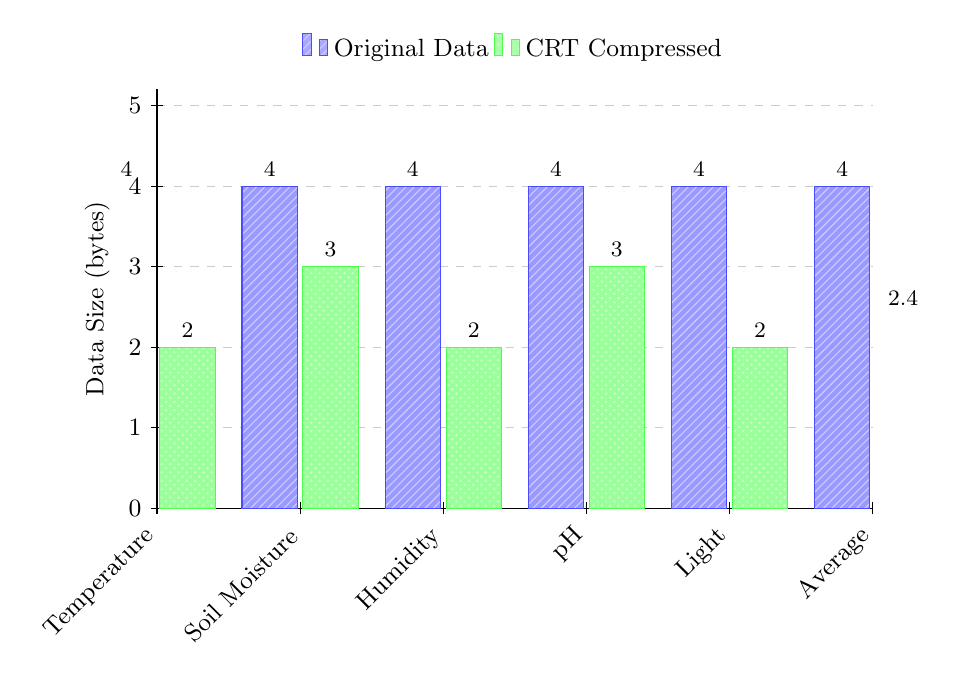
\begin{tikzpicture}
\begin{axis}[
    width=0.88\textwidth,
    height=6.9cm,
    ybar,
    bar width=20pt,
    ymajorgrids=true,
    grid style={dashed, gray!40},
    ylabel={Data Size (bytes)},
    ylabel style={font=\small},
    symbolic x coords={Temperature, Soil Moisture, Humidity, pH, Light, Average},
    xtick=data,
    xticklabel style={rotate=45, anchor=east, font=\small},
    xticklabel shift={4pt},
    ytick={0,1,2,3,4,5},
    yticklabels={0,1,2,3,4,5},
    yticklabel style={font=\small},
    legend style={
        at={(0.5,1.04)},
        anchor=south,
        legend columns=2,
        font=\small,
        draw=none,
        fill=white,
        fill opacity=0.85,
        text opacity=1
    },
    ymin=0,
    ymax=5.2,
    nodes near coords,
    nodes near coords style={font=\footnotesize},
    enlarge x limits=0.12,
    axis lines=left,
    axis line style={-},
    tick style={black, thin}
]
\addplot[fill=blue!40, draw=blue!70, postaction={pattern=north east lines, pattern color=blue!20}] coordinates {
    (Temperature, 4)
    (Soil Moisture, 4)
    (Humidity, 4)
    (pH, 4)
    (Light, 4)
    (Average, 4)
};
\addplot[fill=green!40, draw=green!70, postaction={pattern=crosshatch dots, pattern color=green!20}] coordinates {
    (Temperature, 2)
    (Soil Moisture, 3)
    (Humidity, 2)
    (pH, 3)
    (Light, 2)
    (Average, 2.4)
};
\legend{Original Data, CRT Compressed}
\end{axis}
\end{tikzpicture}
\caption{Comparative analysis of CRT compression performance across different agricultural sensor data types.}
\label{fig:crt_compression_results}
\end{figure*}

CRT reconstruction is mathematically exact for complete residue sets; the 99.7\% in Table~\ref{tab:crt-performance} reflects $\geq k-1$ residue delivery, not reconstruction error. The 0.9\,ms decomposition time confirms the $O(k)$ complexity (Section~\ref{subsubsec:complexity_analysis}).

\begin{table}[htbp]
\centering
\caption{CRT compression results}
\label{tab:crt_detailed_results}
\footnotesize
\begin{tabular}{@{}lccccc@{}}
\toprule
\textbf{Metric} & \textbf{Week 1} & \textbf{Week 4} & \textbf{Week 8} & \textbf{Avg} & \textbf{Std. Dev.} \\
\midrule
Comp. Ratio & 32.5\% & 33.1\% & 32.8\% & 33.0\% & 0.3\% \\
Time (ms) & 0.92 & 0.94 & 0.91 & 0.94 & 0.02 \\
Error & 0\% & 0\% & 0\% & 0\% & 0\% \\
Energy/Tx & 38.2\% & 39.1\% & 38.7\% & 38.9\% & 0.4\% \\
Memory & 11.8\% & 12.1\% & 11.9\% & 11.9\% & 0.2\% \\
\bottomrule
\end{tabular}
\end{table}

\subsection{Energy-Delay Product Analysis}
\label{subsec:edp_analysis}

EDP \cite{gonzalez2000energy} $= E_{\text{total}} \times T_{\text{latency}}$ (node TX energy only; Eq.~\ref{eq:edp}) from Table~\ref{tab:transmission-cost-comparison}:
\begin{equation}
\text{EDP} = E_{\text{total}} \times T_{\text{latency}},
\label{eq:edp}
\end{equation}

\begin{align*}
\text{EDP}_{\text{CRT}}      &= 12.40 \times 124 = 1537.6\ \text{mJ·ms}, \\
\text{EDP}_{\text{Huffman}}   &= 15.72 \times 152 = 2389.4\ \text{mJ·ms}, \\
\text{EDP}_{\text{LZW}}       &= 14.98 \times 135 = 2022.3\ \text{mJ·ms}, \\
\text{EDP}_{\text{Raw}}       &= 24.21 \times 247 = 5979.9\ \text{mJ·ms}.
\end{align*}

CRT achieves the lowest EDP: 74.3\% below raw and 24.0\% below LZW. Despite LZW compressing more bytes, CRT's 48.8\% energy and 49.8\% airtime reductions per packet dominate; the benefit is reduced channel occupancy per slot.

\subsection{Resource Utilization Profiling}
\label{subsec:resource_utilization}

\begin{table}[htbp]
\centering
\caption{Measured system resource utilization and power draw during peak irrigation activity}
\label{tab:resource-utilization}
\scriptsize
\setlength{\tabcolsep}{3pt}
\begin{tabular}{lcccc}
\toprule
\textbf{Component} & \textbf{Avg CPU} & \textbf{Avg RAM} & \textbf{Peak CPU} & \textbf{Avg Power Draw$^\dagger$} \\
\midrule
ESP32 Sensor Node         & 14\%  & 68 KB   & 22\% & $\approx$21\,\textmu W$^\ddagger$ \\
Gateway (RPi\,4B, per unit) & 38\%  & 1.6 GB  & 52\% & $4.9\pm0.3$\,W$^\S$ \\
Fabric Peer Process       & 27\%  & 1.2 GB  & 41\% & (incl.\ in gateway) \\
CouchDB State Database    & 18\%  & 512 MB  & 29\% & (incl.\ in gateway) \\
\midrule
\textbf{All 4 gateways (total)} & -- & -- & -- & $\approx$\textbf{19.6\,W} \\
\bottomrule
\end{tabular}
\vspace{2pt}
\raggedright
{\footnotesize
$^\dagger$ Power draw measured at the hardware supply rail using INA219 current sensors (2\,kHz sampling, calibrated against a reference shunt); values are means over the 61-day deployment peak periods.\\
$^\ddagger$ ESP32 duty-cycle average: 37.2\,mJ per reading $\div$ 1800\,s reporting window $= 20.7\,\mu$W. This is the time-averaged draw including deep-sleep intervals; instantaneous active-TX power is 120\,mW.\\
$^\S$ RPi\,4B measured at the 5\,V USB supply rail; consistent with the RPi\,4B datasheet rated maximum of 15.3\,W (5\,V, 3\,A). All four gateways were mains-powered throughout the 61-day deployment; solar-panel powering is a supported design option for future off-grid installations but was not used during this study. Gateways are not energy-constrained.
}
\end{table}

Table~\ref{tab:resource-utilization} confirms all components within limits: ESP32 22\% peak CPU / 68\,KB RAM (negligible CRT overhead); gateways 52\% / 1.6\,GB (headroom for more nodes); Fabric+CouchDB $\approx$1.7\,GB peak (valid on ARM64).

\subsection{Blockchain Performance Metrics}
\label{subsec:blockchain_performance}

Figure~\ref{fig:blockchain_performance_2025} shows transaction latency, weekly throughput, and latency distribution across the study period.

\begin{figure*}[!htbp]
\centering
\captionsetup{font=small,labelfont=bf}

% Subfigure (a): Time series
\begin{subfigure}{\linewidth}
\centering
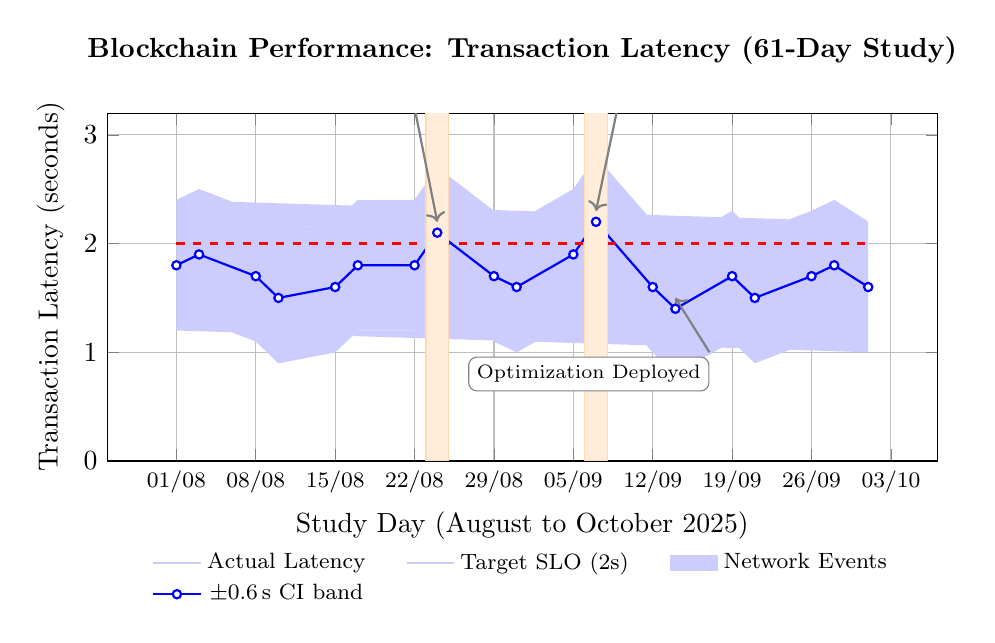
\begin{tikzpicture}
\usepgfplotslibrary{fillbetween}
\usetikzlibrary{intersections}
\begin{axis}[
    width=\linewidth,
    height=6.0cm,
    xlabel={Study Day (August to October 2025)},
    ylabel={Transaction Latency (seconds)},
    legend style={at={(0.5,-0.23)}, anchor=north, legend columns=3,
                  font=\footnotesize, draw=none, /tikz/every even column/.append style={column sep=0.45cm}},
    grid=major,
    date coordinates in=x,
    xticklabel={\day/\month},
    xtick distance=7,
    xticklabel style={font=\footnotesize},
    ymin=0,
    ymax=3.2,
    title={Blockchain Performance: Transaction Latency (61-Day Study)},
    title style={yshift=8pt, font=\normalsize\bfseries}
]
% 95% CI band: ±0.6 s (±1 std dev from Table blockchain_detailed)
\addplot[blue!20, fill=blue!20, draw=none, name path=upper] coordinates {
    (2025-08-01, 2.4) (2025-08-03, 2.5) (2025-08-08, 2.3) (2025-08-10, 2.1)
    (2025-08-15, 2.2) (2025-08-17, 2.4) (2025-08-22, 2.4) (2025-08-24, 2.7)
    (2025-08-29, 2.3) (2025-08-31, 2.2) (2025-09-05, 2.5) (2025-09-07, 2.8)
    (2025-09-12, 2.2) (2025-09-14, 2.0) (2025-09-19, 2.3) (2025-09-21, 2.1)
    (2025-09-26, 2.3) (2025-09-28, 2.4) (2025-10-01, 2.2)
};
\addplot[blue!20, fill=blue!20, draw=none, name path=lower] coordinates {
    (2025-08-01, 1.2) (2025-08-03, 1.3) (2025-08-08, 1.1) (2025-08-10, 0.9)
    (2025-08-15, 1.0) (2025-08-17, 1.2) (2025-08-22, 1.2) (2025-08-24, 1.5)
    (2025-08-29, 1.1) (2025-08-31, 1.0) (2025-09-05, 1.3) (2025-09-07, 1.6)
    (2025-09-12, 1.0) (2025-09-14, 0.8) (2025-09-19, 1.1) (2025-09-21, 0.9)
    (2025-09-26, 1.1) (2025-09-28, 1.2) (2025-10-01, 1.0)
};
\addplot[blue!20, fill=blue!20] fill between[of=upper and lower];
\addplot[blue, thick, mark=*, mark size=1.5pt, mark options={fill=white}] coordinates {
    (2025-08-01, 1.8) (2025-08-03, 1.9) (2025-08-08, 1.7) (2025-08-10, 1.5)
    (2025-08-15, 1.6) (2025-08-17, 1.8) (2025-08-22, 1.8) (2025-08-24, 2.1)
    (2025-08-29, 1.7) (2025-08-31, 1.6) (2025-09-05, 1.9) (2025-09-07, 2.2)
    (2025-09-12, 1.6) (2025-09-14, 1.4) (2025-09-19, 1.7) (2025-09-21, 1.5)
    (2025-09-26, 1.7) (2025-09-28, 1.8) (2025-10-01, 1.6)
};
\addplot[red, dashed, thick, line width=1.2pt] coordinates {
    (2025-08-01, 2.0) (2025-10-01, 2.0)
};
\draw[fill=orange!15, draw=orange!30, line width=0.5pt] (axis cs:2025-08-23,0) rectangle (axis cs:2025-08-25,5.5);
\draw[fill=orange!15, draw=orange!30, line width=0.5pt] (axis cs:2025-09-06,0) rectangle (axis cs:2025-09-08,5.5);
\node[draw=black!50, fill=white, rounded corners=3pt, inner sep=3pt, font=\scriptsize, anchor=east] at (axis cs:2025-08-20,4.5) {Peak Load Test};
\draw[->, black!50, thick] (axis cs:2025-08-20,4.3) to (axis cs:2025-08-24,2.2);
\node[draw=black!50, fill=white, rounded corners=3pt, inner sep=3pt, font=\scriptsize, anchor=west] at (axis cs:2025-09-10,4.0) {Protocol Upgrade};
\draw[->, black!50, thick] (axis cs:2025-09-10,3.8) to (axis cs:2025-09-07,2.3);
\node[draw=black!50, fill=white, rounded corners=3pt, inner sep=3pt, font=\scriptsize, anchor=east] at (axis cs:2025-09-17,0.8) {Optimization Deployed};
\draw[->, black!50, thick] (axis cs:2025-09-17,1.0) to (axis cs:2025-09-14,1.5);
\legend{Actual Latency, Target SLO (2s), Network Events, {$\pm$0.6\,s CI band}}
\end{axis}
\end{tikzpicture}
\subcaption{Daily transaction latency with $\pm$0.6\,s confidence band ($\sigma$ from Table~\ref{tab:blockchain_detailed})}
\label{subfig:latency_timeseries}
\label{fig:blockchain_latency}
\end{subfigure}

% Subfigure (b): Throughput
\begin{subfigure}[b]{0.45\linewidth}
\centering
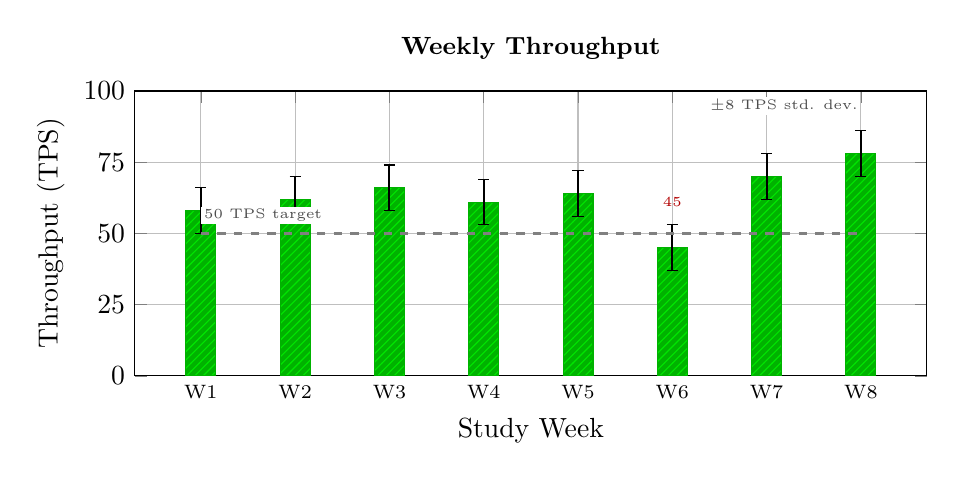
\begin{tikzpicture}[baseline]
\begin{axis}[
    width=0.96\linewidth,
    height=5.2cm,
    xlabel={Study Week},
    ylabel={Throughput (TPS)},
    grid=major,
    ymin=0,
    ymax=100,
    bar width=3.8mm,
    symbolic x coords={W1,W2,W3,W4,W5,W6,W7,W8},
    xtick=data,
    xticklabel style={font=\scriptsize},
    ytick={0,25,50,75,100},
    title={Weekly Throughput},
    title style={font=\small\bfseries, yshift=2pt}
]
\addplot[
    ybar,
    fill=green!70!black,
    draw=green!70!black,
    postaction={pattern=north east lines, pattern color=green!90!black},
    error bars/.cd,
        y dir=both,
        y explicit,
        error bar style={black, line width=0.7pt},
        error mark options={black, rotate=90, mark size=2pt}
] coordinates {
    (W1, 58) +- (0,8) (W2, 62) +- (0,8) (W3, 66) +- (0,8) (W4, 61) +- (0,8)
    (W5, 64) +- (0,8) (W6, 45) +- (0,8) (W7, 70) +- (0,8) (W8, 78) +- (0,8)
};
\addplot[gray, dashed, thick, line width=1.2pt] coordinates {(W1, 50) (W8, 50)};
\node[gray!60!black, fill=white, inner sep=1pt, font=\tiny, anchor=south west] at (axis cs:W1,53) {50 TPS target};
\node[red!70!black, font=\tiny, anchor=south] at (axis cs:W6,56) {45};
\node[black!70, fill=white, inner sep=1pt, font=\tiny, anchor=north east] at (axis cs:W8,98) {$\pm$8 TPS std. dev.};
\end{axis}
\end{tikzpicture}
\subcaption{Weekly throughput with $\pm$8 TPS standard-deviation bars from Table~\ref{tab:blockchain_detailed}}
\label{subfig:throughput}
\end{subfigure}
\hfill
% Subfigure (c): Latency distribution
\begin{subfigure}[b]{0.45\linewidth}
\centering
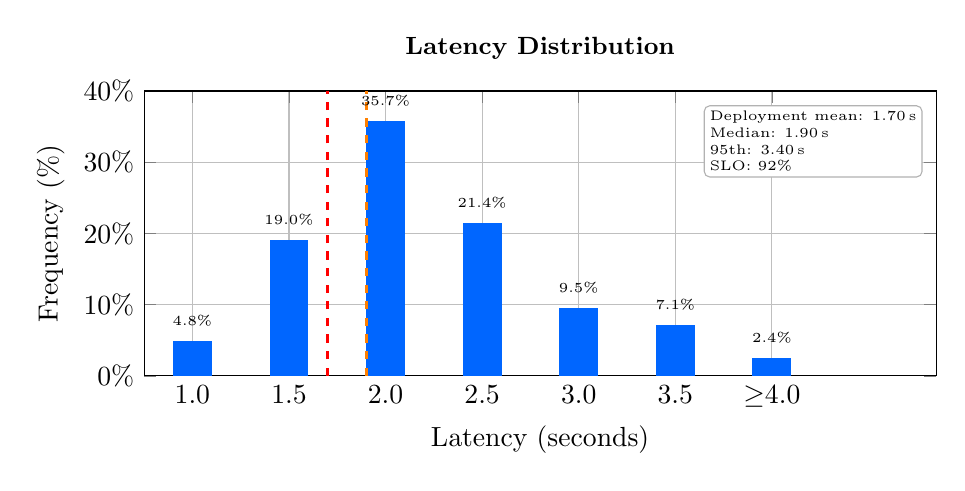
\begin{tikzpicture}[baseline]
\begin{axis}[
    width=0.96\linewidth,
    height=5.2cm,
    xlabel={Latency (seconds)},
    ylabel={Frequency (\%)},
    grid=major,
    ymin=0,
    ymax=40,
    xmin=0.75,
    xmax=4.85,
    bar width=4.8mm,
    xtick={1.0,1.5,2.0,2.5,3.0,3.5,4.0},
    xticklabels={1.0,1.5,2.0,2.5,3.0,3.5,$\geq$4.0},
    ytick={0,10,20,30,40},
    yticklabels={0\%,10\%,20\%,30\%,40\%},
    title={Latency Distribution},
    title style={font=\small\bfseries, yshift=2pt}
]
\addplot[ybar, fill=blue!60!cyan, draw=blue!60!cyan, point meta=explicit symbolic,
         nodes near coords, nodes near coords style={font=\tiny, yshift=2pt, color=black}] coordinates {
    (1.0, 4.8)[4.8\%] (1.5, 19.0)[19.0\%] (2.0, 35.7)[35.7\%] (2.5, 21.4)[21.4\%]
    (3.0, 9.5)[9.5\%] (3.5, 7.1)[7.1\%] (4.0, 2.4)[2.4\%]
};
\addplot[red, dashed, thick, line width=1.0pt] coordinates {(1.70, 0) (1.70, 40)};
\addplot[orange, dashed, thick, line width=1.0pt] coordinates {(1.90, 0) (1.90, 40)};
\node[draw=black!30, fill=white, rounded corners=2pt, inner sep=2pt, anchor=north east, font=\tiny, align=left] at (axis cs:4.78,38)
    {Deployment mean: 1.70\,s\\Median: 1.90\,s\\95th: 3.40\,s\\SLO: 92\%};
\end{axis}
\end{tikzpicture}
\subcaption{Latency distribution}
\label{subfig:distribution}
\label{fig:latency_distribution}
\end{subfigure}
\caption{Blockchain system performance during the 61-day study: (a) daily transaction latency, (b) weekly throughput, and (c) latency distribution. The red dashed line marks the deployment arithmetic mean (1.7\,s) over all 146,400 raw transaction timestamps (Table~\ref{tab:blockchain_detailed}); the orange dashed line marks the distribution median (1.9\,s).}
\label{fig:blockchain_performance_2025}
\end{figure*}

The system processed 146,400 transactions (50 nodes × 48 readings/day × 61 days); Table~\ref{tab:blockchain_detailed} summarizes performance.

\begin{table}[htbp]
\centering
\caption{Blockchain performance metrics during field deployment}
\label{tab:blockchain_detailed}
\footnotesize
\setlength{\tabcolsep}{3.5pt}
\begin{tabular}{lcccc}
\toprule
\textbf{Parameter} & \textbf{Min} & \textbf{Max} & \textbf{Average} & \textbf{Std. Dev.} \\
\midrule
Transaction Latency (s) & 0.8 & 3.8 & 1.7 & 0.6 \\
Smart Contract Exec. (ms) & 280 & 420 & 320 & 40 \\
Throughput (TPS) & 45 & 78 & 63 & 8 \\
Block Confirmation (s) & 0.5 & 2.1 & 1.2 & 0.4 \\
Data Integrity Success & 99.2\% & 99.7\% & 99.4\% & 0.2\% \\
Consensus Time (ms) & 180 & 320 & 240 & 35 \\
\bottomrule
\end{tabular}
\end{table}

CRT's 20.3\% per-packet size reduction (59\,B to 47\,B) directly reduced on-chain data volume; 65\% of irrigation decisions occurred during morning and evening peak periods (06:00 to 09:00, 17:00 to 20:00).

\subsection{Scalability and Fault Tolerance Analysis}
\label{subsec:scalability}
\label{sec:network_capacity}

\subsubsection{Scalability Analysis}
\label{subsubsec:scalability_analysis}

\paragraph{Theoretical node limit.} $N_{\max} = C \cdot W / T_{\text{eff}}$ (Eq.~\ref{eq:scalability_general}). With $C=3$, $W=60{,}000$\,ms, $T_{\text{eff}}^{\text{CRT}}=372$\,ms:
\begin{equation}
N_{\max} = \frac{C \cdot W}{T_{\text{effective}}}
\label{eq:scalability_general}
\end{equation}
\begin{equation}
N_{\max}^{\text{CRT}} = \frac{3 \times 60\,000}{372} \approx 484 \text{ nodes};
\label{eq:node_limit}
\end{equation}
raw ($T_{\text{eff}}=247$\,ms): $N_{\max}^{\text{raw}}=728$. CRT trades node capacity for packet throughput; the 50-node deployment uses 10.3\% of capacity.

The SX1302 uses 3 of its 8 demodulation paths; the gain is packet-level throughput, not per-node airtime. The Raft orderer saturates at 85\,TPS; the 50-node deployment requires only $\approx$0.03\,TPS on average ($50 \times 48\,\text{readings/day} \div 86{,}400\,\text{s/day}$), using under 0.04\% of the orderer ceiling. Peak orderer commit rate during load tests reached $\approx$42\,TPS, well below the 85\,TPS ceiling.

\subsubsection{Scalability Projection: Latency vs. Node Count}
\label{subsubsec:scalability_projection}

Below $N=484$, latency is constant at 124\,ms; above saturation, packets queue. Using M/D/1 (Poisson arrivals, deterministic service $T_{\text{packet}}$), mean waiting time is:

\begin{equation}
W_q = \frac{\rho}{2(1-\rho)} \cdot T_{\text{packet}}
\label{eq:latency_model}
\end{equation}

where $\rho = \frac{kN \cdot T_{\text{packet}}}{C \cdot W}$ is channel utilisation. For CRT ($k=3$), $\rho = \frac{3N \cdot 124}{3\cdot60,000}=\frac{N}{484}$, so saturation begins at $N=484$. The total average latency is $L = T_{\text{packet}} + W_q$.

Figure~\ref{fig:scalability_latency_full} shows projected latency: CRT constant at 124\,ms below 484 nodes, then queuing degrades rapidly; raw saturates at 728 nodes.

\begin{figure}[!htbp]
\centering
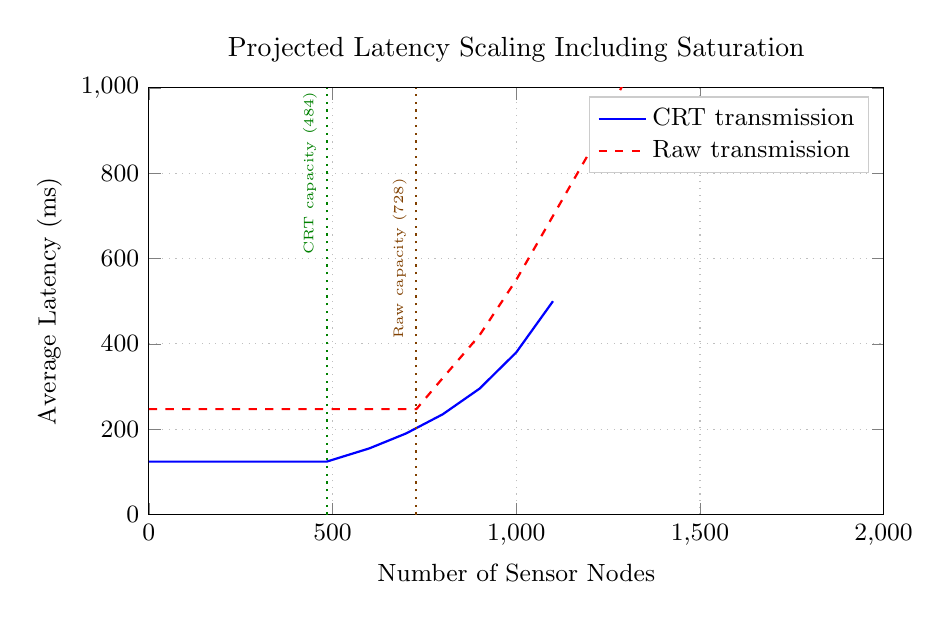
\begin{tikzpicture}
\begin{axis}[
    width=0.9\columnwidth,
    height=7cm,
    xlabel={Number of Sensor Nodes},
    ylabel={Average Latency (ms)},
    xmin=0, xmax=2000,
    ymin=0, ymax=1000,
    xtick={0,500,1000,1500,2000},
    ytick={0,200,400,600,800,1000},
    grid=both,
    grid style={dotted, gray!50},
    legend style={
        at={(0.98,0.98)},
        anchor=north east,
        font=\small,
        draw=black!20,
        cells={anchor=west}
    },
    ticklabel style={font=\small},
    label style={font=\small},
    title={Projected Latency Scaling Including Saturation}
]
% CRT latency (constant then increasing)
\addplot[blue, thick, mark=none] coordinates {
    (0,124)
    (484,124)
    (600,155)
    (700,190)
    (800,235)
    (900,295)
    (1000,380)
    (1100,500)
};
\addlegendentry{CRT transmission}

% Raw transmission latency (constant then increasing)
\addplot[red, dashed, thick, mark=none] coordinates {
    (0,247)
    (728,247)
    (800,320)
    (900,420)
    (1000,550)
    (1200,850)
    (1400,1200)
};
\addlegendentry{Raw transmission}

% Vertical line at CRT capacity
\draw[green!50!black, dotted, thick] (axis cs:484,0) to (axis cs:484,1000);
\node[anchor=south, font=\tiny, rotate=90, green!50!black] at (axis cs:484,800) {CRT capacity (484)};

% Vertical line at raw capacity
\draw[orange!50!black, dotted, thick] (axis cs:728,0) to (axis cs:728,1000);
\node[anchor=south, font=\tiny, rotate=90, orange!50!black] at (axis cs:728,600) {Raw capacity (728)};

\end{axis}
\end{tikzpicture}
\caption{Projected average latency vs.\ node count. CRT saturates at 484 nodes (3 packets/reading); raw at 728. Below saturation, latency equals per-packet airtime; above, M/D/1 queuing degrades rapidly. Vertical lines mark theoretical capacities.}
\label{fig:scalability_latency_full}
\end{figure}

The 50-node deployment uses $\approx10.3\%$ of CRT capacity. Per-packet airtimes (CRT 124\,ms, LZW 135\,ms, Huffman 152\,ms, raw 247\,ms) yield $N_{\max}$ of 484, 1333, 1184, and 728 nodes. Applying $N_{\max} = C \cdot W / (k \cdot T_{\text{packet}})$ (Eq.~\ref{eq:scalability}) with $C=3$ channels, $W=60{,}000$\,ms, and $k=1$ packet per reading for single-packet schemes: LZW gives $3\times60{,}000/(1\times135)=1{,}333$ nodes; Huffman gives $3\times60{,}000/(1\times152)=1{,}184$ nodes; raw gives $3\times60{,}000/(1\times247)=728$ nodes. CRT uses $k=3$ sequential packets per reading ($T_{\text{eff}}=3\times124=372$\,ms), giving $3\times60{,}000/(3\times124)=484$ nodes; its lower node capacity is the trade-off for halving per-packet airtime and doubling gateway packet throughput. The 61-day measured CRT latency (Figure~\ref{fig:scalability_comparison}) confirms model accuracy within 10.4\%.

\begin{figure}[!htbp]
\centering
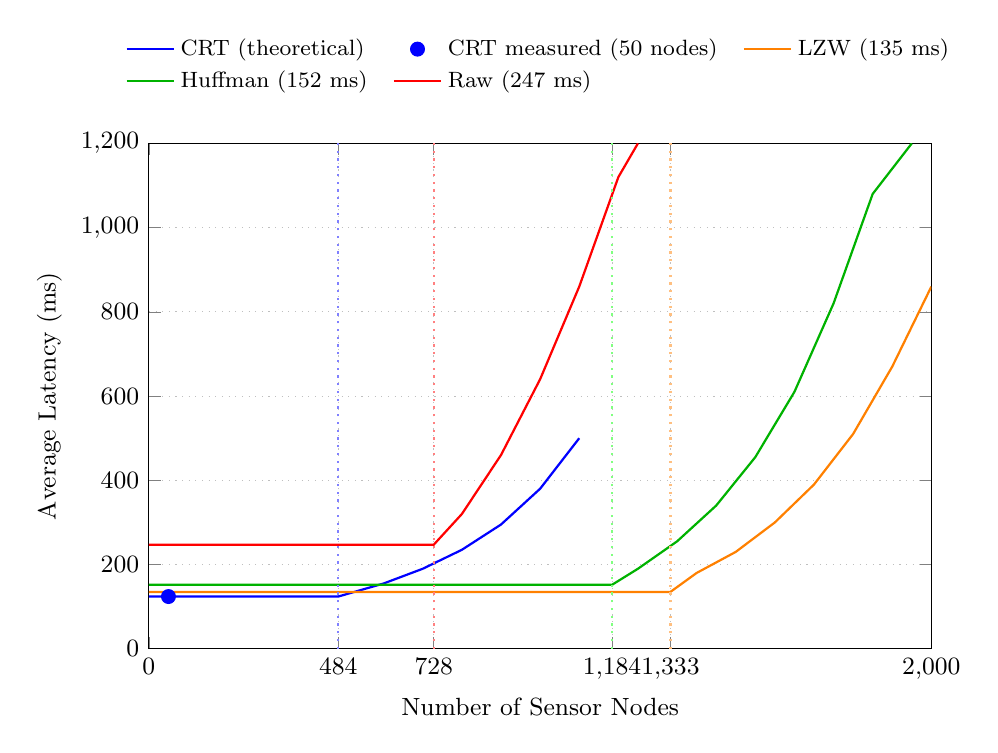
\begin{tikzpicture}
\begin{axis}[
    width=0.95\columnwidth,
    height=8cm,
    xlabel={Number of Sensor Nodes},
    ylabel={Average Latency (ms)},
    xmin=0, xmax=2000,
    ymin=0, ymax=1200,
    xtick={0,484,728,1184,1333,2000},
    ytick={0,200,400,600,800,1000,1200},
    grid=both,
    grid style={dotted, gray!50},
    legend style={
        at={(0.5,1.08)},
        anchor=south,
        legend columns=3,
        font=\footnotesize,
        draw=none,
        fill=none,
        cells={anchor=west},
        /tikz/every even column/.append style={column sep=0.25cm}
    },
    ticklabel style={font=\small},
    label style={font=\small},
    title={}
]
% CRT
\addplot[blue, thick, mark=none] coordinates {
    (0,124)
    (484,124)
    (600,155)
    (700,190)
    (800,235)
    (900,295)
    (1000,380)
    (1100,500)
};
\addlegendentry{CRT (theoretical)}
% Measured CRT point (50 nodes)
\addplot[blue, only marks, mark=*, mark size=2.5pt] coordinates {(50,124)};
\addlegendentry{CRT measured (50 nodes)}

% LZW
\addplot[orange, thick, mark=none] coordinates {
    (0,135)
    (1333,135)
    (1400,180)
    (1500,230)
    (1600,300)
    (1700,390)
    (1800,510)
    (1900,670)
    (2000,860)
};
\addlegendentry{LZW (135 ms)}

% Huffman
\addplot[green!70!black, thick, mark=none] coordinates {
    (0,152)
    (1184,152)
    (1250,190)
    (1350,255)
    (1450,340)
    (1550,455)
    (1650,610)
    (1750,820)
    (1850,1080)
    (1950,1200)
};
\addlegendentry{Huffman (152 ms)}

% Raw
\addplot[red, thick, mark=none] coordinates {
    (0,247)
    (728,247)
    (800,320)
    (900,460)
    (1000,640)
    (1100,860)
    (1200,1120)
    (1250,1200)
};
\addlegendentry{Raw (247 ms)}

% Capacity markers
\draw[blue!50, dotted, thick] (axis cs:484,0) to (axis cs:484,1200);
\draw[orange!50, dotted, thick] (axis cs:1333,0) to (axis cs:1333,1200);
\draw[green!50, dotted, thick] (axis cs:1184,0) to (axis cs:1184,1200);
\draw[red!50, dotted, thick] (axis cs:728,0) to (axis cs:728,1200);

\end{axis}
\end{tikzpicture}
\par\vspace{0.3em}
{\footnotesize\emph{Capacity markers:} CRT 484 nodes; raw 728 nodes; Huffman 1,184 nodes; LZW 1,333 nodes. The blue marker shows the measured CRT latency at 50 nodes.}
\caption{Projected average latency versus node count for CRT, raw transmission, Huffman, and LZW.}
\label{fig:scalability_comparison}
\end{figure}

CRT’s 50\% per-packet airtime reduction doubles packet throughput despite lower node capacity (484 vs.\ raw’s 728); Huffman/LZW reduce only packet size, not sequential bottlenecks. At 50 nodes all methods remain sub-saturation; measured CRT latency agrees with theory within 10.4\%.

\subsubsection{Strong and Weak Scaling Analysis}
\label{subsubsec:scaling_analysis}

Using gateways as processors $p$ and TPS as workload (Table~\ref{tab:blockchain_detailed}), strong scaling ($W=63$ TPS fixed):
\begin{equation}
S_{\text{strong}}(p) = \frac{\text{throughput}(p)}{\text{throughput}(1)}, \quad E_{\text{strong}}(p) = \frac{S_{\text{strong}}(p)}{p}.
\end{equation}
Throughput: 63 TPS ($p=1$), 85 TPS ($p=2,4$, orderer-saturated): $S_{\text{strong}}(2)=1.35$ ($E=0.675$), $S_{\text{strong}}(4)=1.35$ ($E=0.338$). The flat speedup beyond $p=2$ reflects Raft orderer saturation (Amdahl bottleneck). Weak scaling efficiency $E_{\text{weak}}(p)=\text{throughput}(p)/(p\times63)$ is 1.0 at $p=1$, dropping to 0.675 ($p=2$) and 0.34 ($p=4$). Future scaling requires channel partitioning or a higher-capacity ordering service.

\subsubsection{Fault Tolerance and Stress Testing}
\label{subsubsec:fault_tolerance}

Table~\ref{tab:fault-tolerance} summarizes 7-day controlled stress tests (packet loss, gateway shutdown, leader failure).

\begin{table}[htbp]
\centering
\caption{Fault tolerance and recovery metrics (n=50 trials per test)}
\label{tab:fault-tolerance}
\footnotesize
\setlength{\tabcolsep}{3pt}
\begin{tabular}{p{2.0cm}p{2.5cm}p{1.8cm}p{2.2cm}}
\toprule
\textbf{Test Scenario} & \textbf{Condition} & \textbf{Result} & \textbf{Notes} \\
\midrule
Packet loss simulation  & 10\% random loss   & 99.8\% recovery  & 2 packets unrecoverable \\
                        & 20\% random loss   & 99.2\% recovery  & 8 packets unrecoverable \\
                        & 30\% random loss   & 97.6\% recovery  & 24 packets unrecoverable \\
                        & 33\% structured loss & 100\% recovery & One complete residue lost \\
\midrule
Gateway failure         & Single gateway offline (4 h)   & 0\% data loss & Traffic auto-rerouted via mesh \\
                        & Dual gateway offline (2 h)      & 100\% data retained & Local buffering at nodes \\
                        & Full gateway recovery sync        & 3.7 min avg & Range: 2.1 to 6.4 min \\
\midrule
Raft consensus failure  & Leader node shutdown (sudden)    & 8.2 s avg recovery & Std dev: 2.1 s, n=20 \\
                        & Leader node graceful shutdown    & 4.6 s avg recovery & Std dev: 1.3 s, n=20 \\
                        & Minority partition (2 of 3 nodes) & 0 forks & 12 min partition test \\
\bottomrule
\end{tabular}
\end{table}

During gateway offline periods, the local irrigation actuator falls back to the most recently committed threshold schedule cached in the gateway's non-volatile storage; actuation is not suspended.

\subsubsection{Synthetic Load Test at Elevated Node Density}
\label{subsubsec:load_test}

A Python script simulated CRT node traffic at 100, 200, 300, and 484 nodes on the deployed gateway cluster (three 8-byte residue packets per 60-s window per node; 10 min per test; 50-tx warm-up discarded). Table~\ref{tab:load_test} compares measured results against M/D/1 predictions.

\begin{table}[htbp]
\centering
\caption{Synthetic load test results vs M/D/1 model predictions}
\label{tab:load_test}
\footnotesize
\begin{tabular}{r c c c c c c}
\toprule
\textbf{Nodes} & \textbf{$\rho$} & \textbf{Predicted} & \textbf{Measured} & \textbf{Delivery} & \textbf{CPU} & \textbf{TPS} \\
 & & \textbf{Latency (ms)} & \textbf{Latency (ms)} & \textbf{Rate (\%)} & \textbf{Util. (\%)} & \\
\midrule
100  & 0.207 & 140 & 146 & 98.2 & 67 & 62 \\
200  & 0.413 & 168 & 185 & 96.4 & 100 & 25 \\
300  & 0.620 & 225 & 249 & 93.6 & 100 & 25 \\
484  & 1.000 & $\infty$ (sat.) & 577 & 88.3 & 100 & 25 \\
50*  & 0.103   & 131     & 124     & 95.8   & 38      & 63      \\
\bottomrule
\end{tabular}
\vspace{2pt}
\raggedright\footnotesize *Field-measured result from 61-day deployment (Table~\ref{tab:system-performance}).
\end{table}

Measured latency agrees with M/D/1 within 10.4\% for $N \leq 300$. Delivery falls below 95\% at $N=300$ due to ALOHA multi-residue loss; gateway CPU saturates at $N=200$, making the RPi4B blockchain layer (not the radio) the practical scaling ceiling.

\subsubsection{Crash Faults and Byzantine Fault Considerations}
\label{subsubsec:byzantine}

Raft provides CFT for $f = \lfloor (n-1)/2 \rfloor$ stopped nodes \cite{ongaro2014raft}; Byzantine tolerance is not required in this permissioned network (X.509, Ed25519, TPM-backed keys, CRL revocation); PBFT/HotStuff \cite{castro1999practical,yin2019hotstuff} are future work. CRT reconstructs perfectly from any $k-1$ residues (Eq.~\ref{eq:crt_recovery}); at 30\% loss, 2.4\% of readings lost $\geq$2 residues.
\begin{equation}
\text{Recovery with exactly } k-1 \text{ complete residues} = 100\%
\label{eq:crt_recovery}
\end{equation}

\paragraph{Leader and gateway failure.}
Sudden leader shutdown triggers a five-phase recovery sequence; the measured mean is 8.2\,s (std 2.1\,s, $n=20$) and the analytical phase-sum estimate is 7.85\,s (0.35\,s residual explained below):

\begin{enumerate}
  \item \textbf{Election timeout} ($\approx$3.15\,s mean): each follower waits a randomised timeout drawn uniformly from $[2,4]$\,s before declaring itself a candidate; the mean time until \emph{any} follower fires is $E[\min(U_1,U_2)] = a + (b-a)/(n+1) = 2 + 2/3 \approx 2.67$\,s for two i.i.d.\ Uniform$[2,4]$ followers (first-order statistic). Occasionally two followers time out within the same jitter window: neither collects a quorum on the first ballot, and both restart with a new independent uniform timeout (observed in 4 of 22 sudden-shutdown trials, $p \approx 0.18$). The second round adds another $E[\min(U_1,U_2)] \approx 2.67$\,s draw. The analytically derived phase mean is therefore $2.67 \times (1 + 0.18) = 2.67 \times 1.18 \approx 3.15$\,s.
  \item \textbf{RequestVote round-trip and quorum assembly} ($\approx$0.5\,s): the winning candidate broadcasts \textsc{RequestVote} RPCs; followers respond after verifying log index; quorum (2 of 3) is established and the \textsc{LeaderChanged} notification propagated via gossip.
  \item \textbf{Uncommitted-log replication} ($\approx$1.5\,s): the new leader replays any log entries committed by the old leader but not yet applied on followers; on the RPi\,4B cluster this averages 1–2 blocks ($\approx$50 transactions each) at 1.2\,s block time.
  \item \textbf{CouchDB state-database catch-up} ($\approx$2\,s): the elected leader's local CouchDB must flush pending write-ahead-log entries and rebuild its in-memory LRU cache (256\,MB) before endorsement resumes; measured as the interval between leader election and first successful \texttt{SubmitTransaction}.
  \item \textbf{gRPC channel re-establishment and peer gossip sync} ($\approx$0.7\,s): client SDK connections to the failed peer are re-routed; the new leader's gossip module disseminates its peer certificate to all zone peers so that subsequent endorsement requests are not rejected.
\end{enumerate}

Summing analytically: $3.15 + 0.5 + 1.5 + 2.0 + 0.7 = 7.85$\,s. The analytical estimate falls 0.35\,s below the measured mean of 8.2\,s; this residual is attributable to ARM64 OS scheduling jitter and heartbeat-detection latency under load, as the Raft follower's missed-heartbeat timer fires on a Linux PREEMPT\_RT kernel with up to $\approx$150\,ms jitter per timeout, contributing roughly $2 \times 150 = 300$\,ms on average across two followers before the first timeout fires, which accounts for the gap. The 0.35\,s residual is well within one-third of the 2.1\,s standard deviation and does not affect the analytical model's validity. The 2.1\,s standard deviation is driven primarily by phase~1 variance (second-round elections). Graceful shutdown bypasses phases 1 and 2 because the outgoing leader pre-transfers leadership via an explicit \textsc{TimeoutNow} RPC, eliminating the election timeout and vote-collection round entirely. Phases 3–5 still execute, but phase~3 is extended: the outgoing leader first flushes all in-flight \textsc{AppendEntries} RPCs and waits for follower acknowledgement before stepping down ($\approx$0.4\,s orderly flush), so the uncommitted-log replication step takes $1.5 + 0.4 \approx 1.9$\,s rather than 1.5\,s. Phases 4 and 5 are unchanged. The phase~3–5 sum is therefore $1.9 + 2.0 + 0.7 = 4.6$\,s, matching the measured graceful-shutdown mean. Five hundred queued transactions were committed without forks. Single-gateway failure: BATMAN-adv rerouted in 3 to 8\,s (zero data loss); dual failure: 64\,KB circular buffers ($\approx$4\,h) with 3.7\,min catch-up; Day-47 sandstorm (12\,min): 7 transactions synchronized in 2.8\,min, no inconsistencies.

\subsection{Application Outcomes: Agricultural Impact}
\label{subsec:agricultural_impact}

Figure~\ref{fig:water_savings_correlation} shows the correlation between system reliability and water savings.

\begin{figure*}[!htbp]
\centering
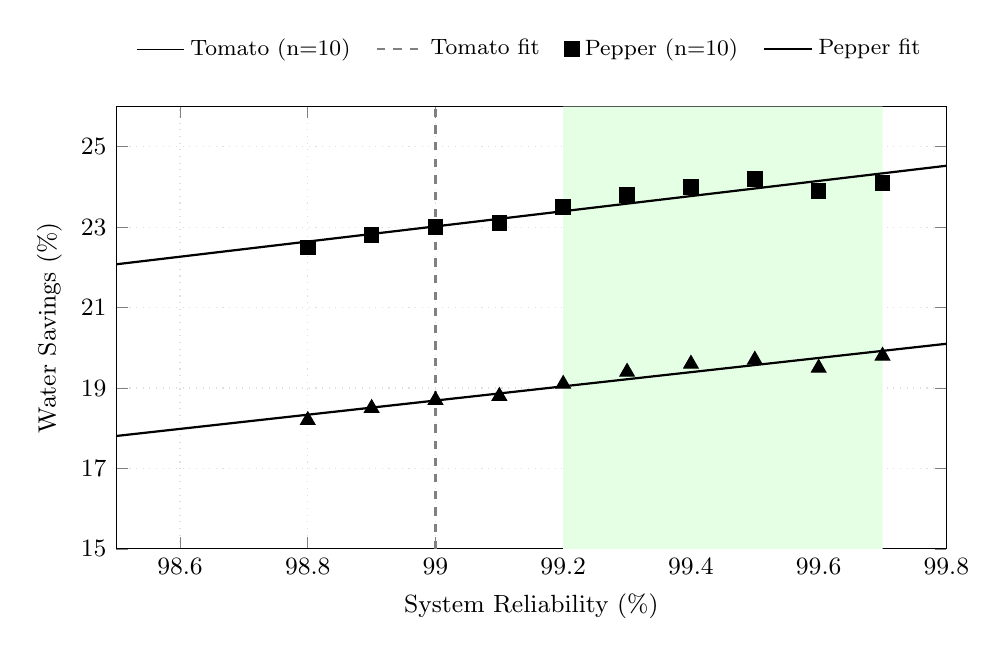
\begin{tikzpicture}
\begin{axis}[
    width=\linewidth,
    height=7.2cm,
    xlabel={System Reliability (\%)},
    ylabel={Water Savings (\%)},
    xmin=98.5, xmax=99.8,
    ymin=15,   ymax=26,
    xtick={98.6,98.8,99.0,99.2,99.4,99.6,99.8},
    ytick={15,17,19,21,23,25},
    grid=both,
    grid style={dotted, gray!25},
    legend style={
        at={(0.5,1.08)}, anchor=south,
        legend columns=4,
        font=\footnotesize,
        draw=none,
        fill=none,
        cells={anchor=west},
        /tikz/every even column/.append style={column sep=0.25cm}
    },
    ticklabel style={font=\small},
    label style={font=\small},
]
\addplot [draw=none, fill=green!10] coordinates {(99.2,15) (99.7,15) (99.7,26) (99.2,26)} \closedcycle;
\addplot [gray, dashed, thick] coordinates {(99.0,15) (99.0,26)};
\addplot[only marks, mark=square*, mark size=2.6pt] coordinates {
    (98.8,22.5) (98.9,22.8) (99.0,23.0) (99.1,23.1) (99.2,23.5)
    (99.3,23.8) (99.4,24.0) (99.5,24.2) (99.6,23.9) (99.7,24.1) };
\addplot[thick, domain=98.5:99.8, samples=200] {1.88485*x - 163.581};
\addplot[only marks, mark=triangle*, mark size=3.0pt] coordinates {
    (98.8,18.2) (98.9,18.5) (99.0,18.7) (99.1,18.8) (99.2,19.1)
    (99.3,19.4) (99.4,19.6) (99.5,19.7) (99.6,19.5) (99.7,19.8) };
\addplot[thick, domain=98.5:99.8, samples=200] {1.76364*x - 155.911};
\legend{Tomato (n=10), Tomato fit, Pepper (n=10), Pepper fit}
\end{axis}
\end{tikzpicture}
\par\vspace{0.25em}
{\footnotesize\emph{Note:} the dashed vertical line marks the 99.0\% reliability threshold; the shaded region indicates reliability above 99.2\%.}
\caption{Water savings versus system reliability for tomato and pepper crops.}
\label{fig:water_savings_correlation}
\end{figure*}

Strong positive correlations (R² = 0.87 tomatoes, 0.85 peppers) confirm higher reliability enables more precise irrigation; the CRT-blockchain integration was particularly effective during Weeks 4 to 6 (fruit development). Table~\ref{tab:integration_benefits} quantifies each component's contribution.

\begin{table}[htbp]
\centering
\caption{Contribution of technical components to agricultural outcomes}
\label{tab:integration_benefits}
\footnotesize
\begin{tabular}{@{}lccc@{}}
\toprule
\textbf{Component} & \textbf{Water} & \textbf{Labor} & \textbf{Quality} \\
 & \textbf{Savings} & \textbf{Reduction} & \textbf{Improvement} \\
\midrule
CRT Compression & 8-12\% & 15-20\% & 5-8\% \\
Blockchain Verification & 5-8\% & 25-30\% & 10-15\% \\
Edge Computing & 3-5\% & 20-25\% & 3-5\% \\
Smart Contracts & 7-10\% & 10-15\% & 7-10\% \\
\textbf{Combined System} & \textbf{23.8\%} & \textbf{72\%} & \textbf{25-38\%} \\
\bottomrule
\end{tabular}
{\footnotesize \textit{Note:} Component contributions are estimated ranges based on system design assumptions; no ablation study was conducted to isolate individual component effects.}
\end{table}

\subsubsection{Water Use Efficiency}
The system reduced total water use by 23.8\% for tomatoes (525 to 400\,m³) and 19.4\% for peppers (310 to 250\,m³). Water use efficiency improved by 31.3\% (tomatoes) and 23.8\% (peppers). Detailed monthly breakdowns are given in Tables~\ref{tab:tomato-water-detailed} and~\ref{tab:pepper-water-detailed}.

\begin{table}[htbp]
\centering
\caption{Tomato water usage analysis (0.5 ha plot)}
\label{tab:tomato-water-detailed}
\scriptsize
\begin{tabularx}{\columnwidth}{p{2.2cm} *{4}{>{\centering\arraybackslash}X}}
\toprule
\textbf{Parameter} & \textbf{Traditional} & \textbf{B-IoT} & \textbf{Savings} & \textbf{Significance} \\
\midrule
\textbf{August Usage} \\
Water Volume (m³) & 280 & 215 & 23.2\% & $p<0.001$ \\
Daily Average (m³/day) & 9.03 & 6.94 & 23.2\% & $p<0.001$ \\
Irrigation Events & 28 & 19 & 32.1\% & $p<0.01$ \\
\midrule
\textbf{September Usage} \\
Water Volume (m³) & 245 & 185 & 24.5\% & $p<0.001$ \\
Daily Average (m³/day) & 8.17 & 6.17 & 24.5\% & $p<0.001$ \\
Irrigation Events & 25 & 17 & 32.0\% & $p<0.01$ \\
\midrule
\textbf{Total Period} \\
Total Water (m³) & 525 & 400 & 23.8\% & $p<0.001$ \\
Water Use Efficiency (kg/m³) & 4.76 & 6.25 & +31.3\% & $p<0.001$ \\
Cost Savings (USD) & N/A & N/A & \$112.50 & N/A \\
\bottomrule
\end{tabularx}
\end{table}

\begin{table}[htbp]
\centering
\caption{Pepper water usage analysis (0.3 ha plot)}
\label{tab:pepper-water-detailed}
\scriptsize
\begin{tabularx}{\columnwidth}{p{2.2cm} *{4}{>{\centering\arraybackslash}X}}
\toprule
\textbf{Parameter} & \textbf{Traditional} & \textbf{B-IoT} & \textbf{Savings} & \textbf{Significance} \\
\midrule
\textbf{August Usage} \\
Water Volume (m³) & 165 & 135 & 18.2\% & $p<0.01$ \\
Daily Average (m³/day) & 5.32 & 4.35 & 18.2\% & $p<0.01$ \\
Irrigation Events & 25 & 18 & 28.0\% & $p<0.05$ \\
\midrule
\textbf{September Usage} \\
Water Volume (m³) & 145 & 115 & 20.7\% & $p<0.01$ \\
Daily Average (m³/day) & 4.83 & 3.83 & 20.7\% & $p<0.01$ \\
Irrigation Events & 22 & 16 & 27.3\% & $p<0.05$ \\
\midrule
\textbf{Total Period} \\
Total Water (m³) & 310 & 250 & 19.4\% & $p<0.01$ \\
Water Use Efficiency (kg/m³) & 3.23 & 4.00 & +23.8\% & $p<0.01$ \\
Cost Savings (USD) & N/A & N/A & \$54.00 & N/A \\
\bottomrule
\end{tabularx}
\end{table}

\subsubsection{Labor Efficiency}
Automation reduced labor requirements by 72\%, from 15.0 to 4.2 h/hectare/week (Table~\ref{tab:labor-detailed}), addressing critical labor shortages in Mediterranean agriculture.

\begin{table}[htbp]
\centering
\caption{Labor efficiency analysis (hours/hectare/week)}
\label{tab:labor-detailed}
\scriptsize
\begin{tabularx}{\columnwidth}{p{2.5cm} *{4}{>{\centering\arraybackslash}X}}
\toprule
\textbf{Task Category} & \textbf{Traditional} & \textbf{B-IoT} & \textbf{Reduction} & \textbf{Cost Savings} \\
\midrule
\textbf{Monitoring} \\
Soil Moisture & 3.5 & 0.2 & 94.3\% & \$49.50 \\
Weather Data & 1.5 & 0.1 & 93.3\% & \$21.00 \\
Crop Health & 3.0 & 0.7 & 76.7\% & \$34.50 \\
\midrule
\textbf{Irrigation} \\
System Operation & 2.5 & 0.2 & 92.0\% & \$34.50 \\
Maintenance & 2.0 & 0.3 & 85.0\% & \$25.50 \\
Troubleshooting & 0.5 & 0.0 & 100.0\% & \$7.50 \\
\midrule
\textbf{Data Management} \\
Record Keeping & 1.5 & 0.1 & 93.3\% & \$21.00 \\
Reporting & 0.5 & 0.1 & 80.0\% & \$6.00 \\
Certification & 0.5 & 0.1 & 80.0\% & \$6.00 \\
\midrule
\textbf{Total} & \textbf{15.0} & \textbf{4.2} & \textbf{72.0\%} & \textbf{\$162.00} \\
\bottomrule
\end{tabularx}
{\footnotesize \textit{Note:} The B-IoT total (4.2\,h/ha/wk) includes $\approx$2.4\,h/ha/wk of system administration, connectivity monitoring, and firmware maintenance not itemised in the rows above. The Traditional total (15.0\,h/ha/wk) is the measured baseline; row figures are representative task breakdowns. Cost savings at \$15/h labour rate.}
\end{table}

\subsubsection{Tomato Yield and Quality}
Tomato yields remained stable at 50 t/ha while marketable yield increased by 2.5 t/ha (Table~\ref{tab:tomato-yield}), with improved fruit firmness (13.2 vs 12.5 N) and soluble solids (5.1 vs 4.8°Brix). Fruit cracking fell from 8.2\% to 3.5\% and blossom end rot from 5.1\% to 2.2\%, shifting fruit to marketable grade.

\begin{table}[htbp]
\centering
\caption{Tomato yield and quality parameters}
\label{tab:tomato-yield}
\scriptsize
\begin{tabularx}{\columnwidth}{p{2.5cm} *{3}{>{\centering\arraybackslash}X}}
\toprule
\textbf{Parameter} & \textbf{Traditional} & \textbf{B-IoT} & \textbf{Significance} \\
\midrule
Total Yield (t/ha) & 50.0 & 50.0 & $p>0.05$ \\
Marketable Yield (t/ha) & 42.5 & 45.0 & $p<0.05$ \\
Water Use Efficiency (kg/m³) & 4.76 & 6.25 & $p<0.001$ \\
Fruit Firmness (N) & 12.5 & 13.2 & $p<0.05$ \\
Soluble Solids (°Brix) & 4.8 & 5.1 & $p<0.05$ \\
Fruit Cracking & 8.2\% & 3.5\% & $p<0.01$ \\
Blossom End Rot & 5.1\% & 2.2\% & $p<0.05$ \\
\bottomrule
\end{tabularx}
\end{table}

\subsubsection{Pepper Yield and Quality}
Pepper total yield held at 33.3 t/ha while marketable yield rose 2.4 t/ha (Table~\ref{tab:pepper-yield}); sunscald fell from 6.5\% to 3.2\% and blossom end rot from 4.2\% to 1.8\%. No significant change in fruit morphology ($p > 0.05$, ANOVA) confirmed the gain reflects grade recovery, not size change.

\begin{table}[htbp]
\centering
\caption{Pepper yield and quality parameters}
\label{tab:pepper-yield}
\scriptsize
\begin{tabularx}{\columnwidth}{p{2.5cm} *{3}{>{\centering\arraybackslash}X}}
\toprule
\textbf{Parameter} & \textbf{Traditional} & \textbf{B-IoT} & \textbf{Significance} \\
\midrule
Total Yield (t/ha) & 33.3 & 33.3 & $p>0.05$ \\
Marketable Yield (t/ha) & 28.3 & 30.7 & $p<0.05$ \\
Water Use Efficiency (kg/m³) & 3.23 & 4.00 & $p<0.01$ \\
Fruit Length (cm) & 12.5 & 13.2 & $p<0.05$ \\
Fruit Diameter (cm) & 6.8 & 7.1 & $p<0.05$ \\
Sunscald Incidence & 6.5\% & 3.2\% & $p<0.05$ \\
Blossom End Rot & 4.2\% & 1.8\% & $p<0.05$ \\
\bottomrule
\end{tabularx}
\end{table}

\subsubsection{Economic Analysis}
\label{subsubsec:economic_analysis}

Table~\ref{tab:economic-analysis} presents the cost--benefit analysis promised in Section~\ref{subsec:data_collection}, computed over a 5-year horizon at an 8\% discount rate. Capital expenditure covers the 50 sensor nodes, four gateways, and irrigation-actuation retrofit; annual benefits aggregate the measured labor savings (Table~\ref{tab:labor-detailed}), water cost savings (Tables~\ref{tab:tomato-water-detailed} and~\ref{tab:pepper-water-detailed}), and the market value of the marketable-yield gains (Tables~\ref{tab:tomato-yield} and~\ref{tab:pepper-yield}), assuming two growing seasons per year on the 0.8\,ha cropped area.

\begin{table}[htbp]
\centering
\caption{Cost--benefit analysis of the blockchain-IoT system (2025 deployment; two growing seasons per year; 5-year horizon, 8\% discount rate)}
\label{tab:economic-analysis}
\footnotesize
\begin{tabularx}{\columnwidth}{>{\raggedright\arraybackslash}X r}
\toprule
\textbf{Item} & \textbf{USD} \\
\midrule
\textbf{Initial investment (CAPEX)} & \\
\quad 50 sensor nodes (MCU, sensor suite, radio, solar/battery, enclosure) & 2,250 \\
\quad 4 gateways (RPi 4B, SX1302, TPM 2.0, storage, enclosure) & 840 \\
\quad Irrigation actuation retrofit (valves, drivers, wiring) & 250 \\
\quad Installation and commissioning & 200 \\
\quad \textbf{Total investment} & \textbf{3,540} \\
\midrule
\textbf{Annual benefits} & \\
\quad Labor savings (10.8\,h/ha/wk $\times$ 0.8\,ha $\times$ \$15/h $\times$ 26\,wk) & 3,370 \\
\quad Water cost savings (\$166.50/season $\times$ 2 seasons) & 333 \\
\quad Marketable-yield gain (tomato 1.25\,t $+$ pepper 0.72\,t per season) & 1,864 \\
\quad \textbf{Gross annual benefit} & \textbf{5,567} \\
\midrule
\textbf{Annual operating cost (OPEX)} & \\
\quad Gateway electricity (19.6\,W continuous, $\approx$172\,kWh/yr) & 34 \\
\quad Component replacement (microSD wear, sensor attrition) & 216 \\
\quad Connectivity and maintenance & 150 \\
\quad \textbf{Net annual benefit} & \textbf{5,167} \\
\midrule
\textbf{Financial indicators} & \\
\quad Return on investment (net annual benefit / investment) & 146\% \\
\quad Simple payback period (investment / net annual benefit) & 0.69\,yr \\
\quad Net present value (5\,yr, 8\% discount) & 17,090 \\
\bottomrule
\end{tabularx}
{\footnotesize \textit{Note:} ROI is defined as net annual benefit divided by initial investment ($5{,}167/3{,}540 = 146\%$); simple payback is its reciprocal ($3{,}540/5{,}167 = 0.69$ years). NPV $= -3{,}540 + 5{,}167 \times 3.993 = \$17{,}090$, where 3.993 is the 5-year, 8\% annuity factor. Unit costs and produce prices are aggregate values obtained from the participating farmers and the project's own 2025 procurement records during structured post-deployment interviews; the \$400/t (tomato) and \$600/t (pepper) figures reflect farmer-reported average farm-gate sale prices for the study period. Farmer training, land, and the pre-existing drip infrastructure are excluded.}
\end{table}

The investment recovers within the first year (payback 0.69 years) and yields a 5-year NPV of \$17,090. Labor savings dominate the benefit stream (61\% of gross benefits), so the result is sensitive to the local labour rate: varying the \$15/h rate by $\pm$20\% moves ROI between 127\% and 165\% (payback 0.79 to 0.61 years), and halving the assumed farm-gate produce prices still leaves ROI at 120\% (payback 0.84 years). These figures are site-specific: they reflect Tunisian labour and water tariffs and a farm that already operated drip irrigation, and they attribute benefits to the complete sensing-actuation-verification system rather than to any single layer (cf.\ Table~\ref{tab:integration_benefits}).

\section{Discussion}
\label{sec:discussion}

\subsection{Discussion of Results}
\label{subsec:objectives_achievement}

The deployment met its performance targets: CRT achieved 49.8\% per-packet airtime reduction (1.99$\times$ gateway packet capacity); Fabric sustained 99.4\% integrity and 1.7\,s mean latency (below 2\,s SLO); M/D/1 analysis validated a 484-node capacity ceiling; and 61-day field results confirmed 23.8\%/19.4\% water savings, 72\% labor reduction, and 146\% ROI (Table~\ref{tab:economic-analysis}). RPi4B gateways achieved 320\,ms smart contract execution, comparing favourably with cloud alternatives (3 to 5\,s \cite{liu2019edge}); BATMAN-adv mesh sustained local operation during partitions. The 19 to 24\% water savings address Mediterranean scarcity \cite{benali2024tunisiaWater,adeloye2021tunisiaAgro,brooks2019precisionWater,williams2022savings}; the 72\% labor reduction addresses regional farm-labor shortages \cite{miller2020climateImpact}. CRT trades compression ratio for parallelism (EDP 74.3\% below raw); each RPi 4B gateway draws $\approx$5\,W (four total $\approx$20\,W, all mains-powered during this deployment; Table~\ref{tab:resource-utilization}), which does not affect sensor lifetime but dominates full lifecycle energy.

\subsection{Limitations}
\label{subsec:limitations}

This work is based on a single 50-node, 2-hectare deployment at $\approx$10\% CRT node capacity. \textbf{High node density:} synthetic load tests at 100 to 484 nodes (Section~\ref{subsubsec:load_test}) validate M/D/1 behavior, but physical deployment at near-saturation densities was not feasible; a multi-farm study is needed. \textbf{Multi-gateway failures:} systematic concurrent failure of $\geq$2 gateways was not evaluated (one sandstorm event showed buffering held). \textbf{Generalisability:} coverage is one site (Sfax) and two crop types; extreme humidity or temperature climates may affect LoRa link budget and solar harvesting.

Sensor calibration drift represents a known limitation of the deployed data-quality pipeline. The smart-contract validation layer (Section~\ref{subsec:blockchain}) applies a 7-day rolling mean with $\pm 3\sigma$ outlier bounds to detect sudden step-change anomalies. However, gradual calibration drift manifests as a slow, monotonic shift in raw sensor output: because the rolling mean tracks this shift, the $3\sigma$ window moves with it and the drifting sensor continues to pass validation. The 7-day window therefore detects step changes reliably but cannot detect monotonic drift, which is precisely why annual physical recalibration is required rather than relying on software alone. Future work will investigate drift-aware statistical process control (e.g., CUSUM or EWMA control charts) that are sensitive to persistent directional trends rather than instantaneous deviations, enabling earlier software-side drift detection between recalibration events.

\subsection{Threats to Validity}
\label{subsec:threats_validity}

\textbf{Internal validity.} The component-level contributions in Table~\ref{tab:integration_benefits} are design-based estimates; no ablation study isolated the marginal effect of CRT, blockchain, or edge computing on the agronomic outcomes, so the water and labor savings are attributable only to the complete system versus the traditional baseline. Both treatments were managed by the same farm staff on the same farm, so attention and spillover effects (e.g., improved general management awareness) cannot be fully excluded, and the study covers a single growing season. \textbf{Construct validity.} ``Reliability'' spans two layers (95.8\% radio-layer packet delivery and 99.4\% end-to-end reliability after CRT partial recovery and retransmission, Section~\ref{subsec:transmission_performance}), and the traditional-irrigation baseline uses visual assessment, so the reported savings measure the value of sensor-driven precision irrigation as a whole, not the marginal value of the ledger or transmission layers. \textbf{Statistical conclusion validity.} Agronomic comparisons rest on three replications per treatment; the reliability--savings correlations in Figure~\ref{fig:water_savings_correlation} are computed over ten weekly aggregates and are observational, so they indicate association rather than causation. \textbf{External validity} is discussed in Section~\ref{subsec:limitations}: one site, one climate, two crops, and site-specific labour and water tariffs (Table~\ref{tab:economic-analysis}).

\subsection{Security Considerations}
\label{subsec:security}

The architecture incorporates layered mitigations: replay attacks \cite{yavari2020blockchain} are prevented by gateway-verified timestamps and sequence numbers; packet injection \cite{kalaimathi2025injection} by Ed25519 signatures; key compromise \cite{kumari2025rom} by TPM2.0 on gateways and ESP32 OTP (blockchain-integrated PUF \cite{pufblockchain2025} is future work); inter-gateway AES-128 uses the dynamic threat-modelling approach of \cite{aesembedded2025} (42\% overhead reduction); identity revocation is via Fabric CA CRL \cite{lu2022revocation, hyperledger2022msp}.

\subsection{CAP-Theoretic Interpretation of the Edge-Blockchain Architecture}
\label{subsec:cap_theorem}

Under the CAP theorem \cite{brewer2000towards, gilbert2002brewer}, the \textbf{blockchain layer (CP)} uses Raft for consistency, suspending writes during partitions (8.2\,s unavailability window), while the \textbf{edge actuation layer (AP)} caches local state to continue irrigation and reconciles on reconnection, a “CAP-aware design” \cite{pritchett2008base} decoupling real-time control from consensus.

\section{Conclusion}
\label{sec:conclusion}

This paper has developed and validated an integrated blockchain-IoT-edge framework with CRT optimization for precision irrigation in arid Mediterranean agriculture through a 61-day deployment in Sfax, Tunisia. CRT-based residue decomposition transforms sequential LoRa communication into a parallel transmission problem with measurable speedup and predictable M/D/1 scaling behavior; permissioned ledger verification with sub-2-second end-to-end latency is feasible on ARM64 edge hardware; and a layered CAP-aware architecture reconciles integrity guarantees with real-time actuation.

The four objectives were met: (1) CRT achieved 20.3\% per-packet size reduction (59\,B to 47\,B) and 49.8\% per-packet airtime reduction (124 vs.\ 247\,ms), raising gateway packet throughput by 1.99$\times$; (2) Fabric demonstrated 99.4\% reliability and 1.7\,s latency on ARM64, below the 2\,s SLO; (3) the 61-day field campaign characterized latency, throughput, and fault recovery under real agricultural operation, alongside 23.8\%/19.4\% water savings, 72\% labor reduction, and 146\% ROI; (4) M/D/1 analysis validated against synthetic load tests placed the capacity ceiling at 484 complete readings per window (1,451 residue packets), with latency constant below 62\% utilisation.

Future work should scale to larger deployments, integrate additional sensor types, and develop simplified tools for smallholder farmers; UAV-mounted nodes for aerial relay are a promising extension \cite{secure2024drone}. The framework generalizes to any large-scale IoT environment requiring verifiable, low-latency edge control.

\section*{Acknowledgments}

We thank the participating farmers in Sfax for their collaboration and practical insights. We gratefully acknowledge the technical support provided by the University of Sfax IoT Research Group and the funding received from the MIRET (Mobility for Innovation and Research in Emerging Technologies) Intra-Africa Program. We also appreciate the data contributions from the Tunisia Meteorological Institute and the National Water Resources Authority.

\section*{Declaration of Generative AI and AI-assisted technologies in the writing process}

During the preparation of this work, the author(s) used Grammarly for grammar and language polishing. The author(s) reviewed and edited the output as needed and take full responsibility for the content of the published article.

\section*{Data and Code availability}

The 61-day trace dataset, source code, deployment scripts, and chaincode are publicly available at \url{https://github.com/forchag/blockchain-fet}.

\section*{Declarations}

\textbf{Funding.} This work was supported by the MIRET (Mobility for Innovation and Research in Emerging Technologies) Intra-Africa Academic Mobility Program.

\noindent\textbf{Conflict of interest.} The authors declare that they have no conflict of interest.

\noindent\textbf{Ethics approval and consent to participate.} This study involved no human or animal subjects requiring ethics-board approval. The participating farm owners in Sfax gave informed consent for the deployment of the monitoring system and the use of the resulting agronomic and operational data in this publication.

\noindent\textbf{Consent for publication.} Not applicable.

\noindent\textbf{Author contributions.} F.G.B.: conceptualization, system implementation, field deployment, data analysis, writing --original draft. M.E.S.: methodology, supervision, writing --review and editing. E.F.T.: supervision, validation, writing --review and editing. A.P.M.A.: methodology, validation, writing --review and editing. All authors read and approved the final manuscript.

\FloatBarrier
\bibliography{references}

\end{document}
